\lhead{\begin{tikzpicture}[remember picture, overlay]
    \node [anchor=100,inner sep=0] (imagenIZQUIERDA) at (current page header area.north){
\includegraphics[width=18cm]{img/Encabezado.PNG}};
    \end{tikzpicture}}
    \rhead{Fentanes Hernandez}
    \rfoot{\begin{tikzpicture}[remember picture, overlay]
    \node [anchor=140,inner sep=0] (imagenDERECHA) at (current page footer area.south){
\includegraphics[width=18cm]{img/Foot.PNG}};
    \end{tikzpicture}}
    %----------------------------------------------------------------------------------------
    \lfoot{ \thepage}
    % \renewcommand{\labelenumi}{\alph{enumi}.)} 
    %----------------------------------------------------------------------------------------
    %----------------------------------------------------------------------------------------
    %	TITLE SECTION
    %----------------------------------------------------------------------------------------
    
    \setlength{\droptitle}{-5\baselineskip} % Move the title up
    \title{\textbf{Estudio de tiempos y movimientos en el ensamble de un circuito electrónico utilizando diferentes métodos para su optimización }} % Article title
    
     \author{ 
     \textsc{Fentanes Hernandez, Ana Karen}\\ 
    %  Afiliación:
     \texttt{Instituto Tecnológico De Queretaro} \\ 
     \texttt{Tecnologico Nacional De Mexico } \\ 
     \texttt{Queretaro, Mexico}\\ 
     \texttt{l22140957@queretaro.tecnm.mx} 
     \and 
     \textsc{Ángeles-Hurtado, Luis Alberto}\\ 
    %  Afiliación:
     \texttt{ Instituto Tecnológico de Querétaro } \\ 
     \texttt{ Tecnológico Nacional de México } \\ 
     \texttt{Querétaro, México}\\ 
     \texttt{alb3rt0.ah@gmail.com} 
    }
    
    
    %----------------------------------------------------------------------------------------
    
    % \begin{document}
    
    % Print the title
    \maketitle
    \thispagestyle{fancy}
    
    %----------------------------------------------------------------------------------------
    %	ARTICLE CONTENTS
    %----------------------------------------------------------------------------------------
    
    % \section*{Resumen}
    % \textit{Palabras clave:}
    % El resumen (ancho de página) deberá contener entre 100 y 200 palabras tipo Adobe Devangari 11 puntos.
    
    \begin{abstract}
    \noindent 
    El resumen (ancho de página) deberá contener entre 100 y 200 palabras tipo Adobe Devangari 11 puntos.
    
    \end{abstract}
    % 
    % 
    \textbf{\textit{Palabras clave}}: {First keyword should be the corresponding to the research area according with the authors guide. Maximum of 6 keywords.}
    % \keywords{First keyword should be the corresponding to the research area according with the authors guide. Maximum of 6 keywords.}
    
    \section{Introducción}
    
    % Define estudio de tiempos y movimientos: Es el analisis de metodos, materiales, herramientas eh innstalacion utilizado o que se ah de utilizar la ejecucuion de un trabajo 
    % Define que es ensamble: Es unir, juntar, ajustar.
    % Define que es circuito electronico: Es un conjunto  de elementos electricos conectados entre si que permiten general transportar y utilizar la energia. 
    % Define el metodo de tiempos predeterminados: Es la reunion de tiempos estandarares validos asignados a movimientos funfamentales para el estudio del tiempo. 
    % Define optimización: Es la accion de desarollar una actividad lo mas eficientemente posible.
    % Define estudio de tiempos y movimientos
    El estudio de tiempo y movimientos es el análisis de métodos, materiales herramientas eh instalaciones utilizada o que se ha de utilizar en la ejecución de un trabajo. Se realizara como objetivo desarrollar y   incrementar las habilidad de toma de tiempo y la Optimización del tiempo estándar para encontrar la forma mas Económica de hacer el trabajo .
    % Define que es ensamble
    Se  desarrollara un ensamble con diferentes elementos para así lograr un circuito electrónico, se tendrá que elaborar y ajustar elementos para así logra la Optimización de circuito y determinar los sistemas de tiempos predeterminados.
    % Define que es circuito electronico
    Un circuito electrónico es un conjunto de componentes conectados eléctricamente para realizar una función determinada, estos componentes pueden ser resistencias, condensadores, transistores y otros dispositivos electrónicos.
    Cada alumno armara un circuito eléctrico donde mostrara sus habilidades para la elaboración de un ensamble.
    % Define optimización
    La Optimización se define como la acción y efecto de optimizar donde nos enfocaremos a optimizar el tiempo del circuito así logrando una forma mas Económica de hacerlo.
    % define el metodo de tiempos predeterminados
    El método de tiempos predeterminados (MTM) es un procedimiento que analiza cualquier operación manual o método por los movimientos básicos necesarios para ejecutarlos. 
    % Al final se debe hacer alusión al o lo(s) objetivos del proyecto de investigación.
    El alumno tomara como objetivo general desarrollara métodos y herramientas para mejorar las habilidades en el campo de Ingeniería de Producción 
    
     
    
    % 
    % 
    \section{Justificación}
    % Cuantos tipos de manufactura existen?
    Existen tres tipos de procesos de manufactura que pueden clasificarse según el lugar que ocupan en la cadena productiva en primarios, secundarios o terciarios. los tipos de procesos de manufactura son Primarios, secundarios y terciarios. Específicamente podemos asegurar que existen por lo menos ocho.
    % Cuantas empresas de manufactura existen en Mundo?
    No es preciso el numero de empresas que se encuentran, un aproximado es de más de 300 millones de empresas en diversos sectores. El sector manufacturero es uno de los más relevantes y abarca una amplia gama de actividades de producción y transformación.
    % Cuantas empresas de manufactura existen en México?
    En diciembre de 2023, México contaba con 611,331 establecimientos relacionados con el sector manufacturero. El Estado de México era la entidad federativa con la mayor cantidad de locales de este tipo, albergando cerca del 11 por ciento del total.
    % Cuantas empresas de manufactura existen en Querétaro?
    Aproximadamente existen 7,649 dedicadas a la manifactura en el estado de Queretaro. 
         
    \section{Descripción del problema}
    
    % ``es''
    El Desarrollo de habilidades  que contribuyen y fortalecen al Instituto Tecnológico De Queretaro con nuevas herramientas empleadas en los sectores de la industria y el mejoramiento de los procesos para así fomentar mejores resultados en los proyectos así como el proyecto que estamos elaborando con diferentes métodos y herramientas de nueva tecnología.  
    % ``debe ser''
    Es esencial el  mejor uso y entendimiento de las nuevas Tecnologías que nos permiten utilizar como herramienta de trabajo para así lograr ser mas eficaces y dar un mejor resultad para saber identificar con mas claridad los tiempos Estándar para garantizar una Formación técnica humanista así mismo haciendo un impacto en el Desarrollo de la sociedad. 
        
    % 
    % 
    \section{Fundamentación teórica}
    
    
    Este proyecto se enfoca en analizar y optimizar el proceso de ensamble de un circuito. Se basa en principios de  gestión de operaciones, Métodos, y Análisis  ya que principalmente se busca que el alumno desarrollé estas habilidades para que se complemente con el uso de nuevas herramientas. Se busca formas de simplificar y estandarizar el trabajo para la Optimización del proceso y buscar la formas mas Económica de hacer el trabajo con el menor tiempo. Se utilizaran diferentes Métodos, aplicando Teoría y Metodologías mejorara significativamente la eficiencia de un mejor resultado
    \begin{itemize}
        \item  Metodología Six Sigma utiliza datos para reducir la variabilidad y mejorar la calidad del proceso.\cite{DS}
        \item Metodología de Tecnologías De Automatización es la Implementación de Tecnologías avanzadas, puede aumentar la precisión.\cite{RH}
    \end{itemize}
    
    % 
    %
    
    \section{Hipótesis}
    Planificaremos un proyecto donde abarcaremos  todos los métodos, procesos y herramientas  vistos en la materia Estudio Del Trabajo I, Estudio Del Trabajo II.Se contara con el desarrollo de habilidades y implementar nuevas funciones  para lograr fortalecer y iniciar nuevos proyectos.
    Se estudiara los tiempos ciclo y tiempos estándar logrando  determinar el tiempo que tardara en elaborar el ensamble y analizar cual seria la forma mas Económica de hacer el trabajo. 
    % 
    %
    
        \section{Objetivo}
        
    Determinar mediante los objetivos Históricos el tiempo producto con otros métodos. 
    Diseño, implementar y mejorar sistemas productivos aplicando tecnologías para su optimización y elevar la productividad.
    Se realizara en el plazo del mes de febrero 2024 al mes de mayo 2024.
    
    
    
    \subsection{Objetivos específicos }
    Principalmente buscamos como objetivos Específicos optimizar el tiempo basándonos en las muestras así como la forma mas económica de aplicarla.  
    \begin{itemize}
        \item Analizar y desarrollar las herramientas, métodos y materiales.
        \item Planificar un manual, un registro de material, una guía de emergencia,  para la instalación   
        \item Normalizar las nuevas técnicas fomentadas en el proyecto.
        \item Identificar las técnicas y herramientas utilizadas en el estudio de tiempos y movimientos en el ensamble.
        \item Analizar la importancia  para la mejora continua de la eficiencia.
        \item Reconocer todos los movimientos de cada pieza que sera empleada en el proceso.
        \item Aplicar de manera correcta los métodos establecidos.
        \item Establecer la forma mas económica de realizar el trabajo.
    \end{itemize}
    % 
    % 
    \section{Metodología}
    
    Se llevo acabo el proyecto del Análisis estadístico de un  ensamble el cual fue realizado en la universidad Instituto Tecnológico De Queretaro, con el maestro Ángeles Hurtado.\\ Se realizaron 2 muestras para desarrollar el tiempo estándar y el tiempo ciclo implementando diferentes Metodologías en el proceso para así obtener los valores esperados y poner en practica el análisis y saber la mejor manera para optimizar el tiempo y la forma mas económica de realizar el ensamble.\\
    Base a las 2 muestras se determinara cual es la forma mas económica de hacer el trabajo y cual cuenta con el menor tiempo posible. \\
    El periodo establecido se realizado a principios de febrero del 2024 y finalizara en finales del mes de mayo 2024, logrando como objetivo un mejor manejo de la optimización de tiempos.
    
    %
    % 
    \subsection{Desarrollo de la guía de plan de Emergencia}
    
    Un plan de emergencias se basa en un procedimiento y acciones predefinidas diseñadas para minimizar daños y asegurar una Recuperación rápida y efectiva así mismo busca proteger y asegurar la vida humana basándose en un conjunto de guías establecidas como la mejor opción al momento de algún accidente. Se contara con un  programa de actividades de prevención y auxilio en caso de contar con algún riesgo interno o externo en las instalaciones.  
    % 
    \subsection{Análisis de los métodos, materiales, herramientas e instalación utilizada en la ejecución del ensamble de un circuito electrónico}
    %
    %
    \subsubsection{Planación}
    %
    Se establecerán Métodos para realizar una lista a de pasos sencilla y bien ejemplificada para que el operador pueda realizar el trabajo de manera adecuada, por ello mismo se debe de utilizar herramientas como las 5’s, el objetivo es lograr un balanceo de lınea adecuado, distribuyendo la carga de trabajo de manera equitativa entre los diferentes pasos del proceso. Esto implica ajustar tareas, tiempos de ciclo y flujo de trabajo para evitar problemas y optimizar la eficiencia en todo el mundo.\\
    Enfocaremos en identificar oportunidades de mejora, reducir el tiempo de producción y eliminar movimientos superfluos. Utilizaremos una cámara para recolectar datos a través de Vídeos continuos, permitiendo una medición precisa del tiempo. Para la construcción de circuitos electrónicos, emplearemos materiales que agilicen el proceso de ensamblaje de forma eficiente. Contamos con una lista de materiales proporcionada por el profesor para llevar a cabo el proyecto con éxit
    % 
    % 
    \subsubsection{5´s}
    Es un método que se encuentra  bajo el enfoque Lean y que busca eliminar el desperdicio en las compañías para crear ambientes de trabajo limpios y organizados.
    Implementaremos el sistema de las 5´s para lograr una mayor eficaz al momento de aplicar nuestro proyecto.\cite{MF}
    \begin{itemize}
        \item Clasificar (Seiri):
    El primer paso de la metodología de 5S se centra en eliminar los elementos innecesarios de los centros de trabajo.\\ 
        \item Orden (Seiton):
    Una vez clasificados los elementos, herramientas y recursos de la compañía el siguiente paso consiste en poner todo esto en orden..\\
         \item  Brillar (Seiso):
    Una vez ordenados los elementos y el espacio de trabajo, hay que hacerlos brillar.\\ 
    
        \item Estandarizar (Seiketsu): Estandarizar permite crear un enfoque consistente\\
    
        \item Sostener (Shitsuke): 
    El objetivo de esta etapa es hacer que todo lo que se logró en las demás fases se pueda sostener a través del tiempo. Es decir, una vez estandarizadas las nuevas conductas de orden y organización, estas deben pasar a formar parte de la cultura organizacional.   
    \end{itemize}
    % 
    % 
    \subsubsection{Desarrollo del sistema de tiempos predeterminado}
    % 
    Los tiempos predeterminados son tiempos estándares asignados a movimientos fundamentales que no pueden ser procesados de forma precisa . Se evalúan mediante una muestra de operaciones que es medido con sistemas y  herramientas de medición En este proyecto se obtendrá el tiempo estándar que sera asignada a las 2 muestras obtenidas. Este tiempo sera determinado mediante tiempos de estudio y movimiento y sera una medida para estimar la cantidad de tiempo.
    Es una herramienta importante para la gestión de la producción que ayuda a establecer estándares de tiempo , medir el rendimiento y mejorar la eficiencia en el proceso.\cite{YS} 
    % 
    \begin{figure}[H]
        \centering
        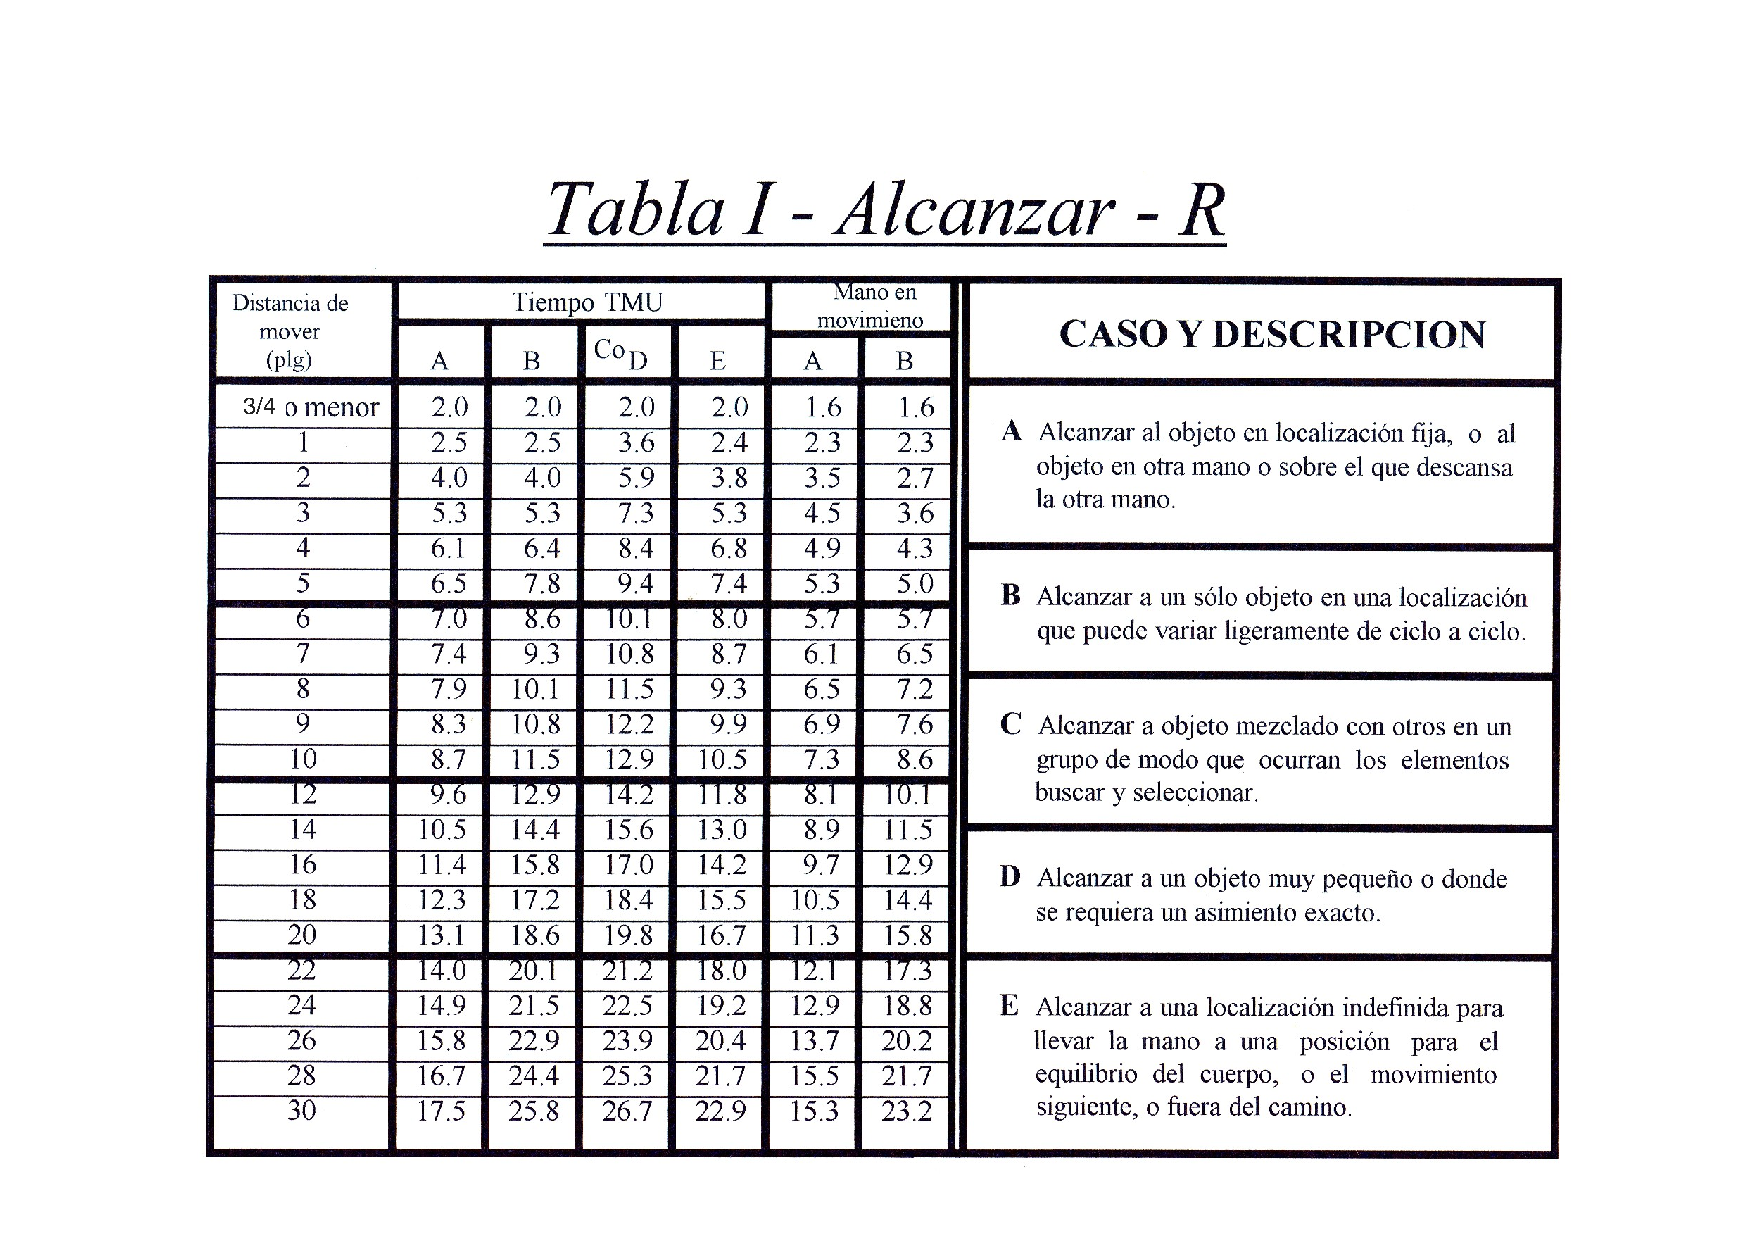
\includegraphics[trim = {20mm 40mm 20mm 25mm},clip,scale=0.25]{9/Img/tablaAlcanzar.pdf}
        \caption{Tabla de tiempos TMU para el movimiento Alcanzar}
        \label{fig:bimanual}
    \end{figure}
    %
    \begin{figure}[H]
        \centering
        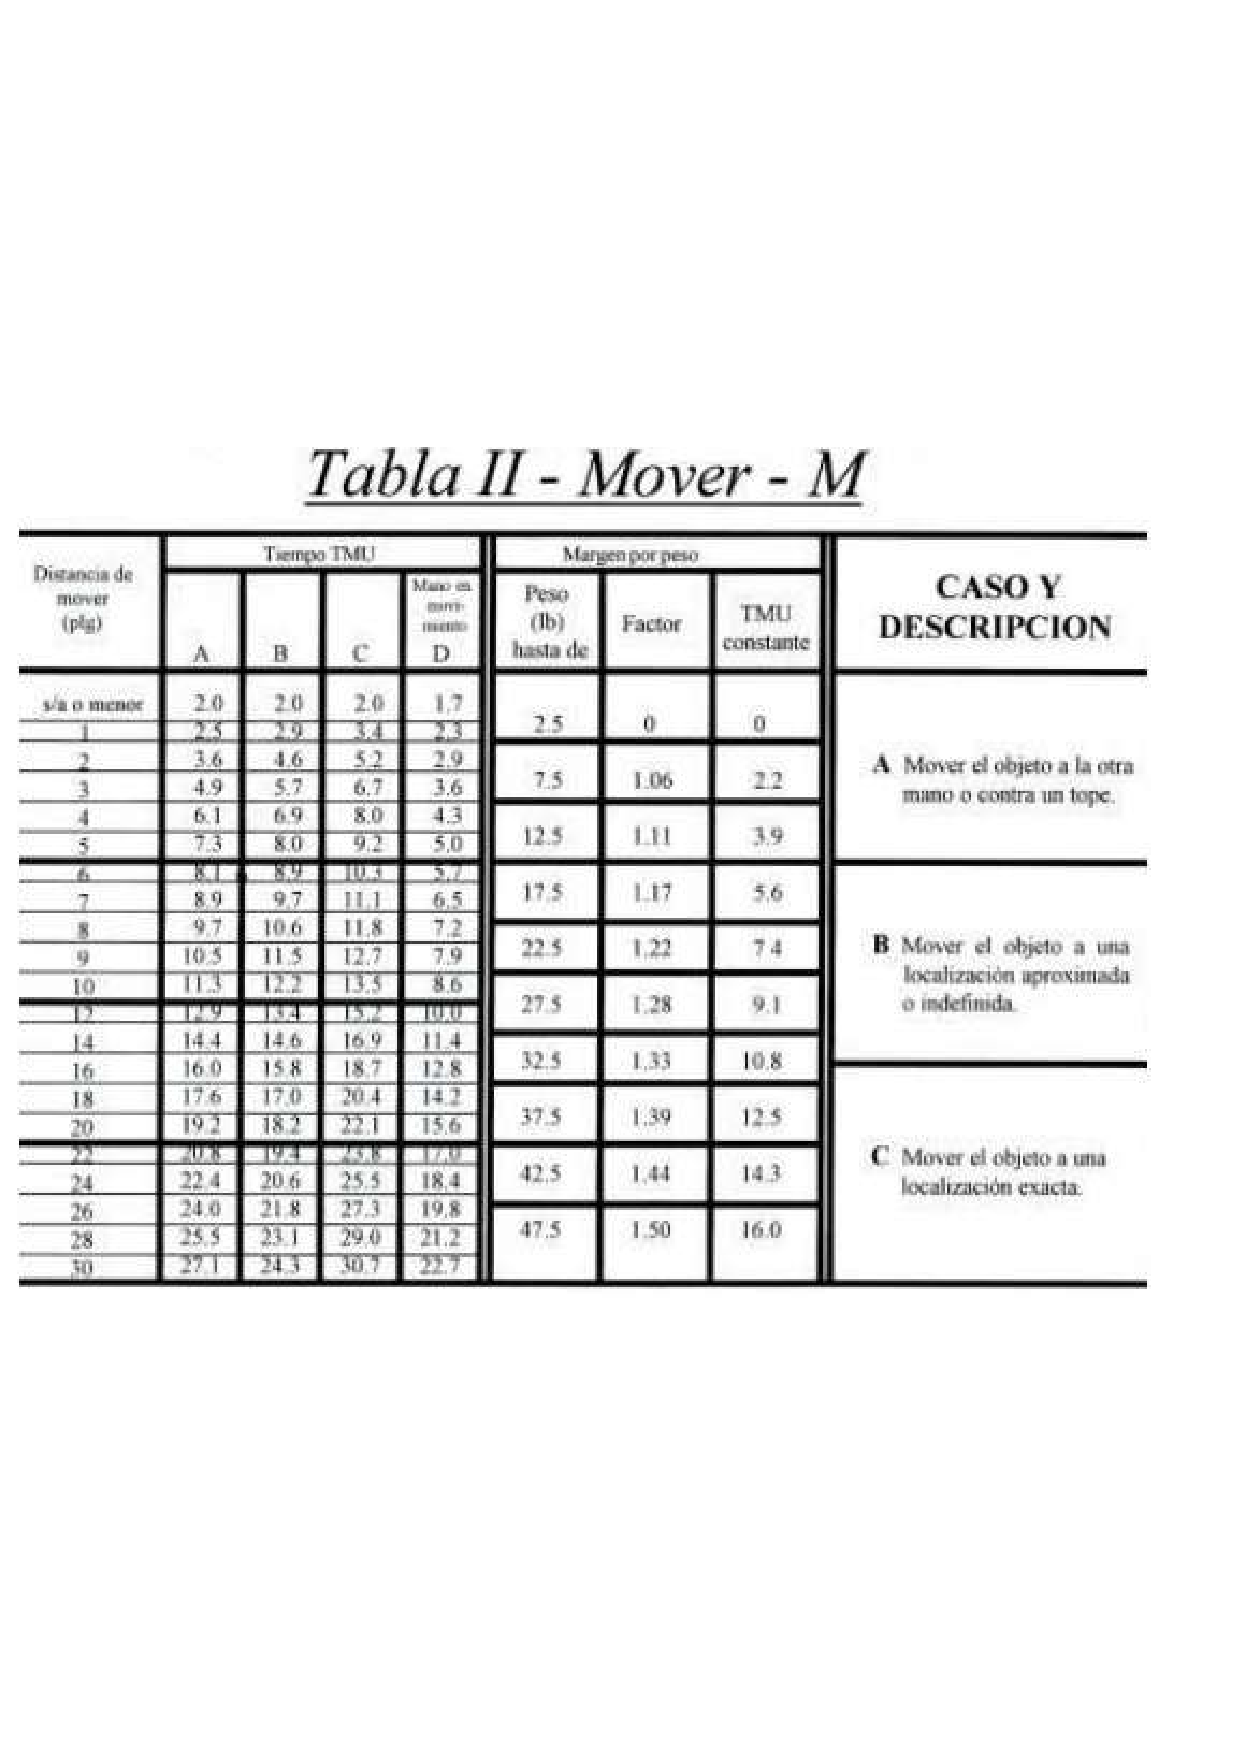
\includegraphics[trim = {20mm 40mm 20mm 25mm},clip,scale=0.25]{9/Img/tablaMover.pdf}
        \caption{Tabla de tiempos TMU para el movimiento Mover}
        \label{fig:bimanual}
    \end{figure}
    %
    \begin{figure}[H]
        \centering
        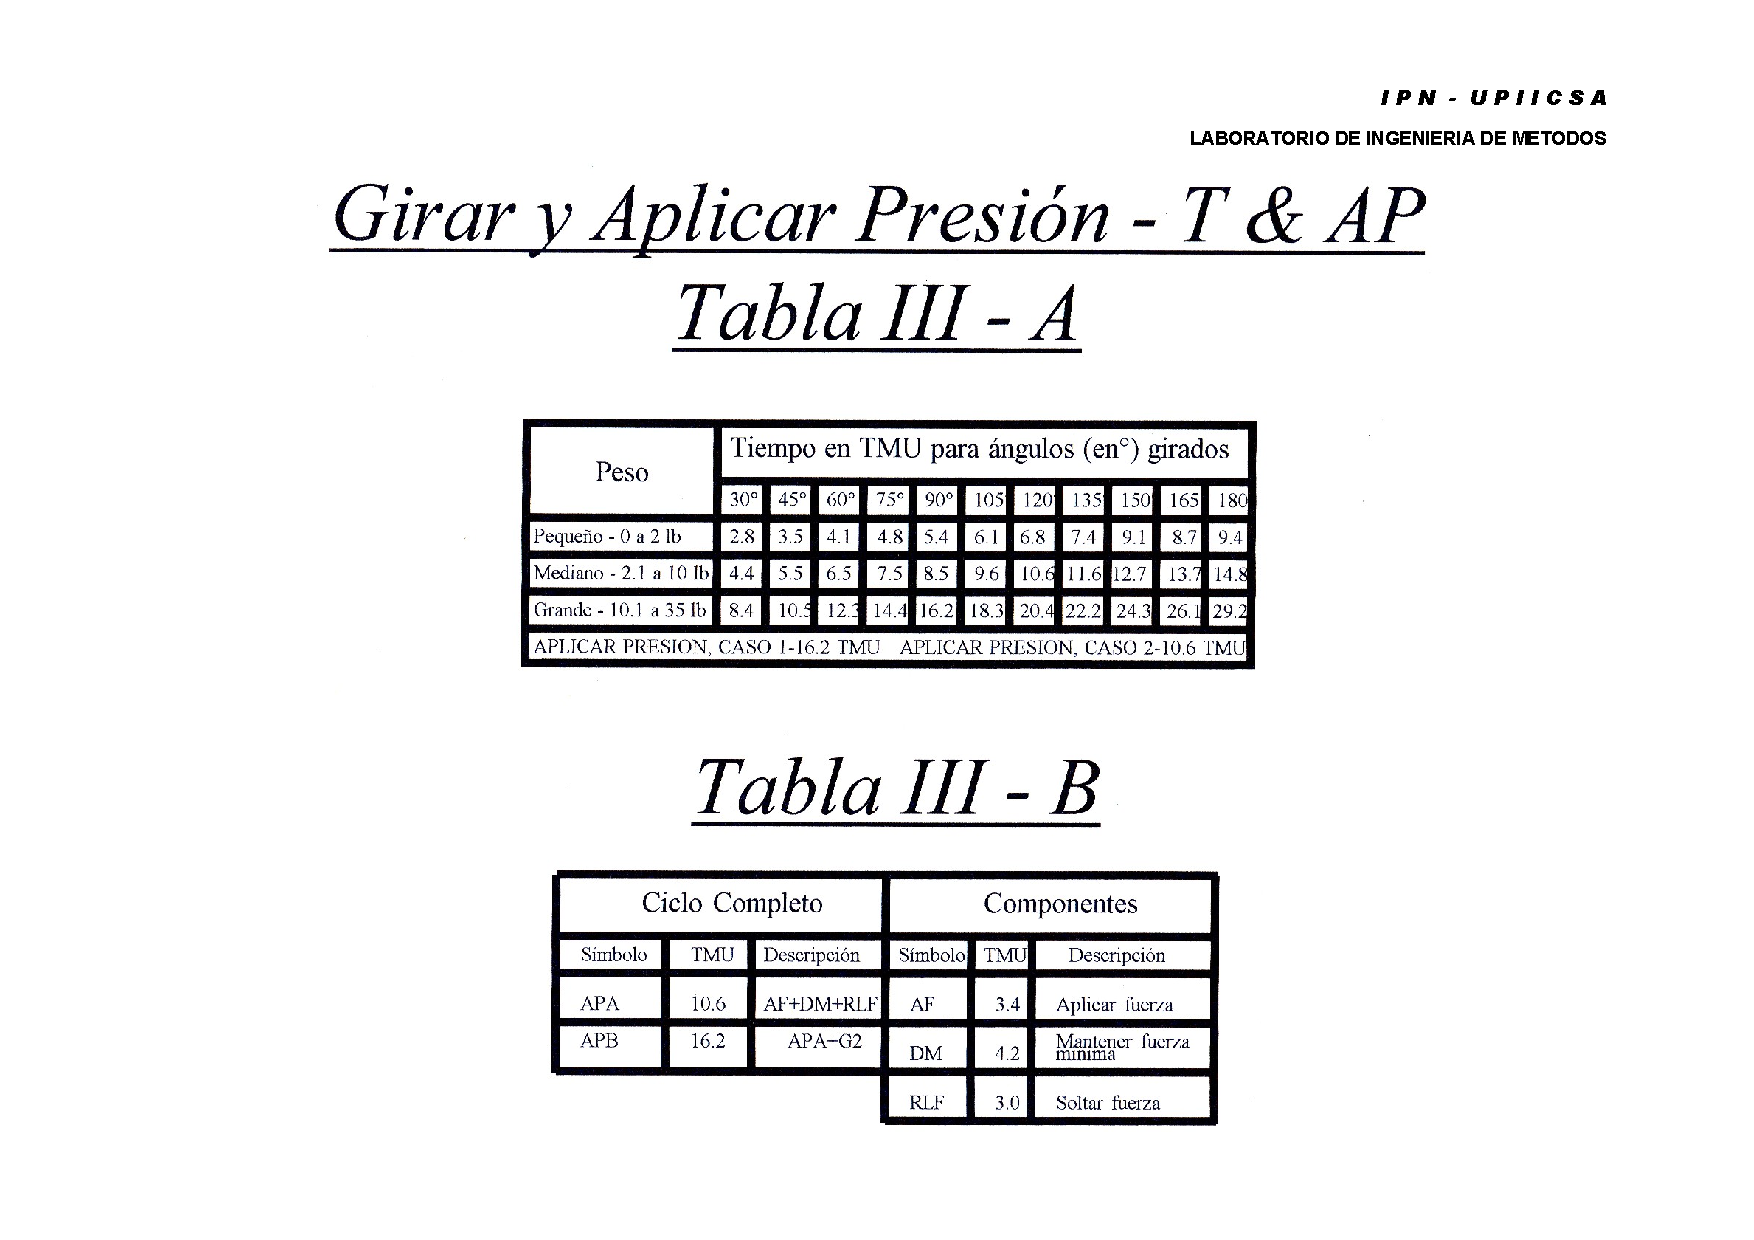
\includegraphics[trim = {20mm 40mm 20mm 25mm},clip,scale=0.25]{9/Img/tablaGirar.pdf}
        \caption{Tabla de tiempos TMU para el movimiento Girar}
        \label{fig:bimanual}
    \end{figure}
    %
    \begin{figure}[H]
        \centering
        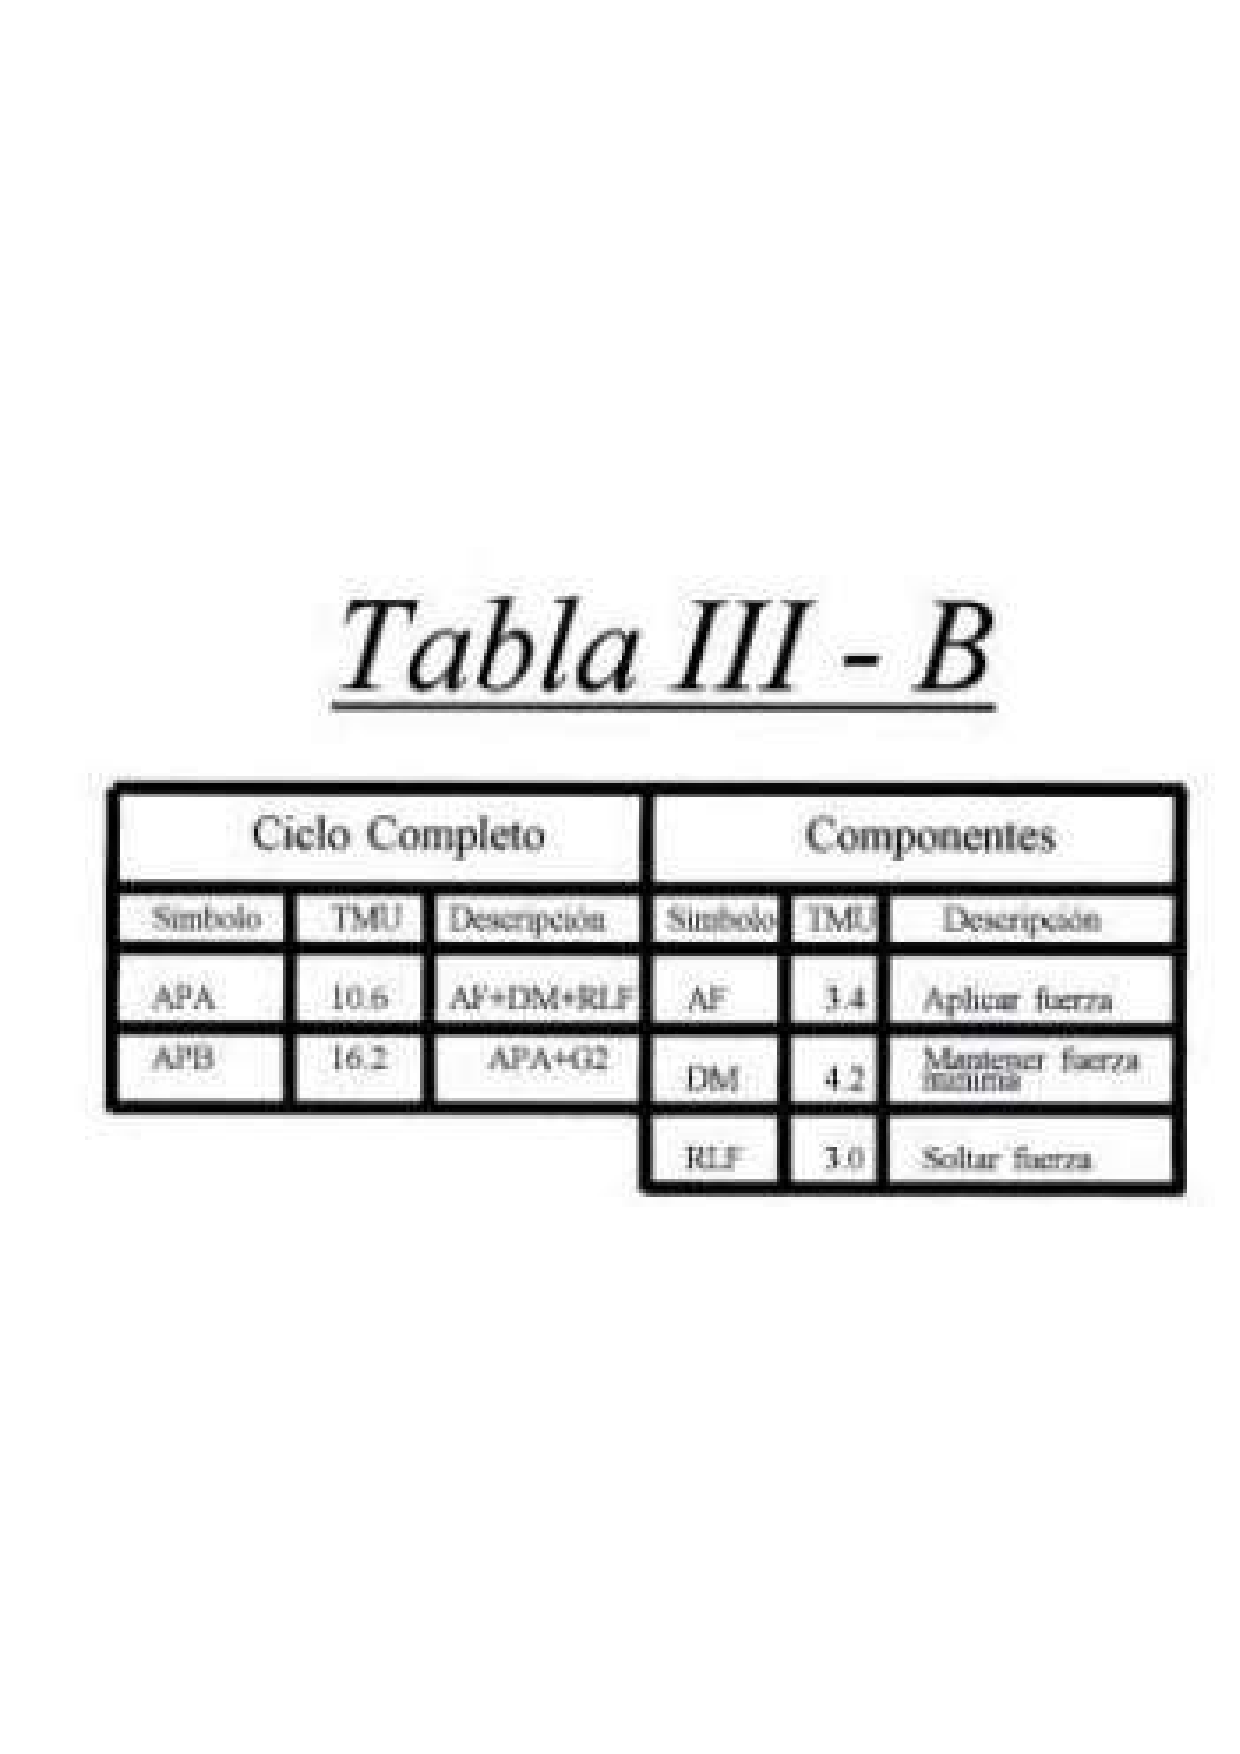
\includegraphics[trim = {20mm 40mm 20mm 25mm},clip,scale=0.25]{9/Img/tablaB.pdf}
        \caption{ Tabla de tiempos TMU para el movimiento Aplicar Presión }
        \label{fig:bimanual}
    \end{figure}
    
    %
    \begin{figure}[H]
        \centering
        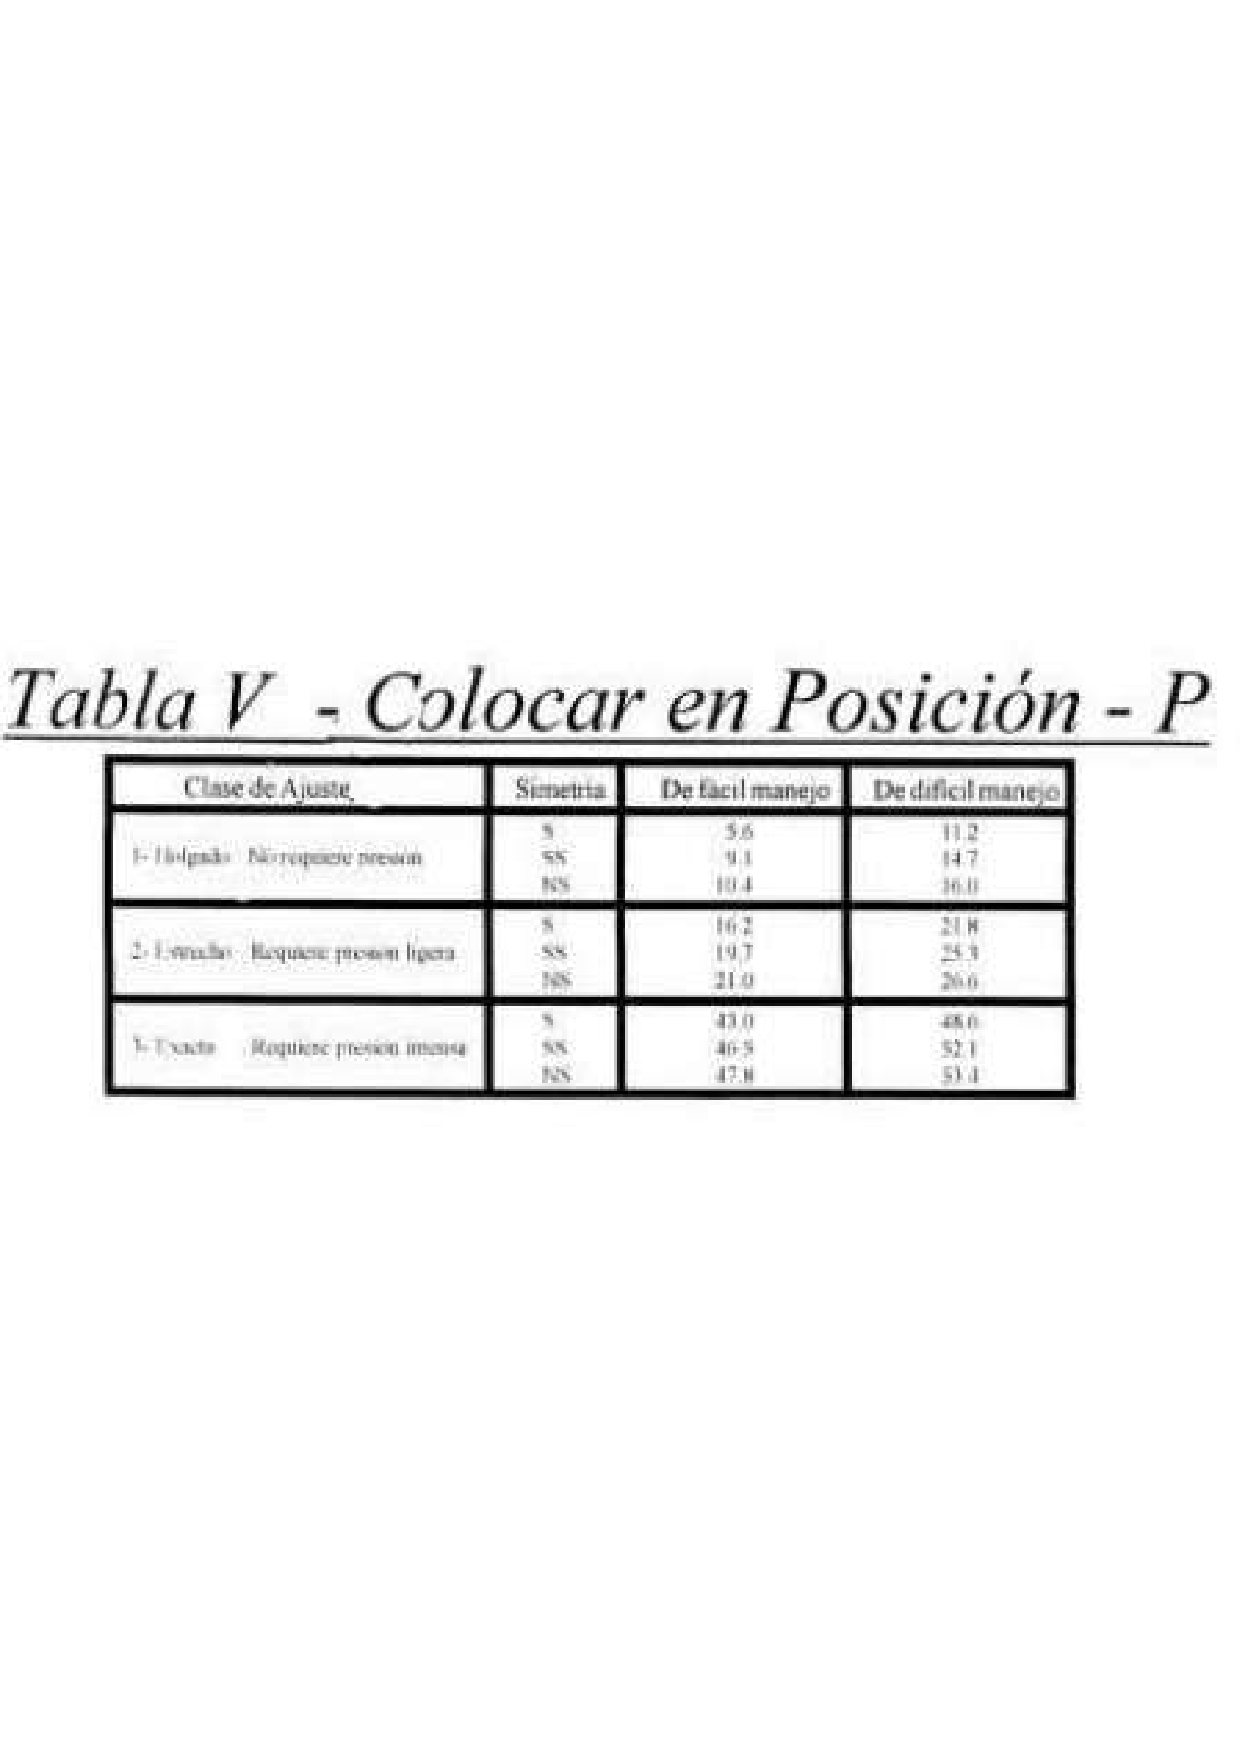
\includegraphics[trim = {20mm 40mm 20mm 25mm},clip,scale=0.25]{9/Img/tablaPosicion.pdf}
        \caption{ Tabla de tiempos TMU para el movimiento Coloca }
        \label{fig:bimanual}
    \end{figure}
    
    %
    \begin{figure}[H]
        \centering
        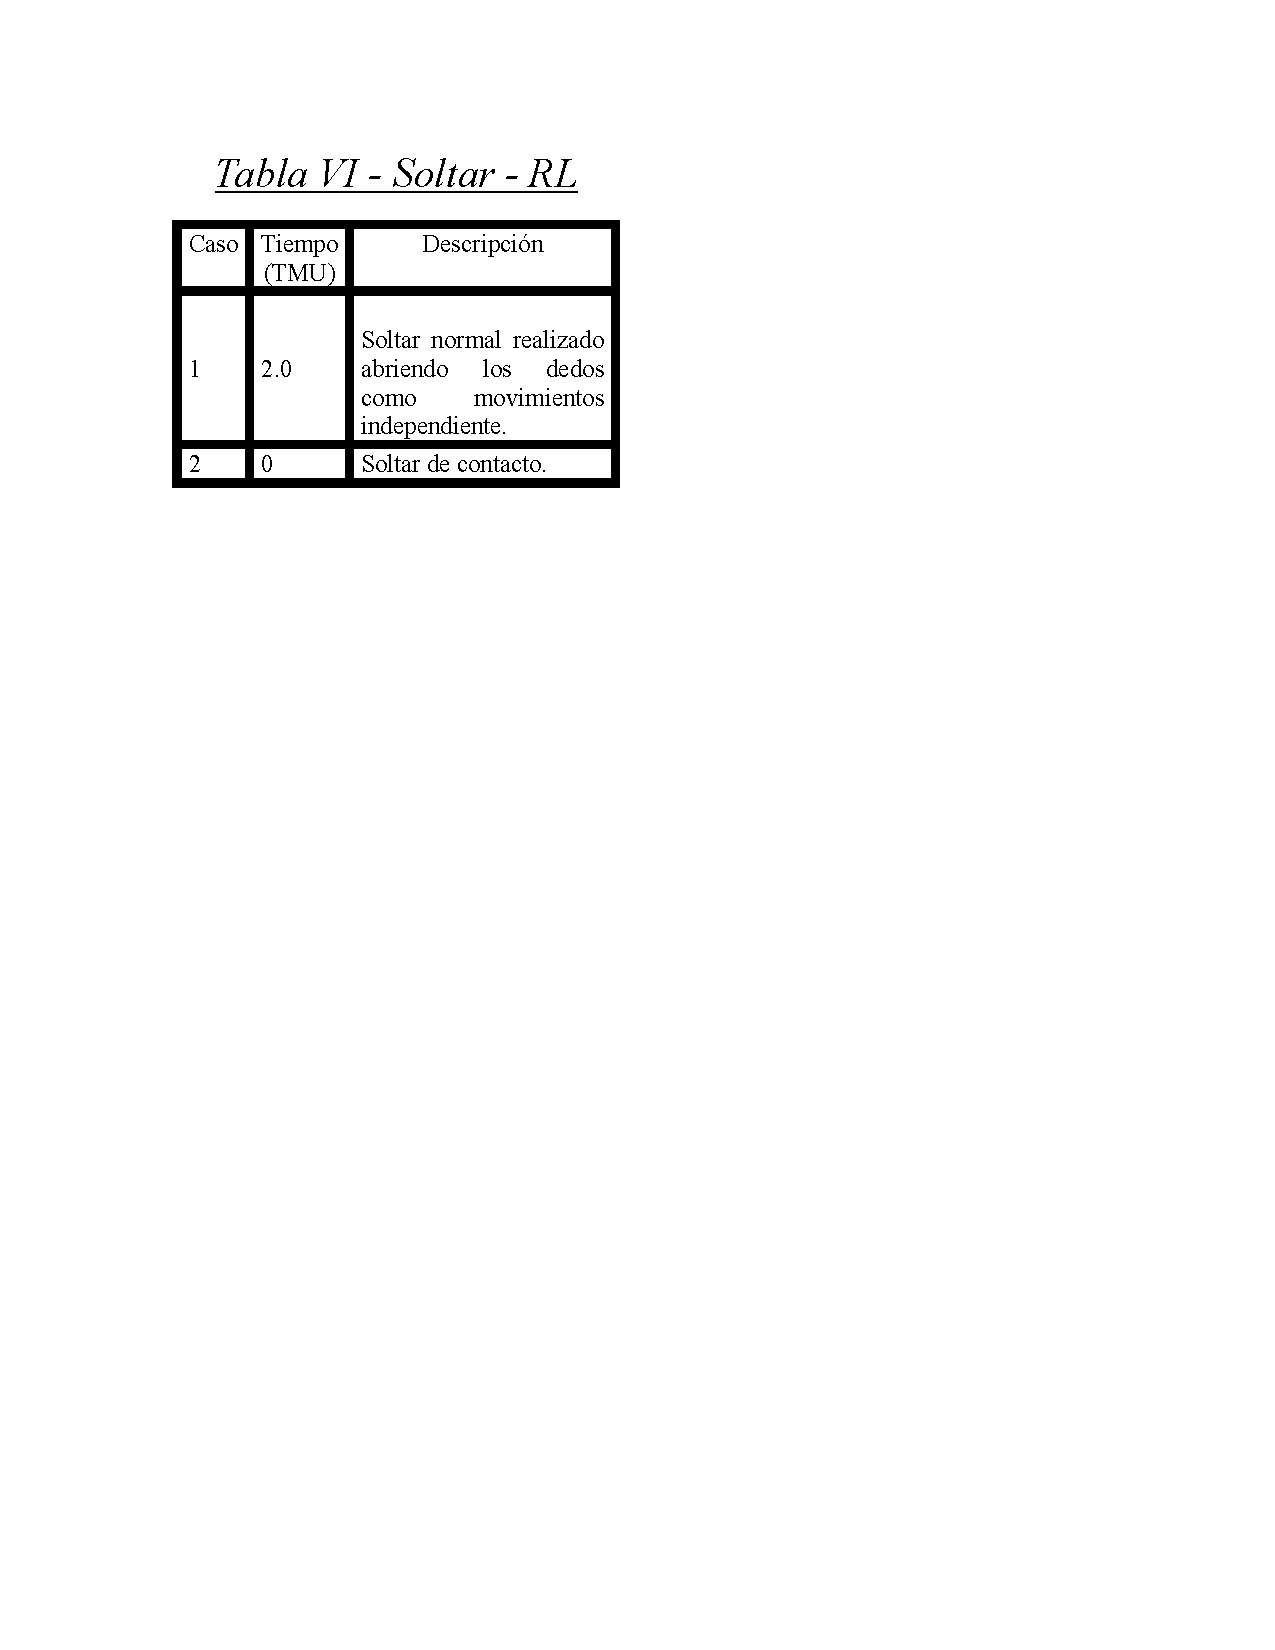
\includegraphics[trim = {20mm 40mm 20mm 25mm},clip,scale=0.25]{9/Img/tablaSoltar.pdf}
        \caption{ Tabla de tiempos TMU para el movimiento Soltar }
        \label{fig:bimanual}
    \end{figure}
    
    
    
    \subsubsection{Desarrollo del muestreo del trabajo}
    % 
    El muestreo del trabajo es una técnica que se basa en seleccionarían muestra representativa con el fin de obtener información relevante para la toma de decisión.\\ 
    Principalmente se debe de llevar varias etapas como: Definición del objetivo la cual permitirá determinar cual es la población objetiva.
    Selección de la población: Identificar la población objetivo en la que se va a realizar el muestreo.
    Determinación del tamaño de la muestra: Es la que depende del tamaño de la población, el margen del error.
    %
    \begin{figure}[H]
        \centering
        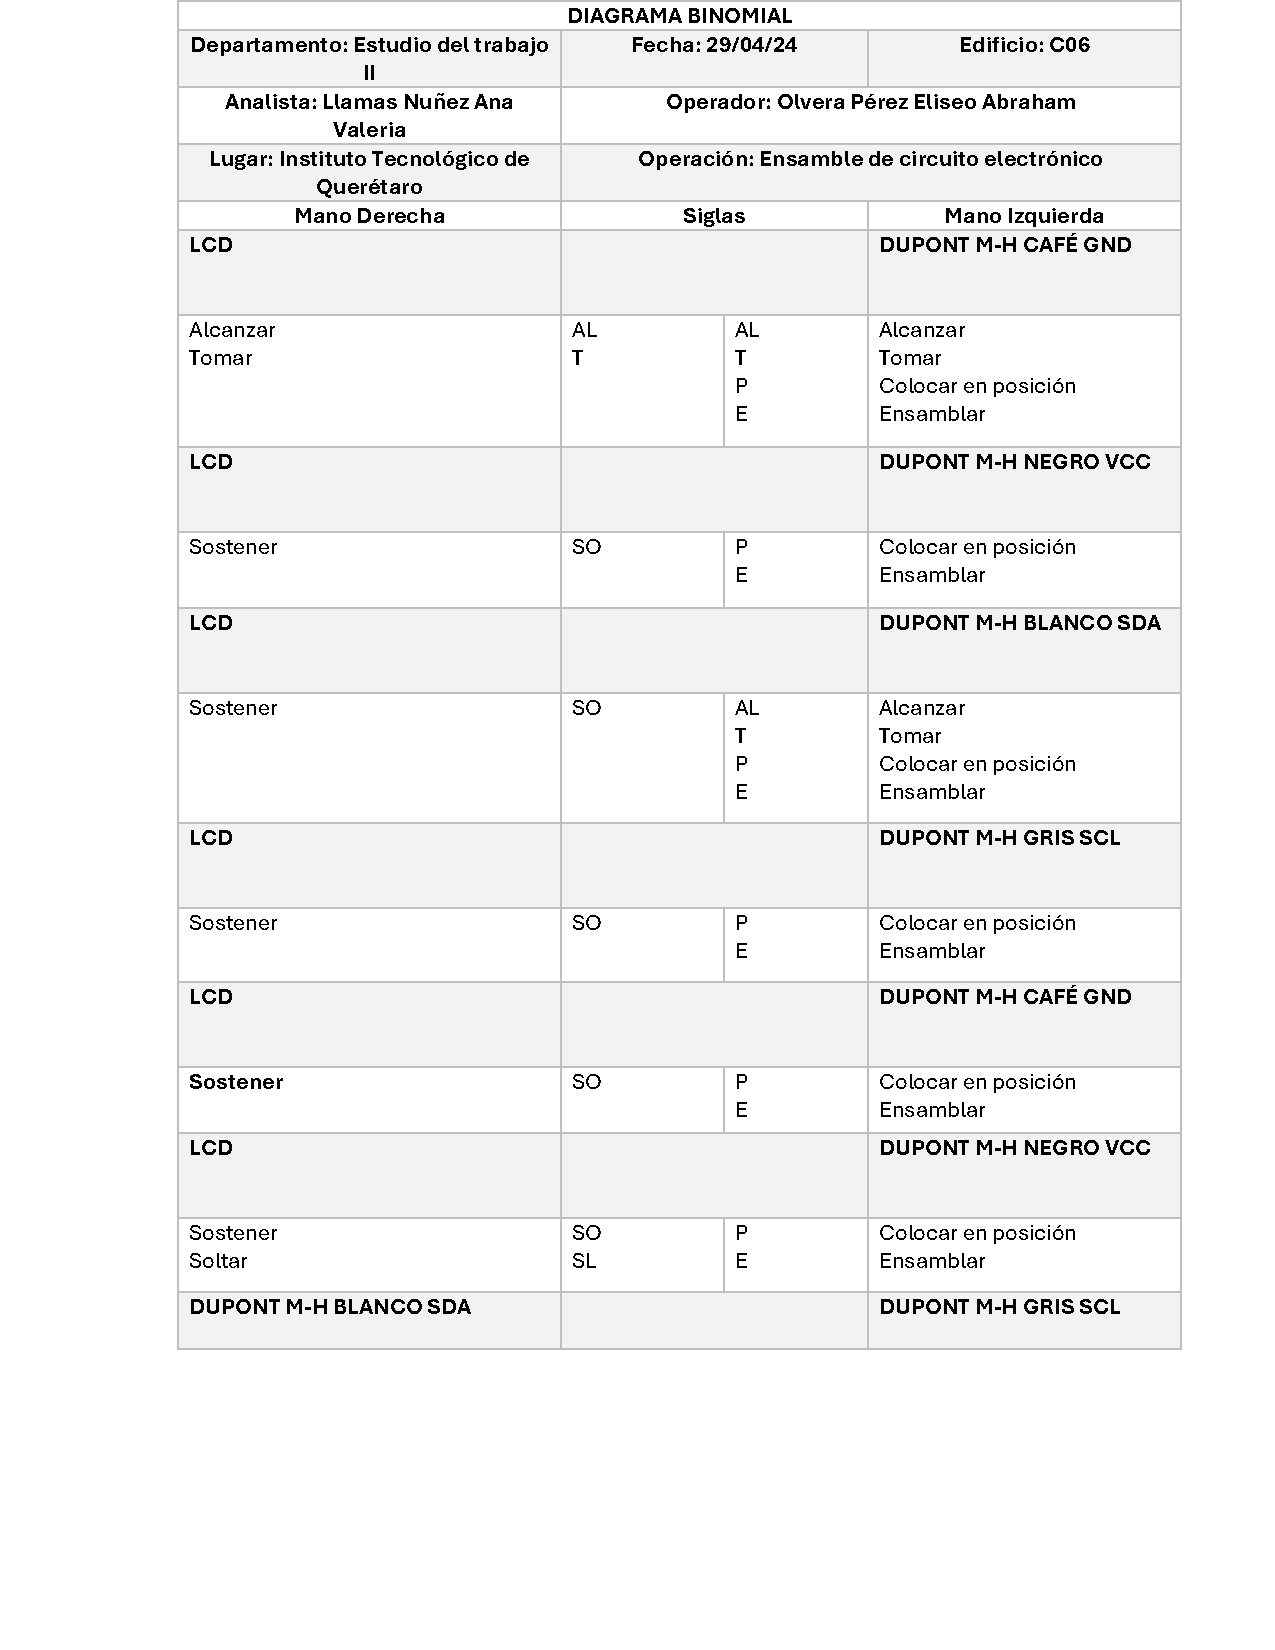
\includegraphics[trim = {20mm 82mm 20mm 25mm},clip,scale=0.45]{9/Img/tablaBimanual.pdf}
        \caption{TABLA BIMANUAL }
        \label{fig:bimanual}
    \end{figure}
    %
    \begin{figure}[H]
        \centering
        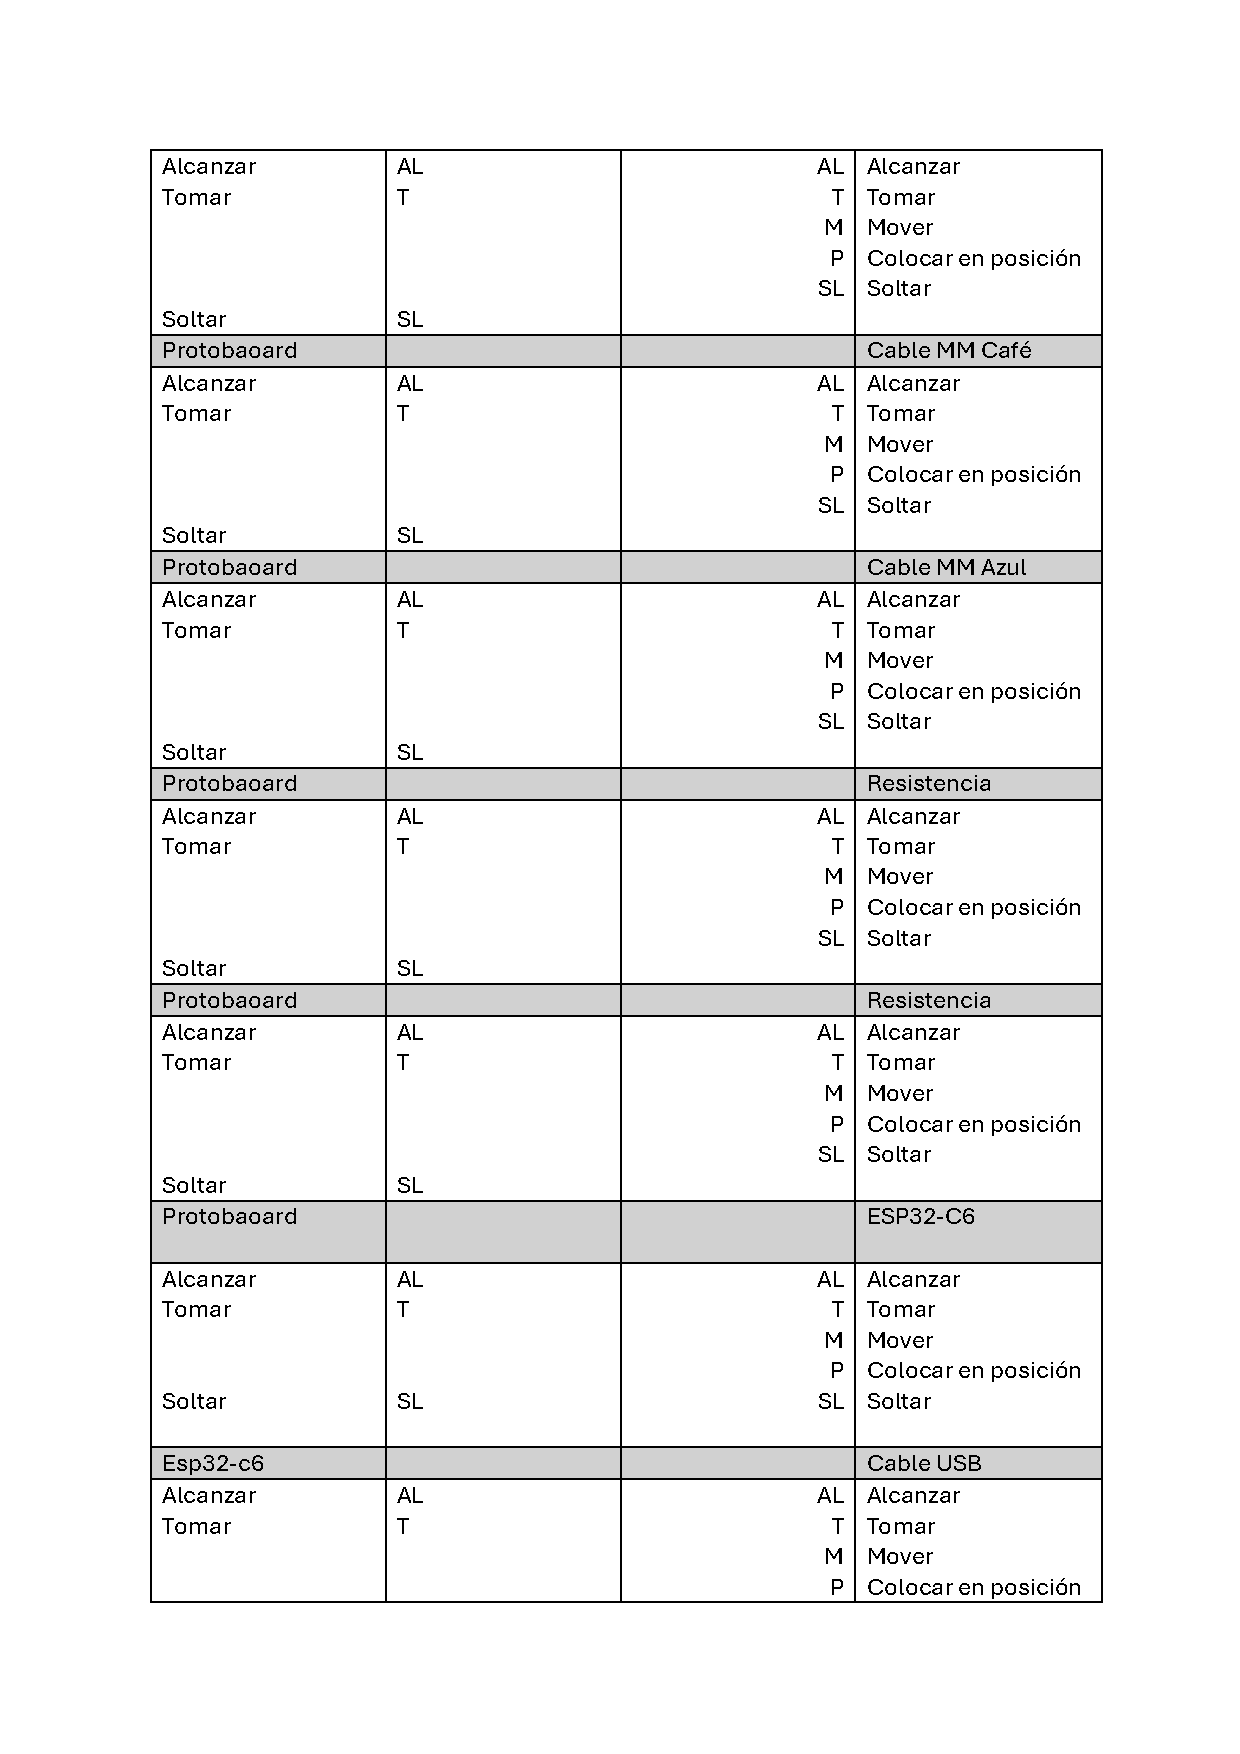
\includegraphics[trim = {20mm 82mm 20mm 25mm},clip,scale=0.45]{9/Img/tablaBimanualDos.pdf}
        \caption{TABLA BIMANUAL }
        \label{fig:bimanual}
    \end{figure}
    %
    \begin{figure}[H]
        \centering
        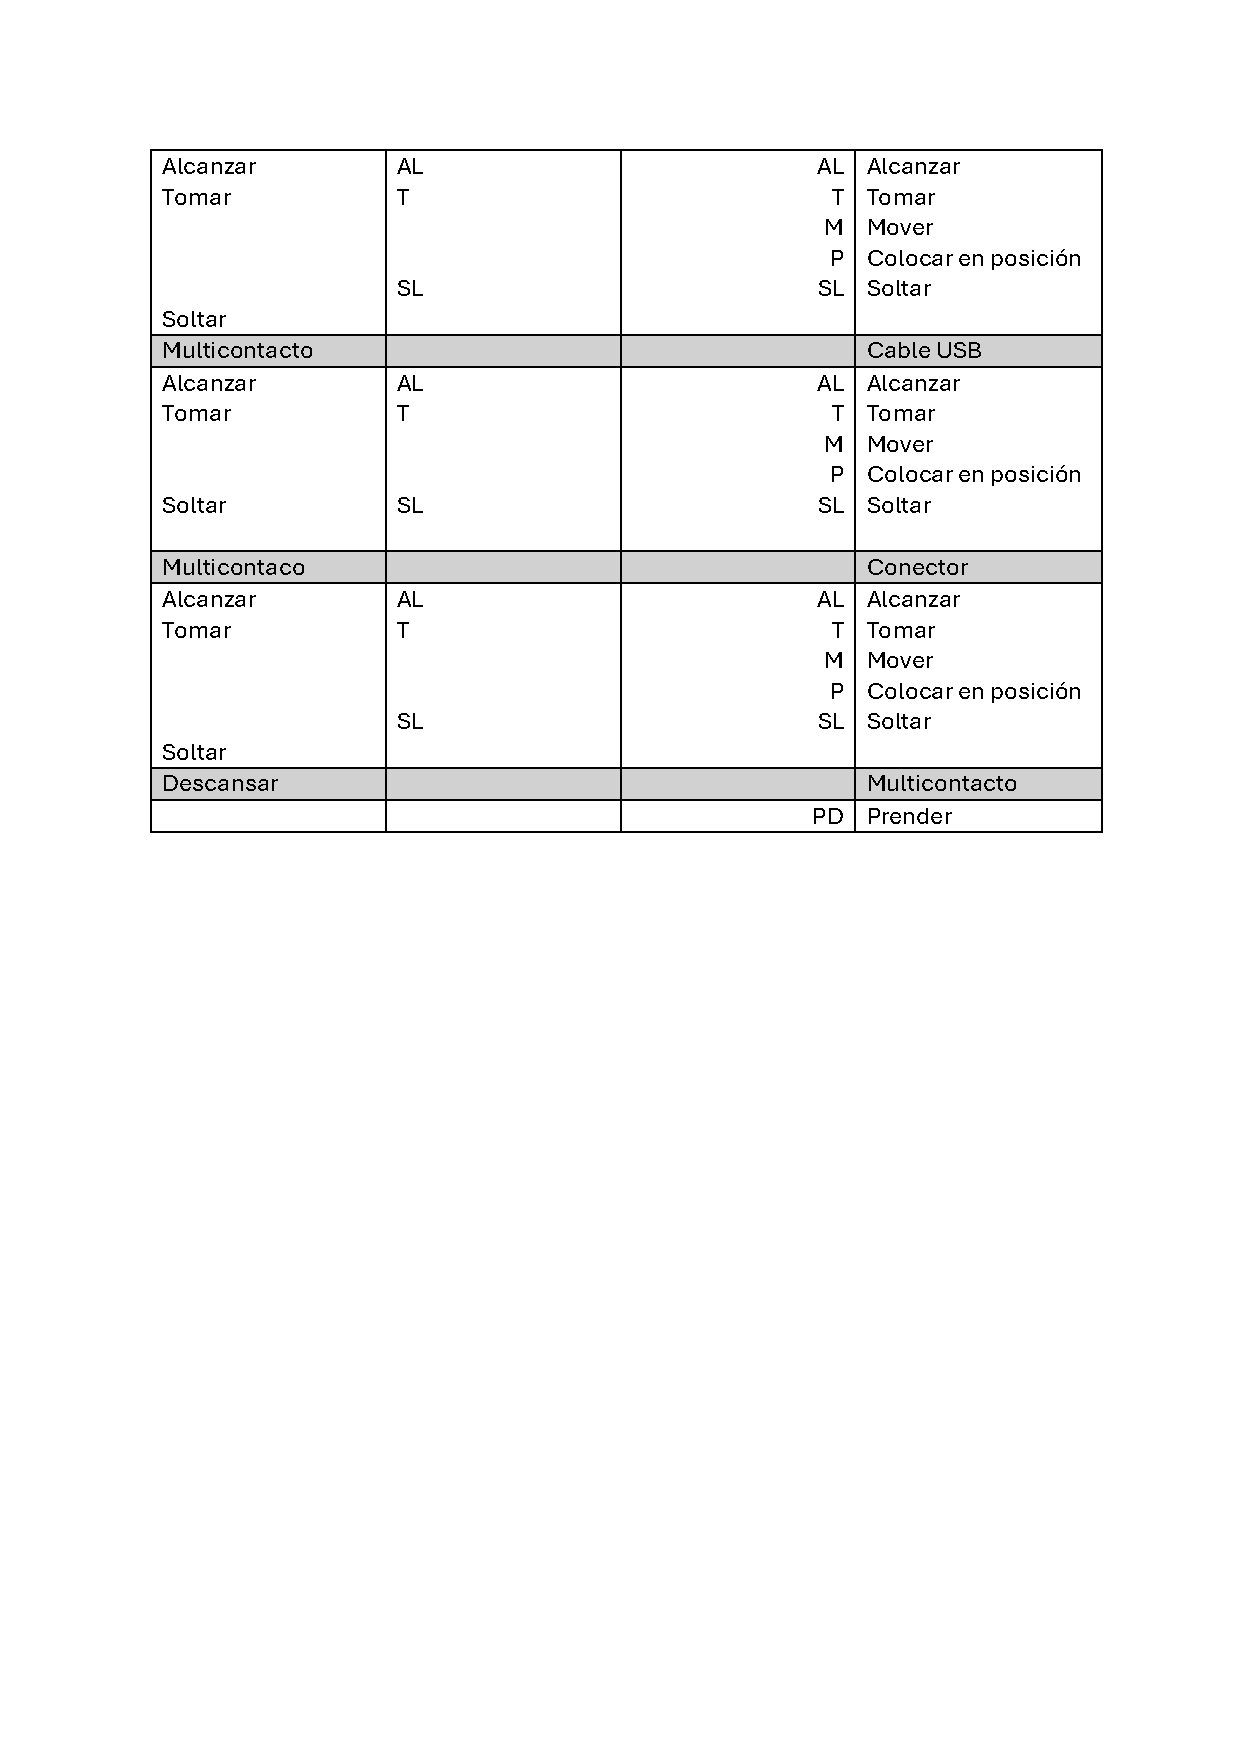
\includegraphics[trim = {20mm 82mm 20mm 25mm},clip,scale=0.45]{9/Img/tablaBimanualTres.pdf}
        \caption{TABLA BIMANUAL }
        \label{fig:bimanual}
    \end{figure}
    %
    
     
    % 
    \subsubsection{Corrección por balanceo de procesos}
    % 
    La corrección por balanceo de procesos se refiere a la técnica utilizada en sistemas informáticos para una distribución equitativamente entre los diferentes procesadores de un sistema computacional. 
    Este balanceo de procesos nos ayudara en el proyecto para la corrección  del proceso del ensamble para optimizar el rendimiento del sistema con la finalidad de cada linea de producción tenga continuidad y cuente con un tiempo proceso uniforme para evitar cuellos de botella o algún retrasado en la linea de producción.\\
    Para lograr un balance adecuado es importante el analizar el tiempo , así como las habilidades que se deben considerar como la disponibilidad y el buen manejo de herramientas y materiales.
    % 
    \subsubsection{Datos estándar continuos y discretos}
    % 
    Los datos estándar se refieren a un conjunto de información que ha sido establecida como un modelo o referencia para comparar o medir otras variables es el tiempo estándar requerido para la ejecución de un proceso. Estos datos suelen ser utilizados como punto de referencia para evaluar el desempeño de un sistema o una organización.\\
    Los datos estándar continuos son aquellos que pueden tomar cualquier valor dentro de un rango específico, son necesarios los estudios de tiempo y movimientos, análisis.\\
    Los datos estándar discretos son aquellos que solo pueden tomar valores específicos y separados entre sí, estos datos son fundamentales en la materia de estudio del trabajo.\\
    % 
    \subsection{Diseño de la forma más económica de realizar el trabajo}
    %
     Este diseño es fundamental para maximizar la eficiencia y reducir los costos de construcción de circuitos electrónicos. Para lograrlo, es necesario examinar detalladamente cada etapa del proceso de ensamblaje en busca de oportunidades de optimización en términos de costos de materiales y recursos utilizados. Esto incluye analizar el flujo de trabajo, el tiempo requerido para cada tarea, los recursos humanos y tecnológicos involucrados, y los materiales utilizados. Al mejorar estos aspectos, se pueden reducir los costos totales y aumentar la rentabilidad del proceso de producción sin comprometer la calidad y funcionalidad del producto final.
    % 
    \subsection{Normalización de los métodos, materiales, herramientas e instalaciones}
    %
    Se está estandarizando los elementos necesarios para llevar a cabo un nuevo método de ensamblaje.\\ La metodología establecida para obtener los valores de cada ciclo implica presentar los materiales a utilizar en el proceso de ensamblaje, en un formato fácil de entender con una imagen de referencia. Se entregará un manual que incluirá un modelo 3D de la pieza, su costo unitario en el mercado y la cantidad aproximada de piezas requeridas. Se hace hincapié en la utilización del protoboard, una placa con agujeros y conexiones eléctricas en su interior para la creación de circuitos eléctricos. Se menciona la soldadura para suministrar directamente energía al procesador. También se explica la resistencia como una pieza de plástico con alambre usada en los circuitos eléctricos para regular el flujo de corriente.
    % 
    \begin{table}[H]
        \centering
        \caption{MATERIALES}
        \begin{tabular}{|c |c |}
        \hline
        \multicolumn{2}{c}{MODELOS}\\
        \hline
             Esp32& \ 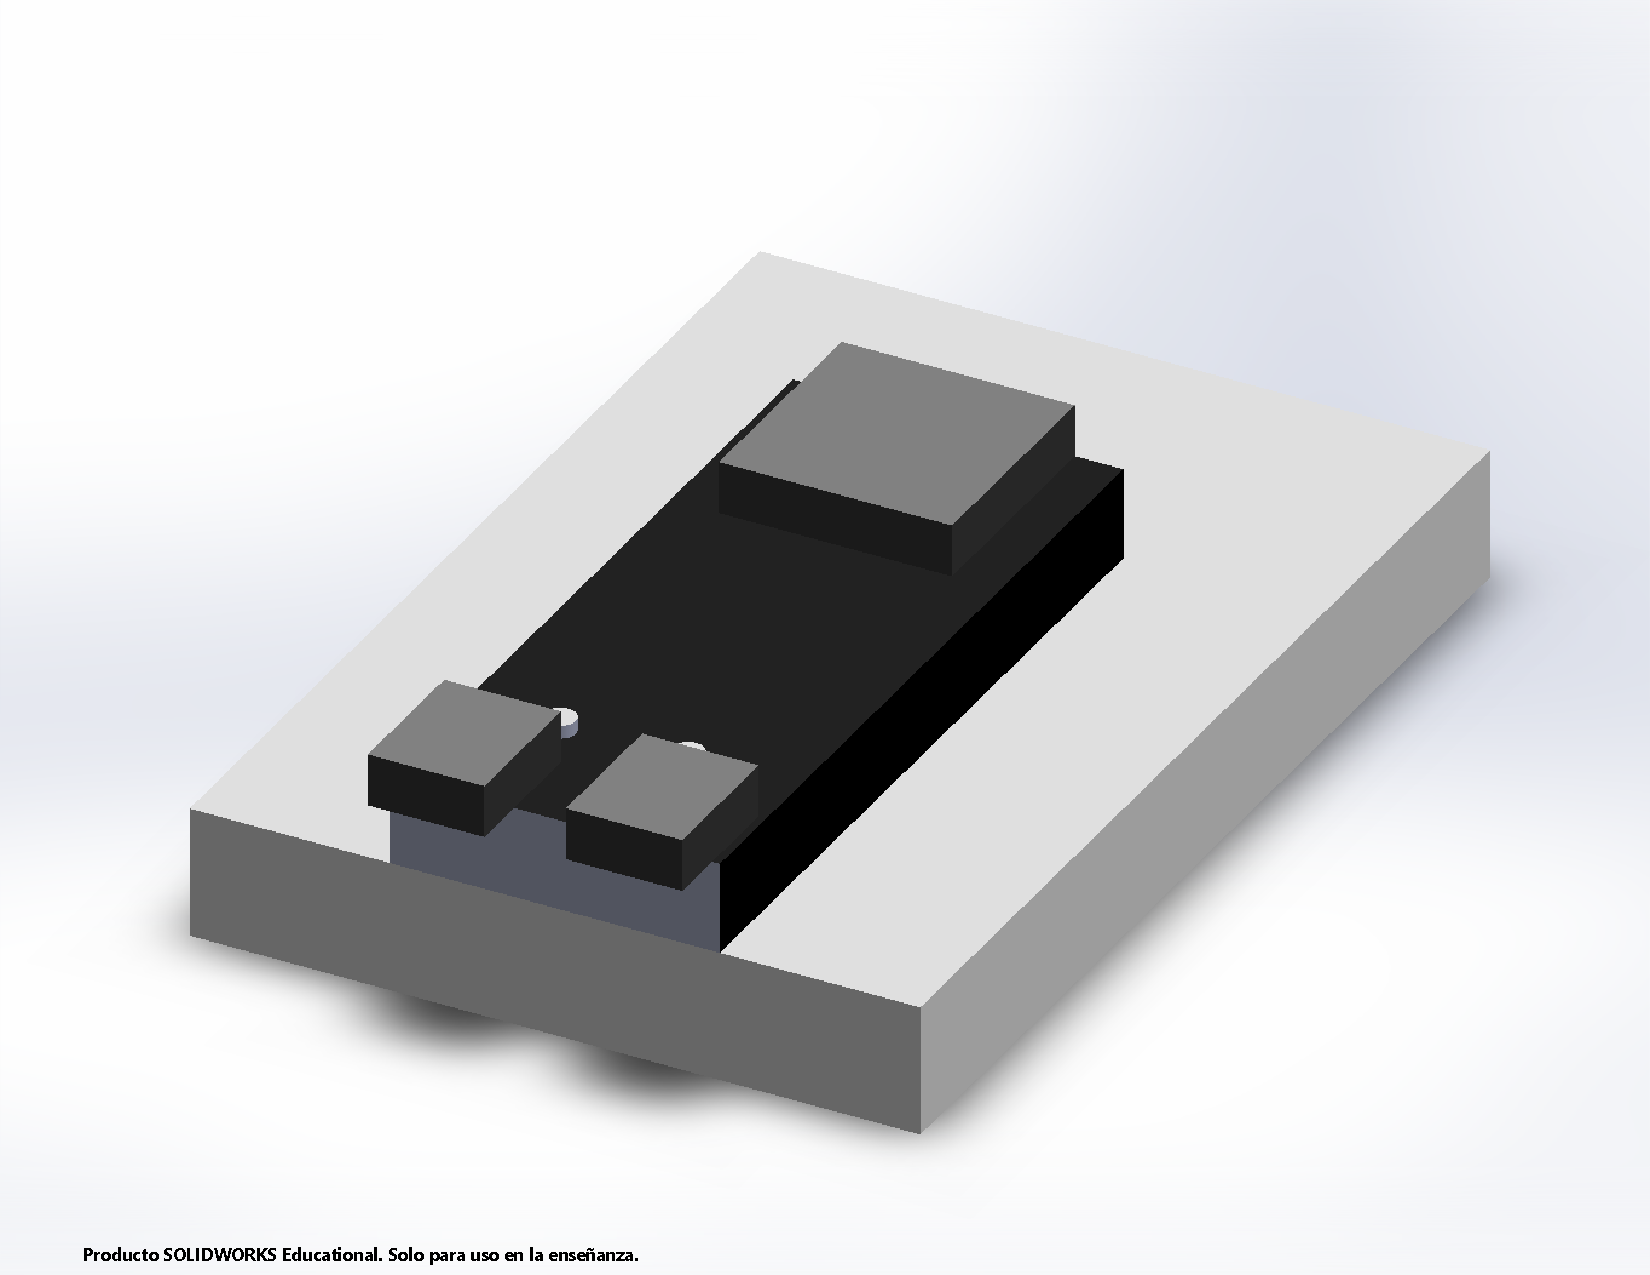
\includegraphics[scale=0.1]{9/Img/piezaEsp32.pdf}\\
        \hline
             LCD& 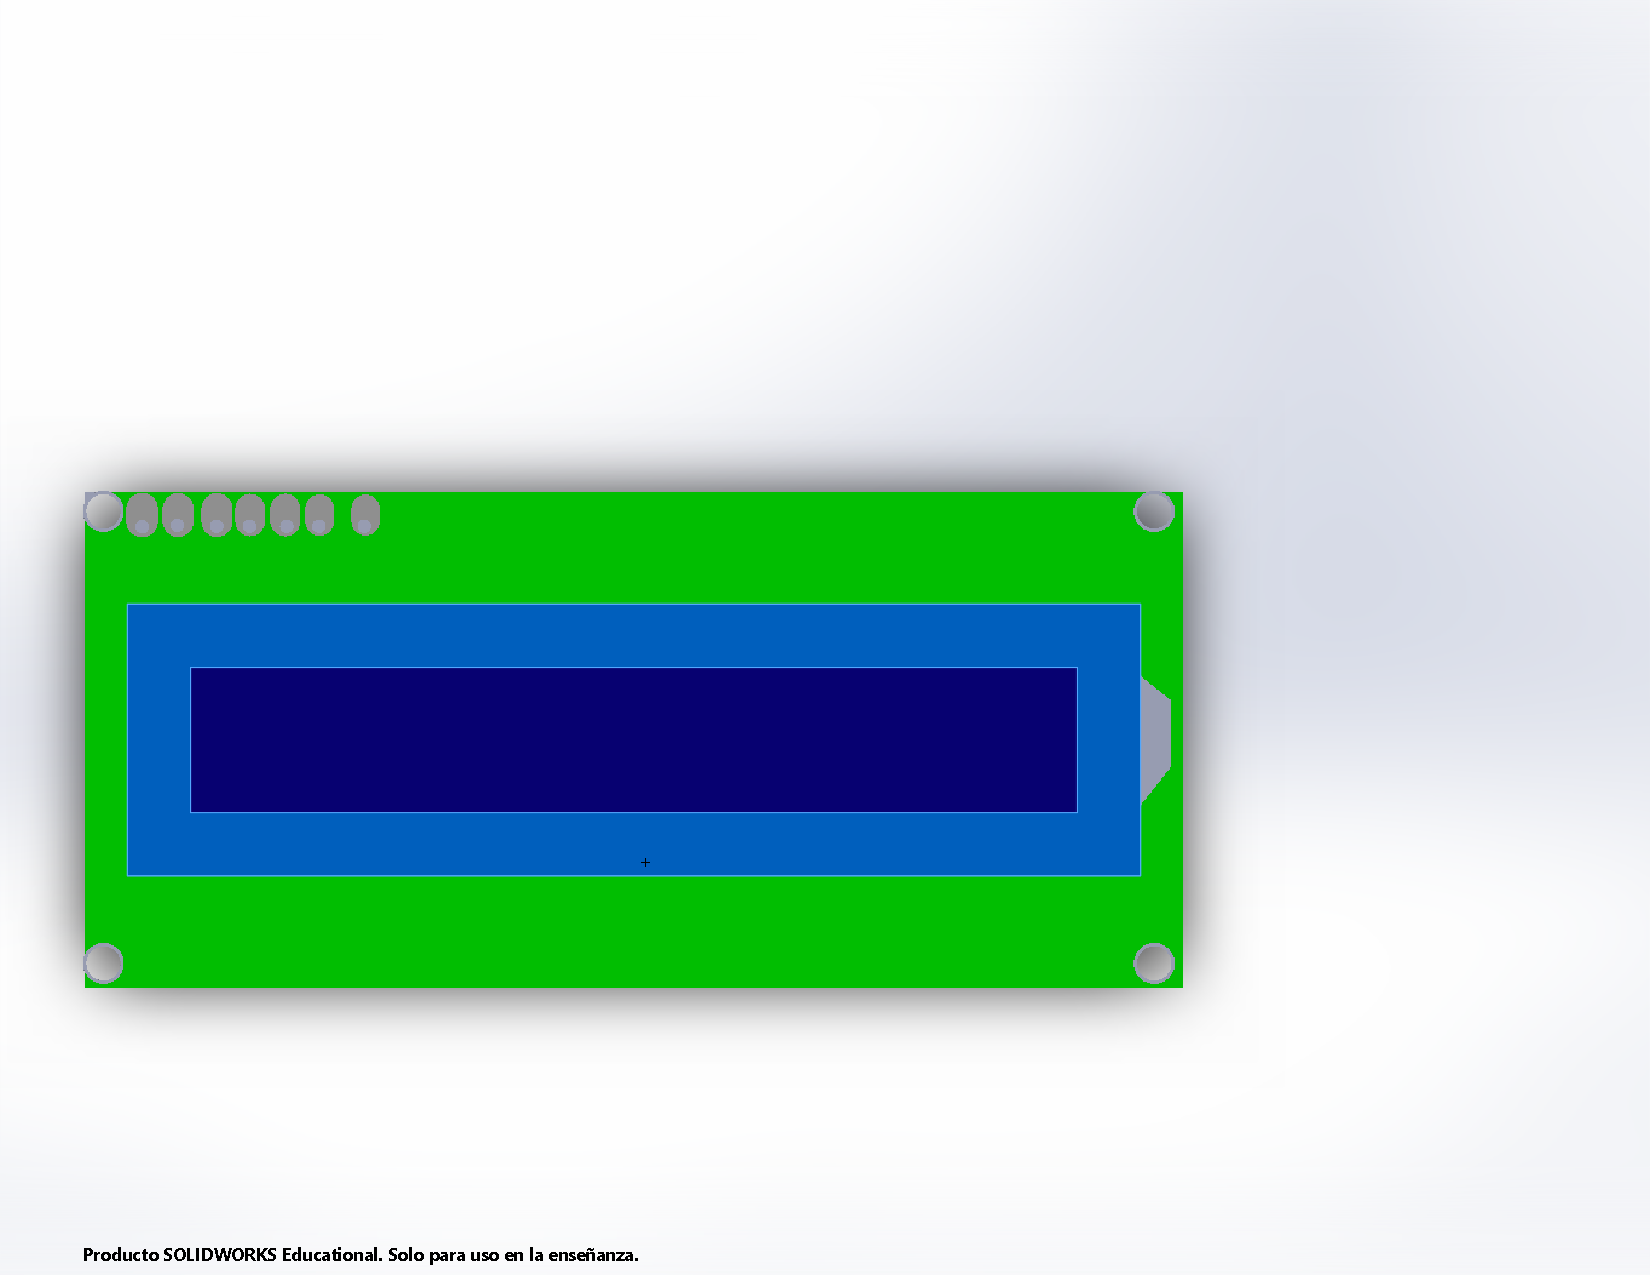
\includegraphics[scale=0.1]{9/Img/piezaLcd.pdf}   \\
        \hline
             Potenciómetro & 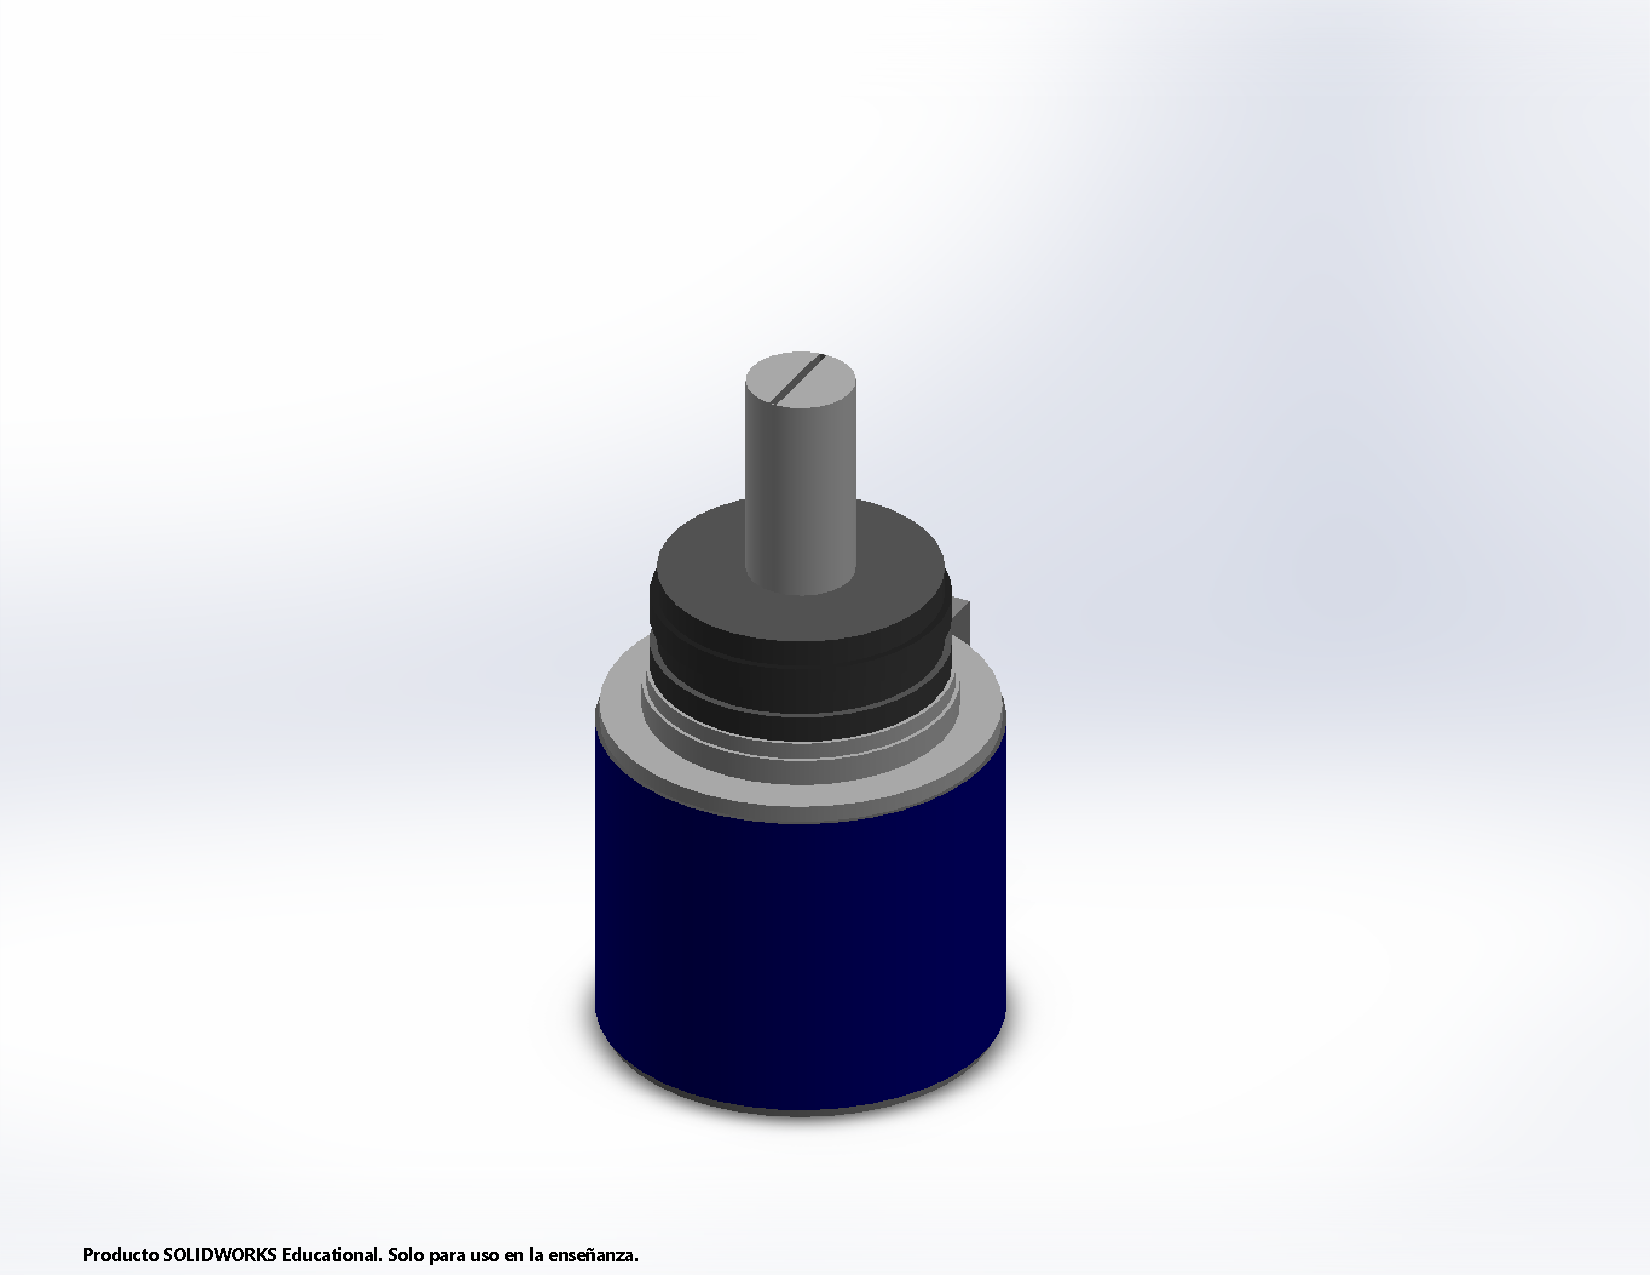
\includegraphics[scale=0.1]{9/Img/piezaPotenciometro.pdf}   \\
        \hline
             Resistencia& \includegraphics[scale=0.1]{9/Img/piezaesistencia.pdf}  \\
        \hline 
             Mm& \includegraphics[scale=0.1]{9/Img/piezaCableMM.PDF}  \\
        \hline
        \end{tabular}
        \label{tab:inventario}
    \end{table}
    %
    \subsection{Determinación del tiempo estándar para que una persona competente realice el trabajo con marcha normal}
    %
    Es necesario realizar un tiempo ciclo y un tiempo estándar, para lograr realizarlas es necesario tablas y formulas las cuales serán vistas en este proyecto.
    Se determina sumando el tiempo asignado a todos los elementos comprendidos en el estudio de tiempos
    %
    
    
    \section{Resultados y discusión}
    
    
    \subsection{Desarrollo de la guía de plan de Emergencia}
    %
    Esta guía es un documento detallado que proporciona instrucciones claras sobre cómo actuar en caso de emergencias como incendios, inundaciones, terremotos, entre otros eventos que puedan poner en peligro la seguridad y el bienestar de los alumnos del Instituto Tecnológico De Querétaro
    %
    
    \begin{figure}[H]
        \centering
        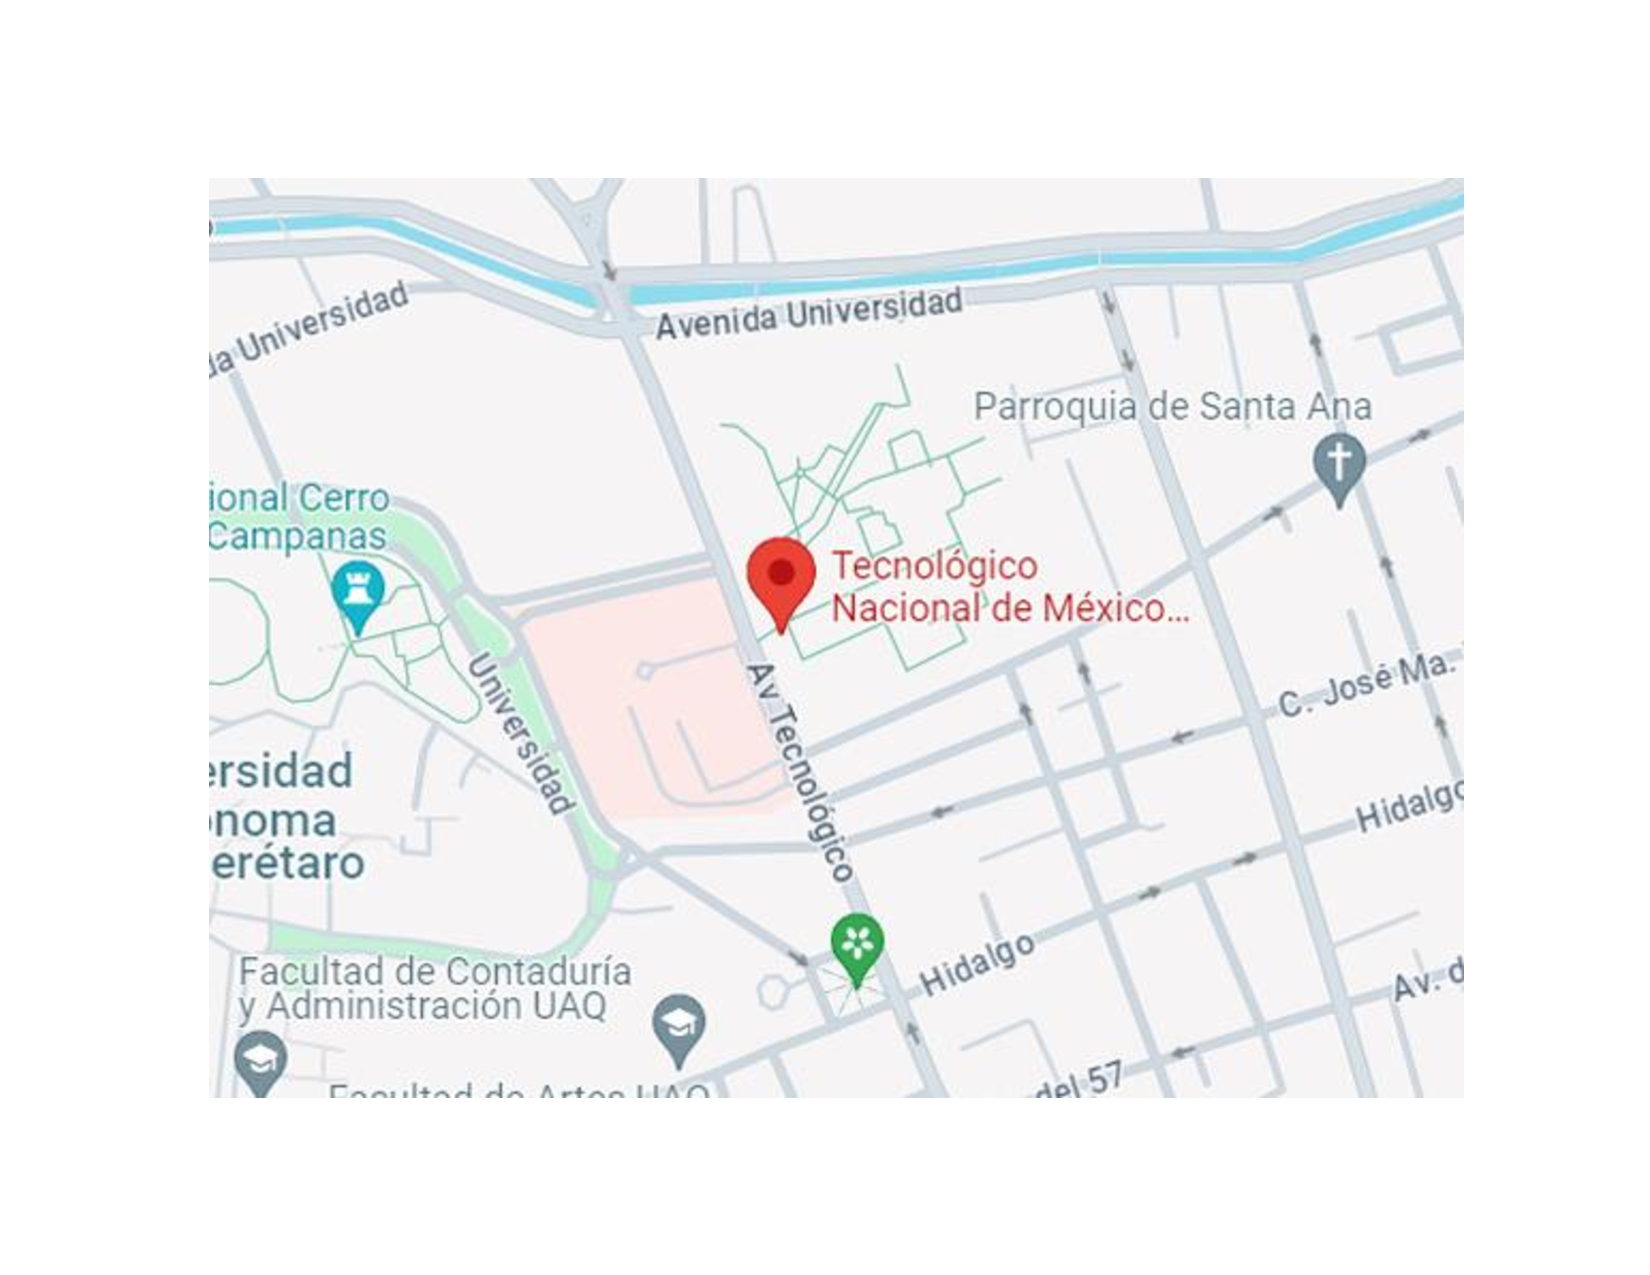
\includegraphics[scale=0.1]{9/Img/mapaItq.pdf}
        \caption{Tecnológico Nacional de México, Instituto Tecnológico de Querétaro, Av Tecnológico S/N, Centro Histórico, Centro, 76000, Querétaro, Qro., 4422274400 Ext. 4423}
        \label{fig:mapa-itq}
    \end{figure}
     
    %
    %
    \subsubsection{Identificación del riesgo}
    %
    Es importante tener en cuenta tanto los riesgos internos, como los externos, y evaluar su probabilidad de ocurrencia y su impacto en el proyecto, ya que es un proceso continuo que requiere de una buena Planificación y Coordinación.\\
    Por lo tanto, es importante revisar regularmente y actualizar el análisis de riesgos para garantizar que se estén abordando de manera efectiva.
    %
    \begin{figure}[H]
        \centering
        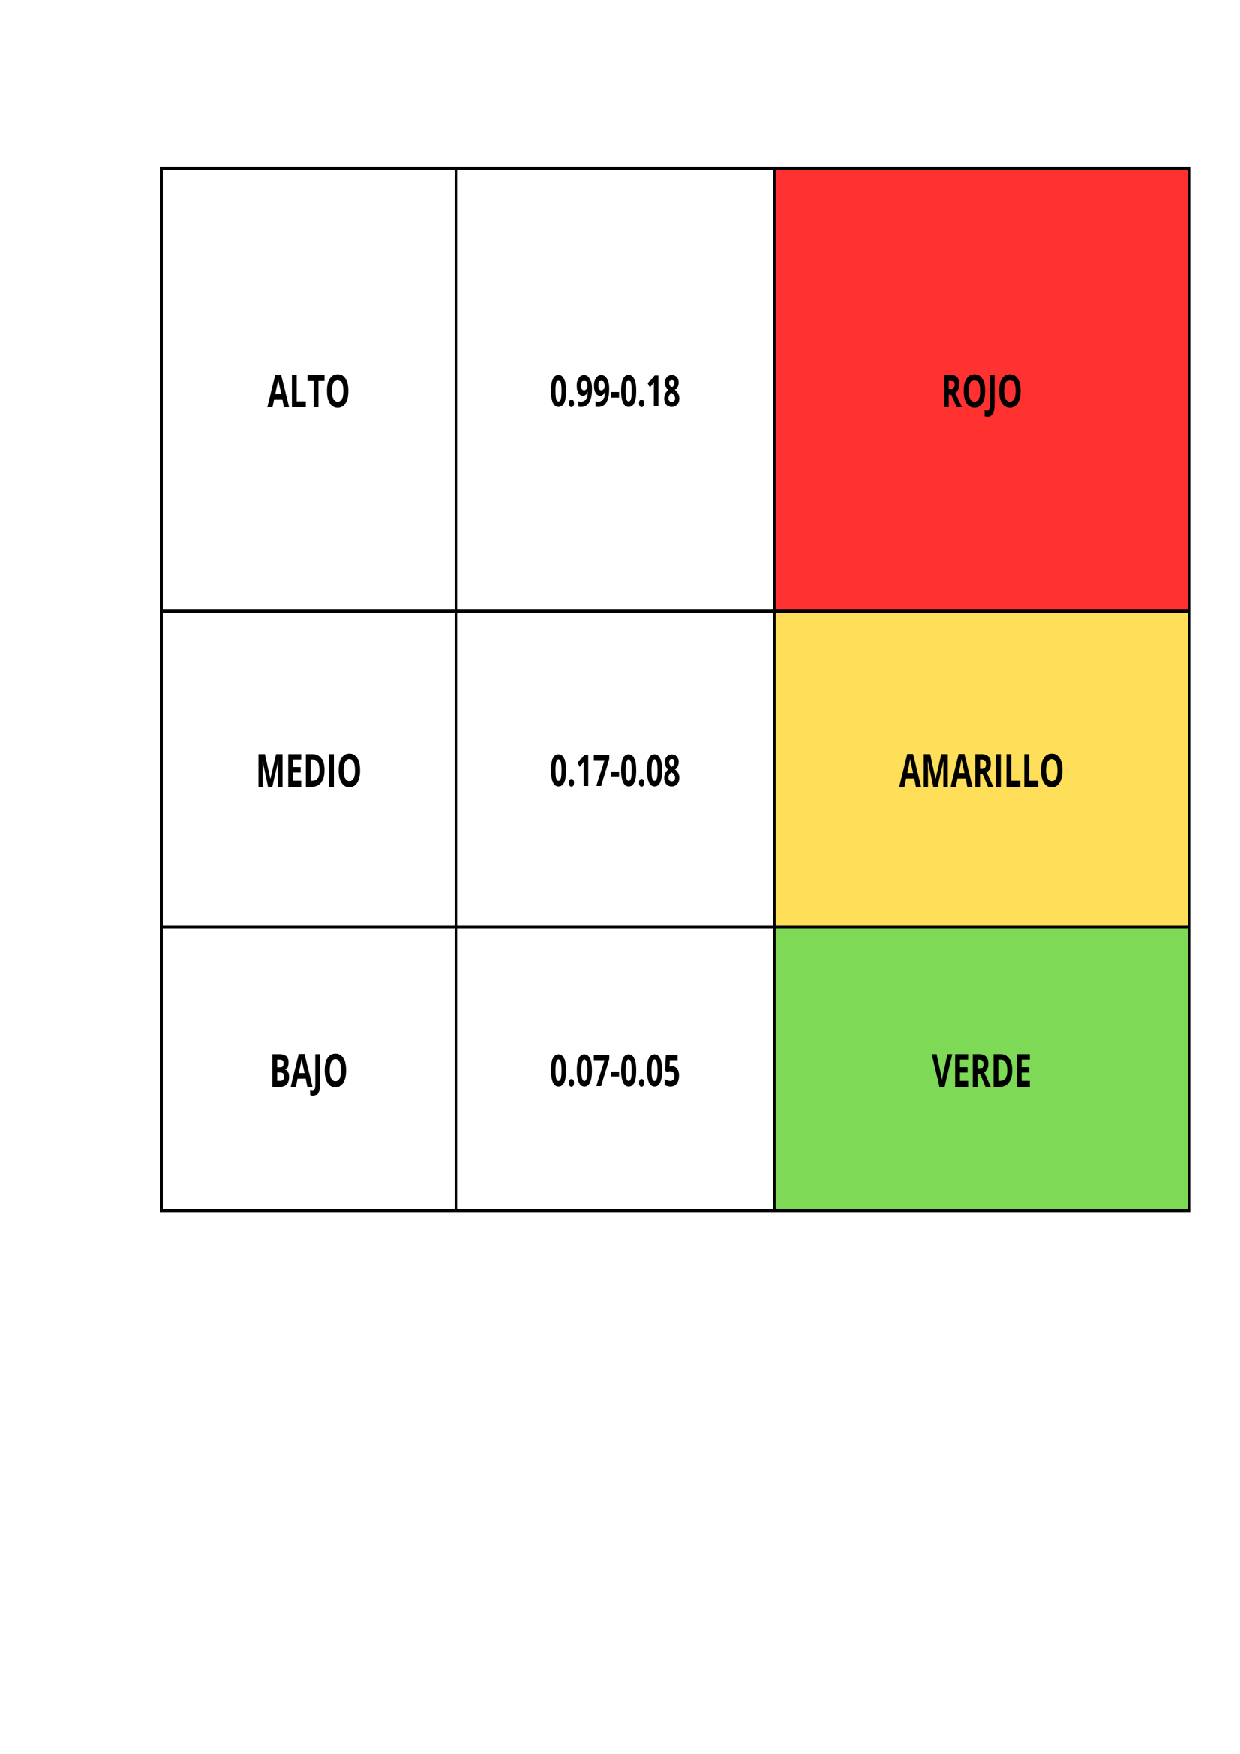
\includegraphics[trim = {20mm 40mm 20mm 25mm},clip,scale=0.25]{9/Img/nivelesRiesgos.pdf}
        \caption{Riesgos con diferentes niveles y colores para distinguir la gravedad y accione }
        \label{fig:bimanual}
    \end{figure}
    %
    \subsubsection{Riesgos internos}
    El riesgo se define como la posibilidad de que algo suceda o no suceda en otras palabras es la proximidad de un daño.\cite{H}
    %
    \begin{figure}[H]
        \centering
        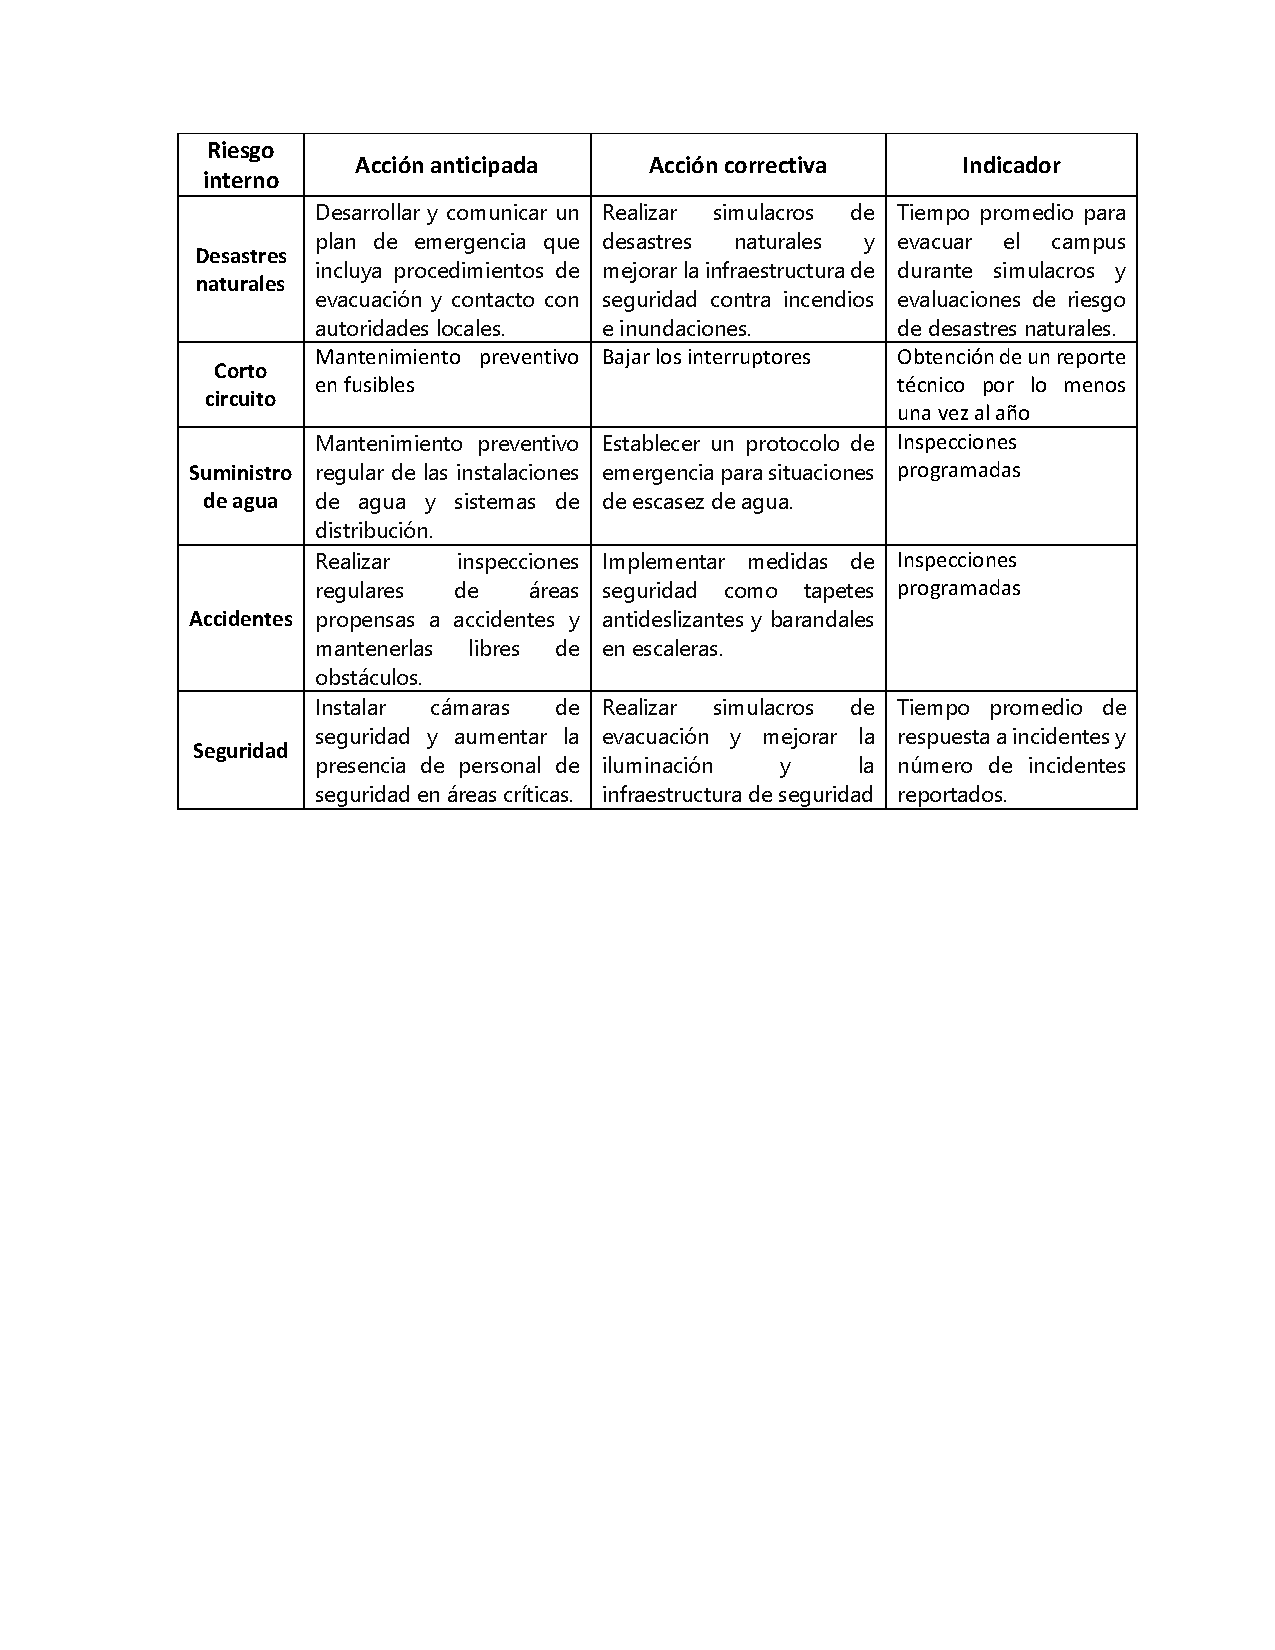
\includegraphics[trim = {20mm 40mm 20mm 25mm},clip,scale=0.30]{9/Img/riesgoInterno.pdf}
        \caption{Descripción de los riesgos Internos }
        \label{fig:bimanual}
    \end{figure}
    
    % 
    \subsubsection{Riesgos externos}
    % 
    Son  aquellos que provienen del entorno de una organización y que pueden influir o condicionar su operativa, pudiendo convertirse en amenazas para su desarrollo.\cite{H} 
    Estos riesgos pueden ser diversos y pueden provenir de diferentes fuentes, como por ejemplo, cambios en las condiciones económicas, cambios en la regulación gubernamental, desastres naturales, conflictos geopolíticos, entre otros.
    %
    \begin{figure}[H]
        \centering
        \includegraphics[trim = {20mm 40mm 20mm 25mm},clip,scale=0.30]{9/Img/riesgosExterno.pdf}
        \caption{Descripción de los riesgos Externos }
        \label{fig:bimanual}
    \end{figure}
    % 
    \subsubsection{Programa de actividades de prevención y auxilio}
    % 
    Es importante garantizar un programa de actividades para asegurar la seguridad y el cuidado de los empleados, así como para asegurar la continuidad de las actividades en situaciones de emergencia o desastres. Por lo tanto, estas medidas de precaución se implementan antes de que suceda cualquier incidente.
    % 
    \subsubsection{Plan de acción}
    Un plan de acción es una herramienta de planificación que establece la manera en que se organizará, orientará e implementará el conjunto de tareas necesarias para la consecución de objetivos y meta.\cite{NR}
    Es importante revisar y actualizar regularmente el plan de acción de emergencia, así como realizar simulacros periódicos para garantizar que todo el personal esté preparado y capacitado para actuar en caso de una emergencia.
    % 
    \begin{figure}[H]
        \centering
        \includegraphics[scale=0.1]{9/Img/accionesAnticipada.pdf}
        \caption{Descripción de las acciones anticipadas y correctivas ante un riesgo internos}
        \label{fig:mapa-itq}
    \end{figure}
    
    \begin{figure}[H]
        \centering
        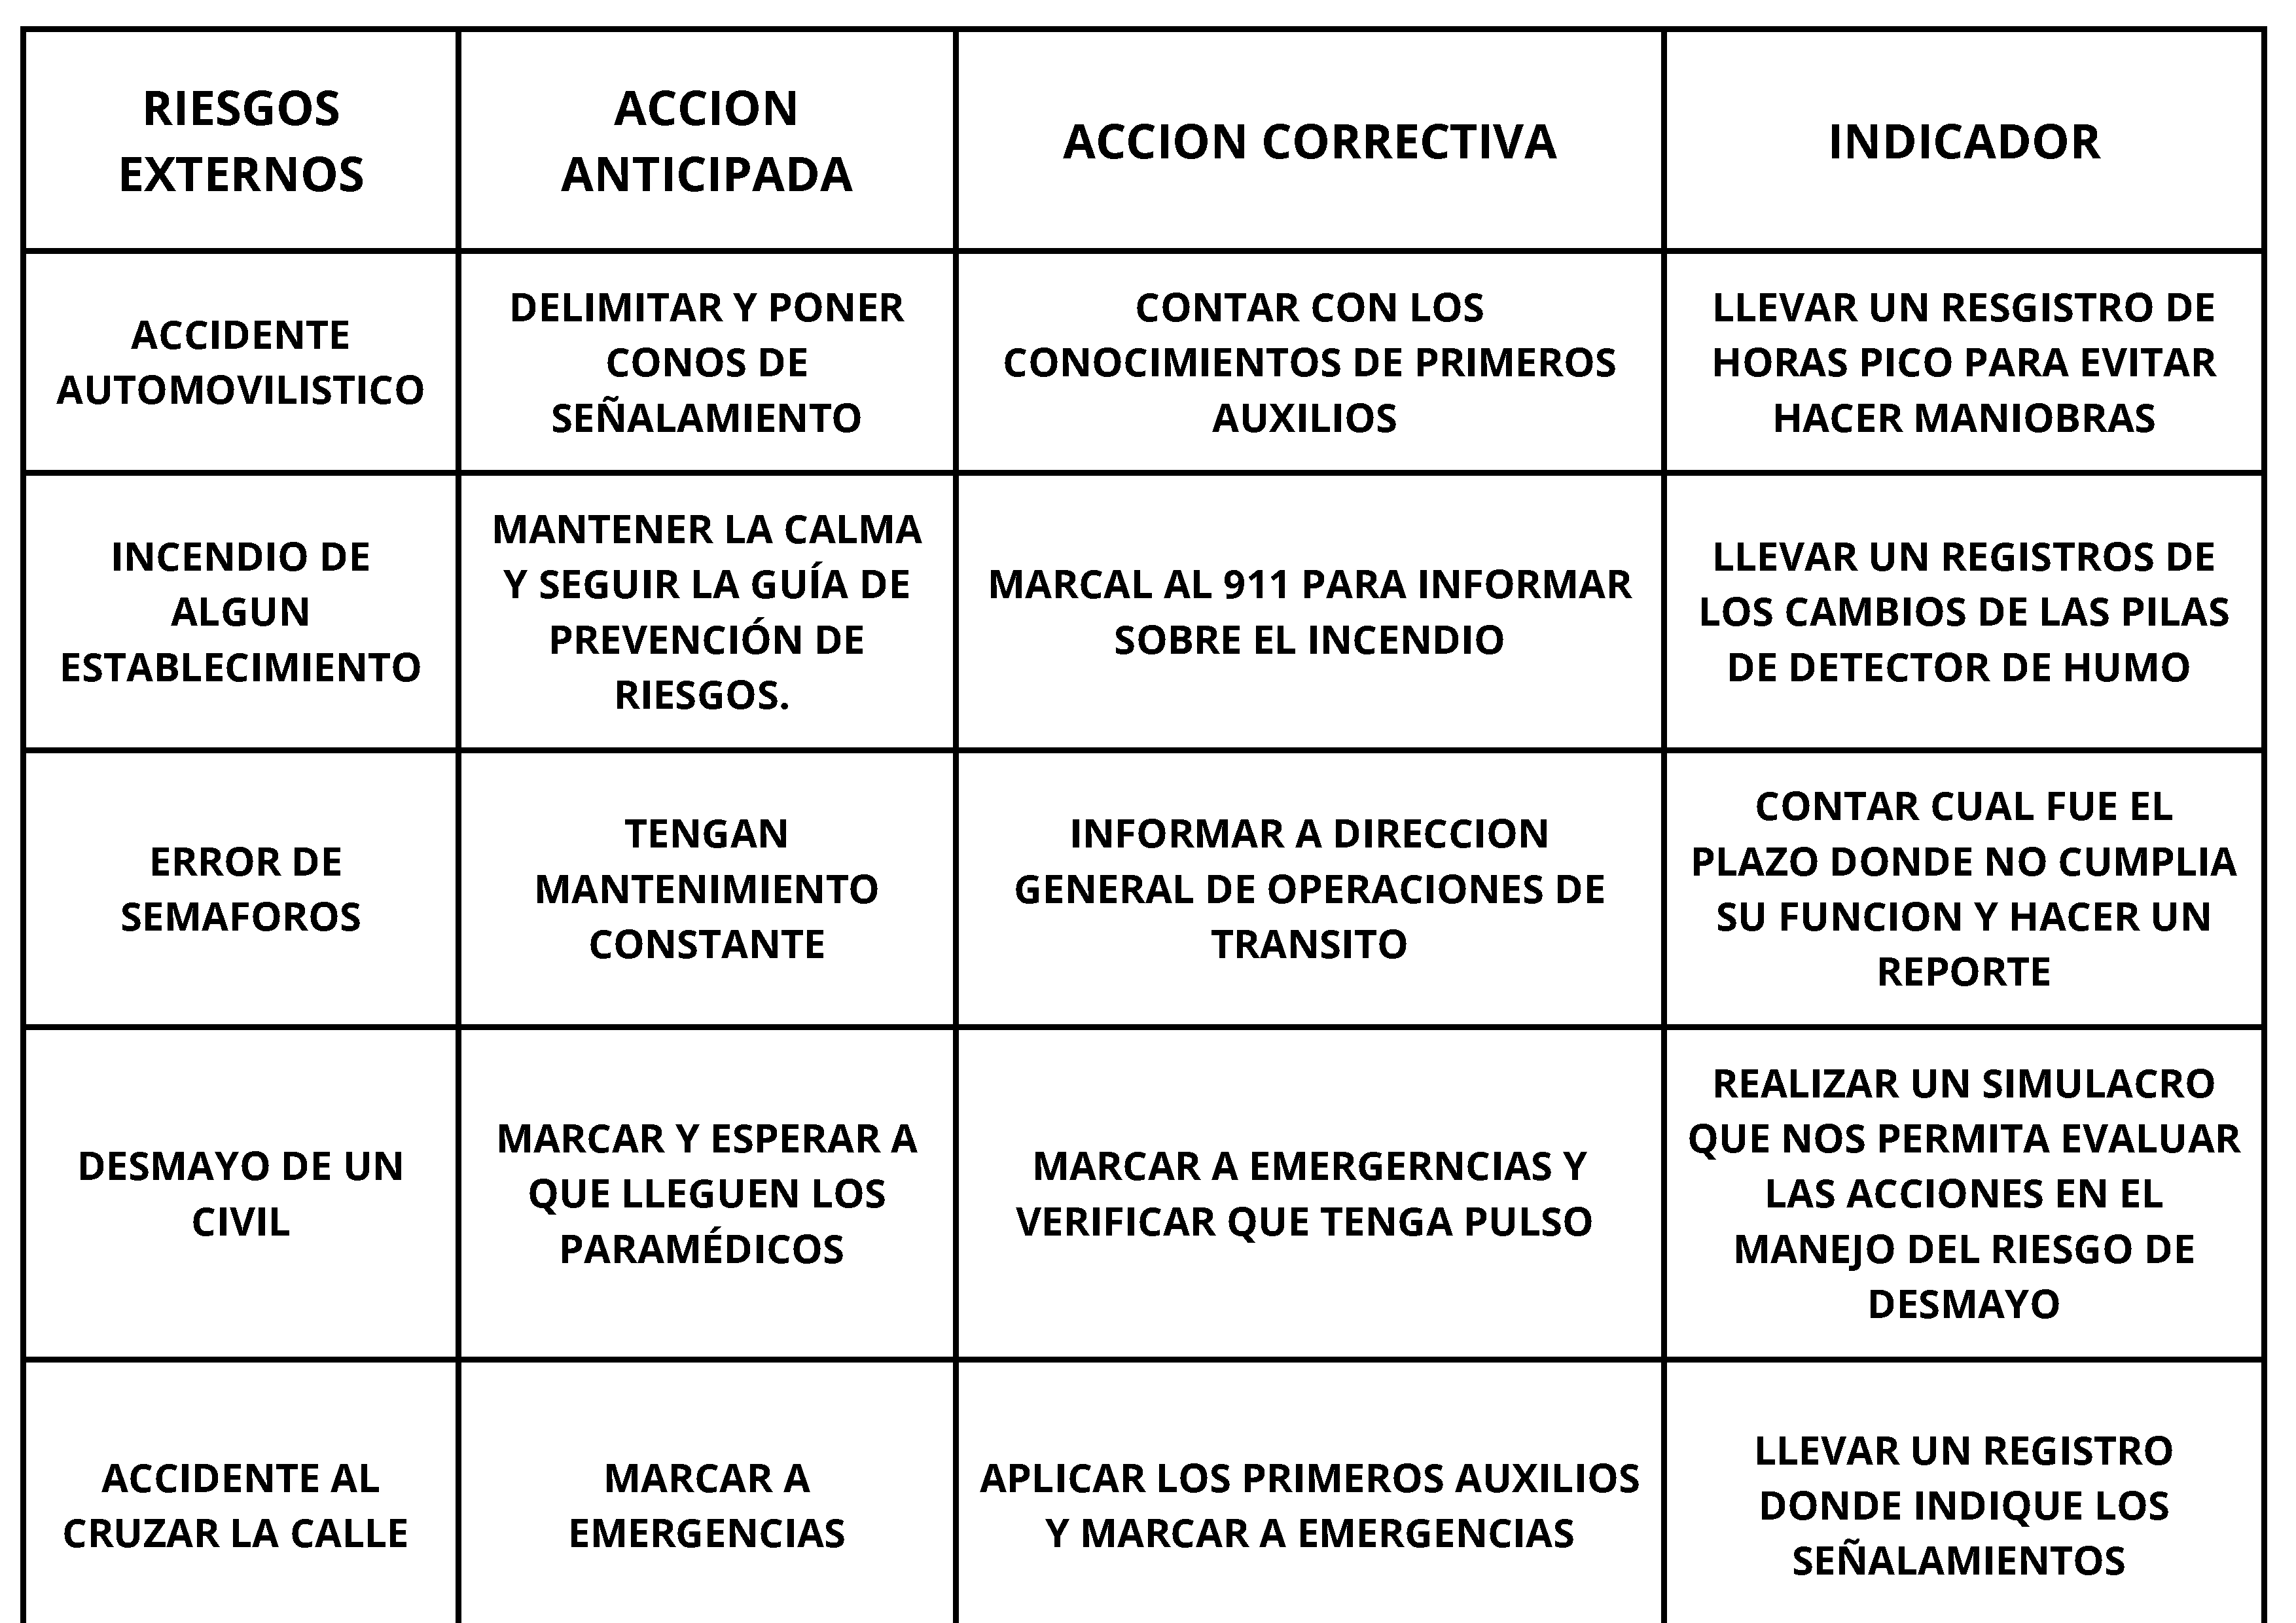
\includegraphics[scale=0.1]{9/Img/accionesAnticipadas.pdf}
        \caption{Descripcion de las acciones anticipadas y correctivas ante un riesgo internos}
        \label{fig:mapa-itq}
    \end{figure}
    % 
    % 
    \subsubsection{Identificación de capacidades}
    %
    \begin{table}[h]
        \centering
        \begin{tabular}{|c|c|c|}
        \hline
        \multicolumn{3}{c}{Horario}\\
        \hline
             No.& RECURSO& CANTIDAD \\
        \hline
             1 & EXTINTOR & 6\\
        \hline
             2 & BOTIQUÍN & 3\\
        \hline 
             3 & DETECTOR DE HUMO & 3\\
        \hline
             4 & LAMPARA DE EMERGENCIAS & 8\\
             \hline
        \end{tabular}
        \caption{Recursos en material de emergencias}
        \label{tab:riego}
    \end{table}
    %
    \subsubsection{Plano de localización de recursos}
    % 
    Es una herramienta de planificación que visualiza la ubicación de diversos recursos en relación con un proyecto o lugar específico.\cite{E}
    %
    \begin{figure}[H]
        \centering
        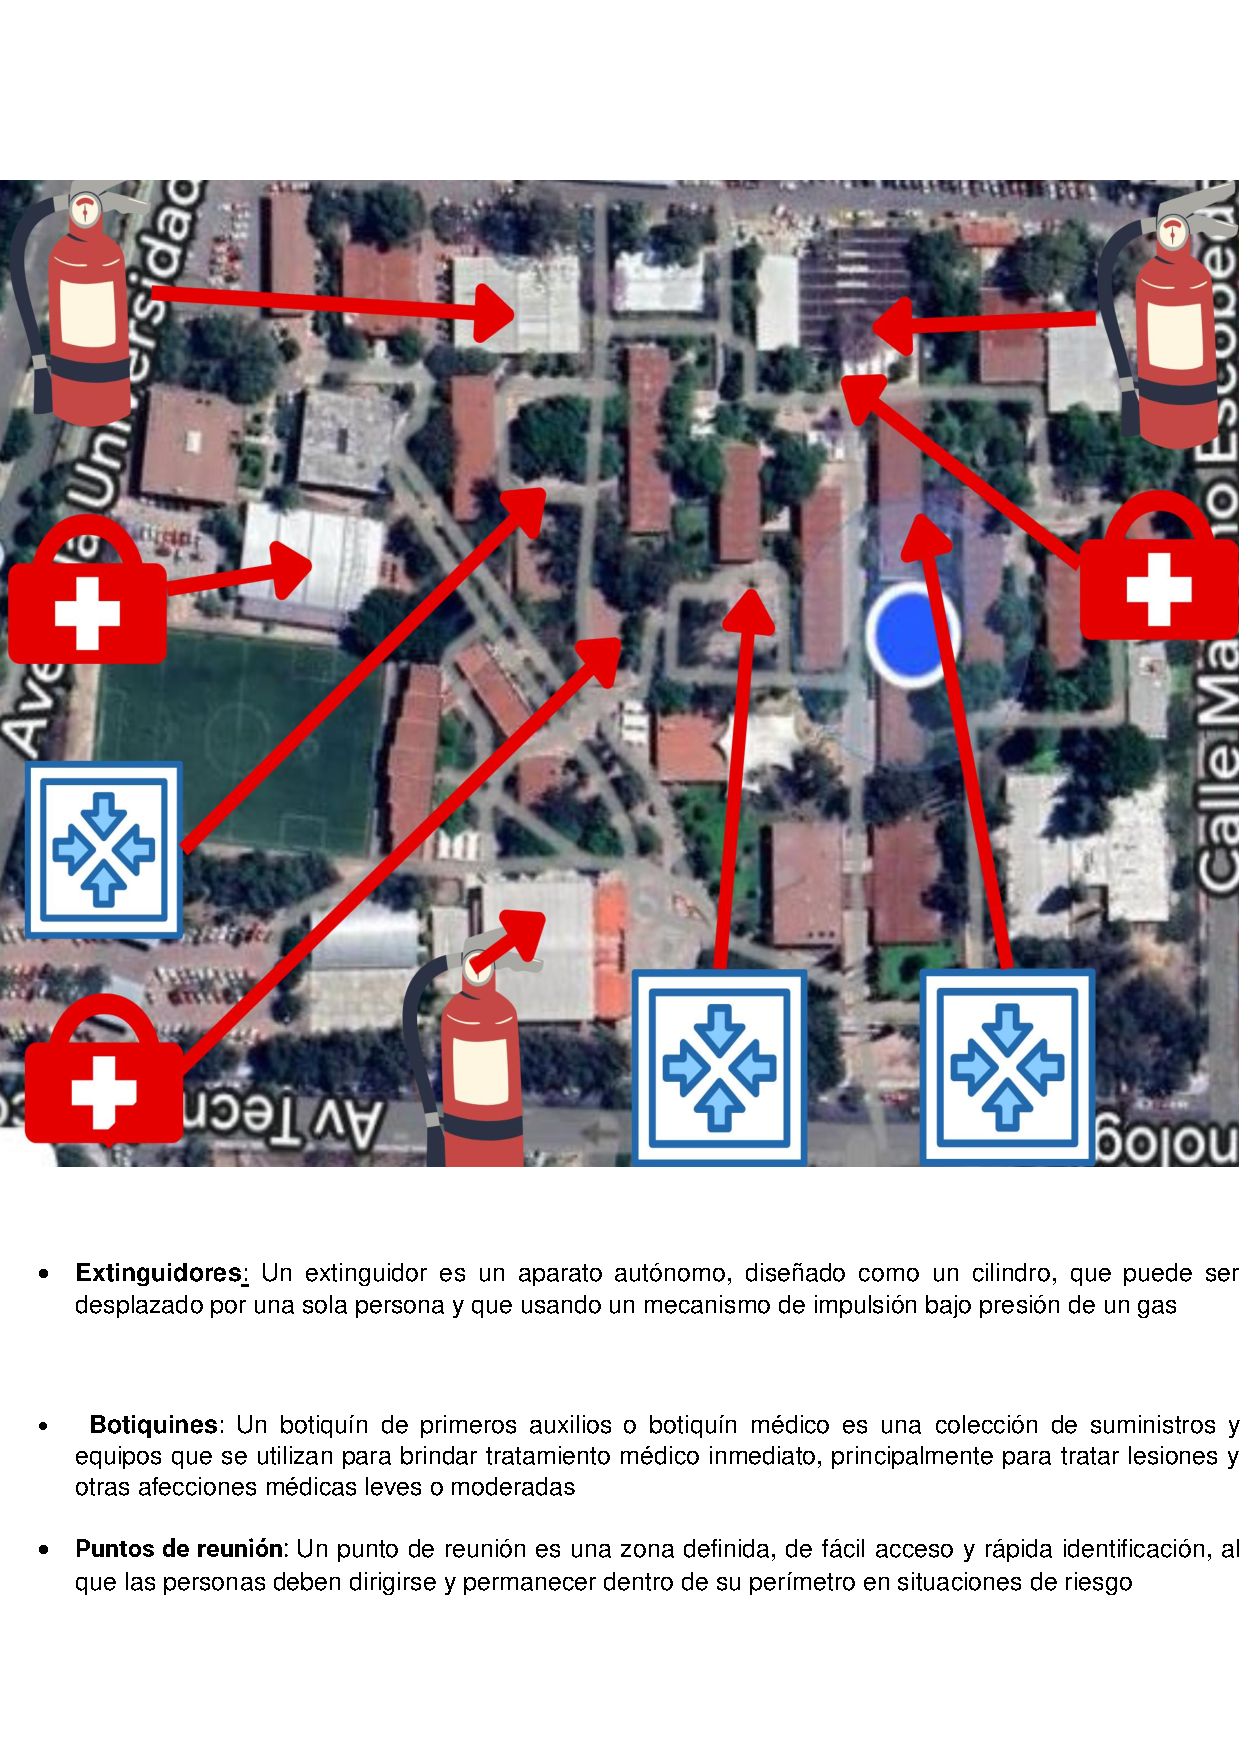
\includegraphics[scale=0.3]{9/Img/planoEstablecimiento.pdf}
        \label{fig:mapa-itq}
    \end{figure}
    % 
    \subsubsection{ Identificación de apoyos externos}
    %
    Son todos los procesos cuyo único propósito es asegurar el funcionamiento de los procesos de creación de valor y la propia marcha de la empresa.\cite{GP}
    % 
    \begin{figure}[H]
        \centering
        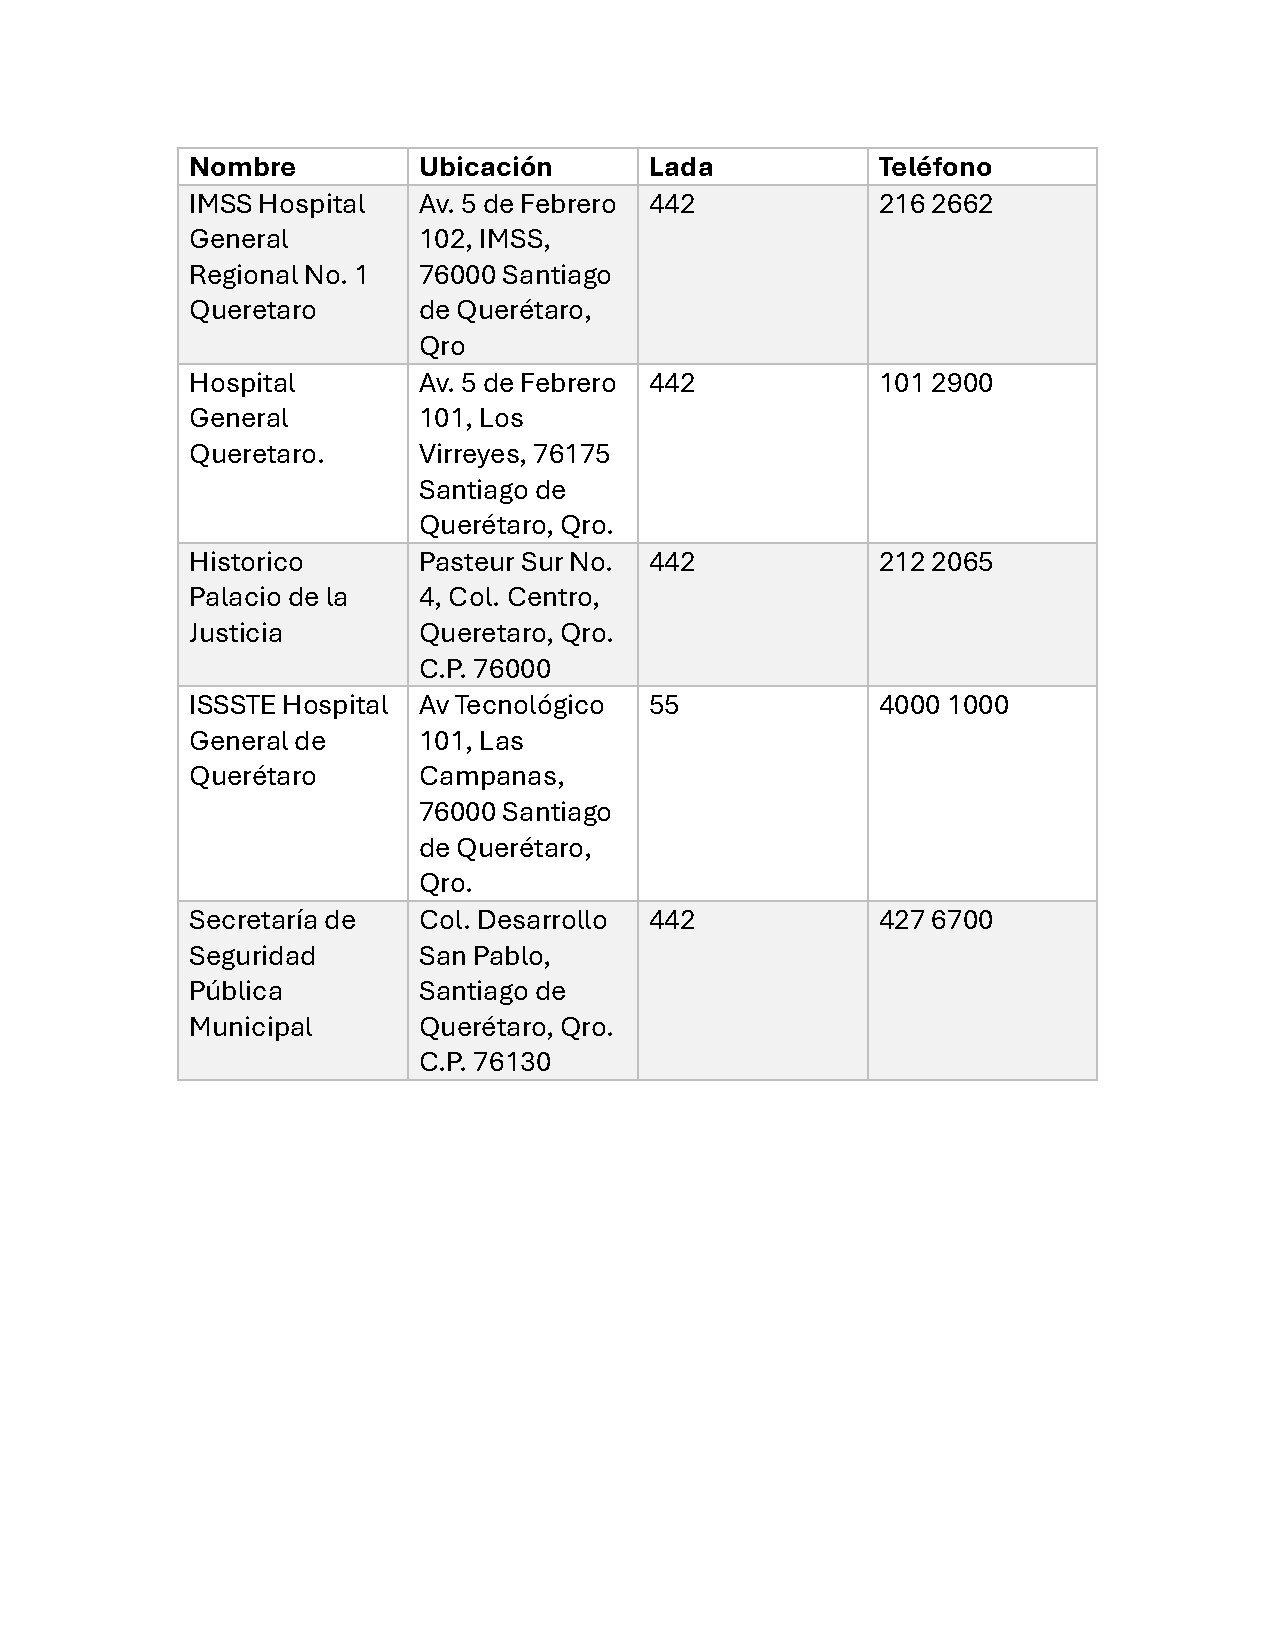
\includegraphics[scale=0.5]{9/Img/apoyosExternos.pdf}
        \caption{Lugares que servirán de apoyo en un situación de emergencia.}
        \label{fig:mapa-itq}
    \end{figure}
    % 
    % 
    %
    % 
    \subsubsection{Identificación de puntos de reunión}
    
    \begin{figure}[H]
        \centering
        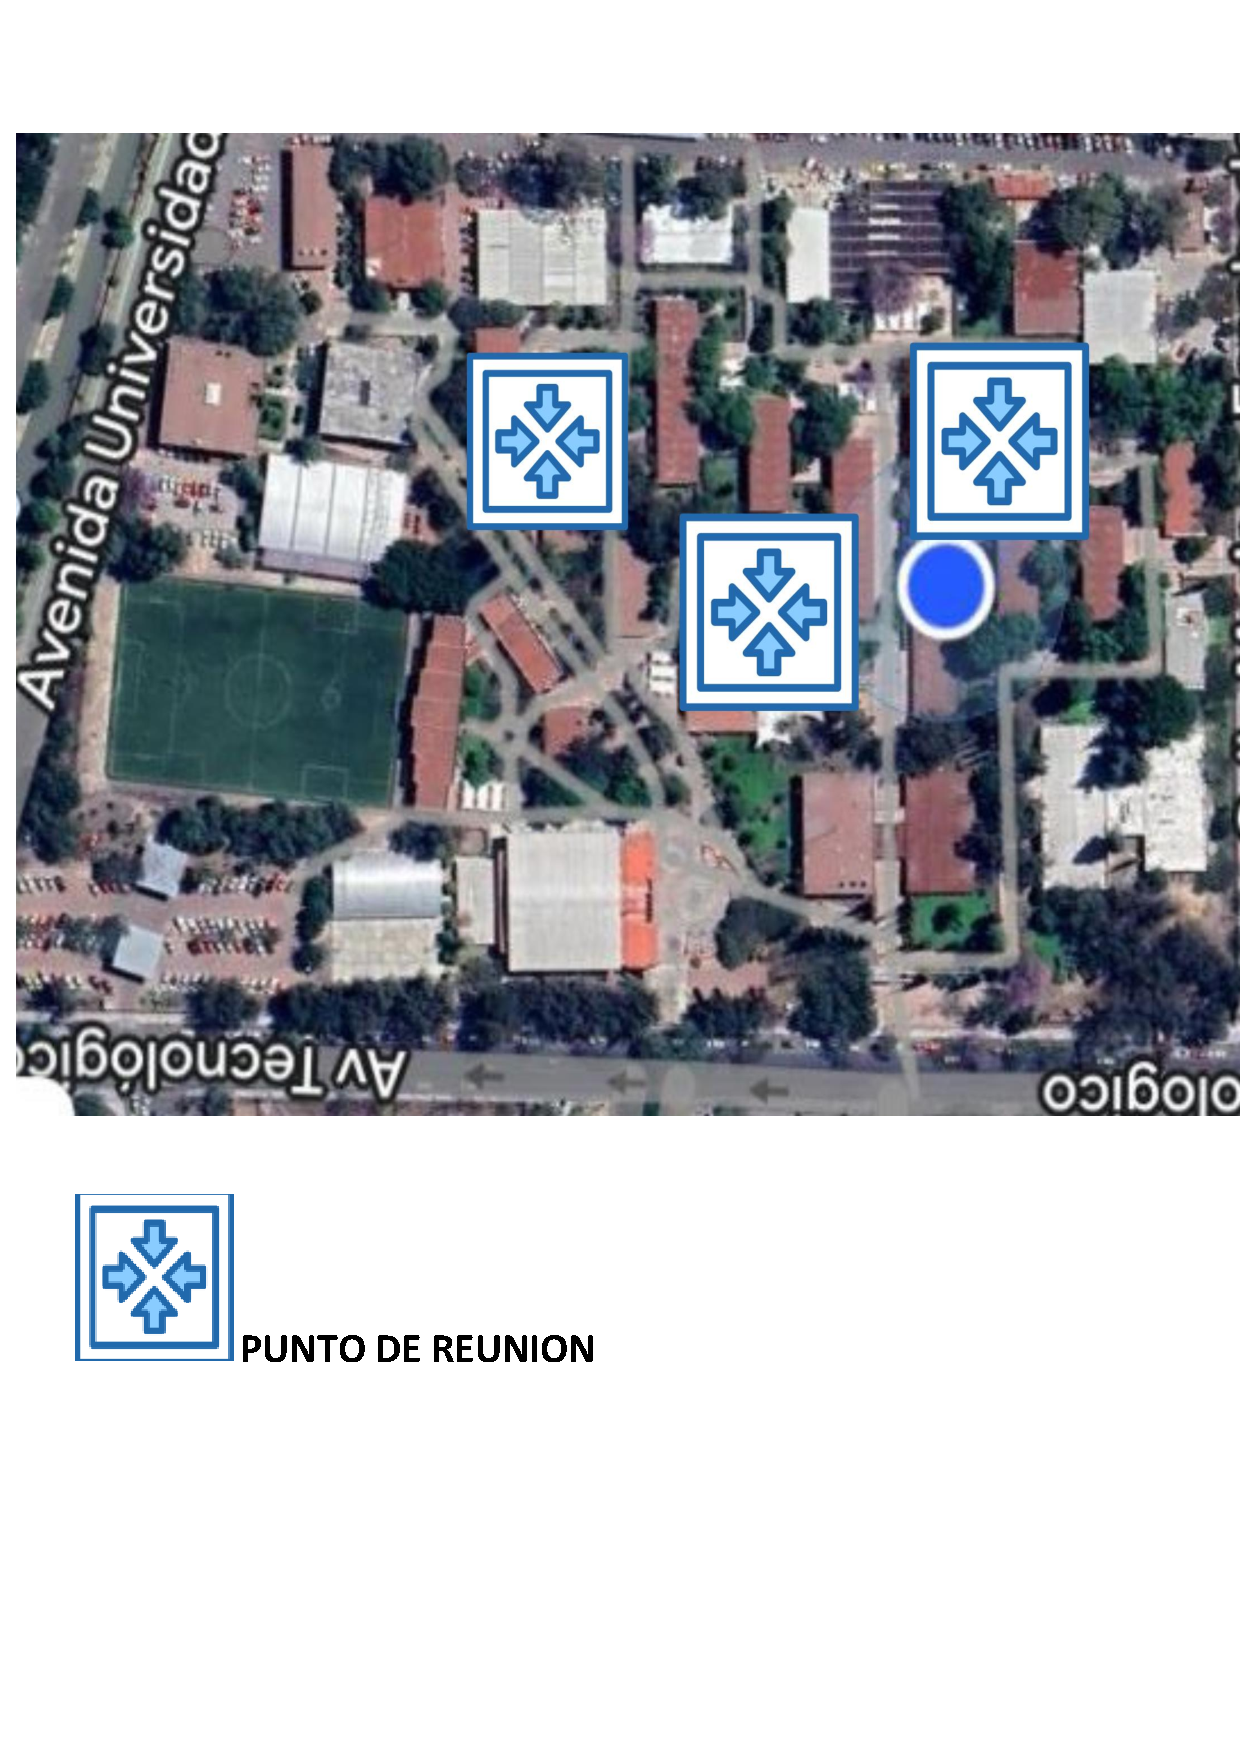
\includegraphics[trim = {40mm 60mm 20mm 21mm},clip,scale=0.35]{9/Img/puntoReunion.pdf}
        \caption{Zona segura en caso de una evacuación de emergencia.}
        \label{fig:puntosDeReunión}
    \end{figure}
    % 
    \subsubsection{Brigada de evacuación}
    %
    La brigada de evacuación es un pilar fundamental en la gestión de emergencias ya que su accion rápida y coordenada puede salvar vidas en momentos críticos, es fundamental que las organizaciones cuenten con un equipo de brigadas capacitados y comprometido con la seguridad de todos.
    Debe de contar con un plan detallado de accion, conocer las rutas de evacuación, tener conocimiento sobre Primeros auxilios.
    %
    \begin{figure}[H]
        \centering
        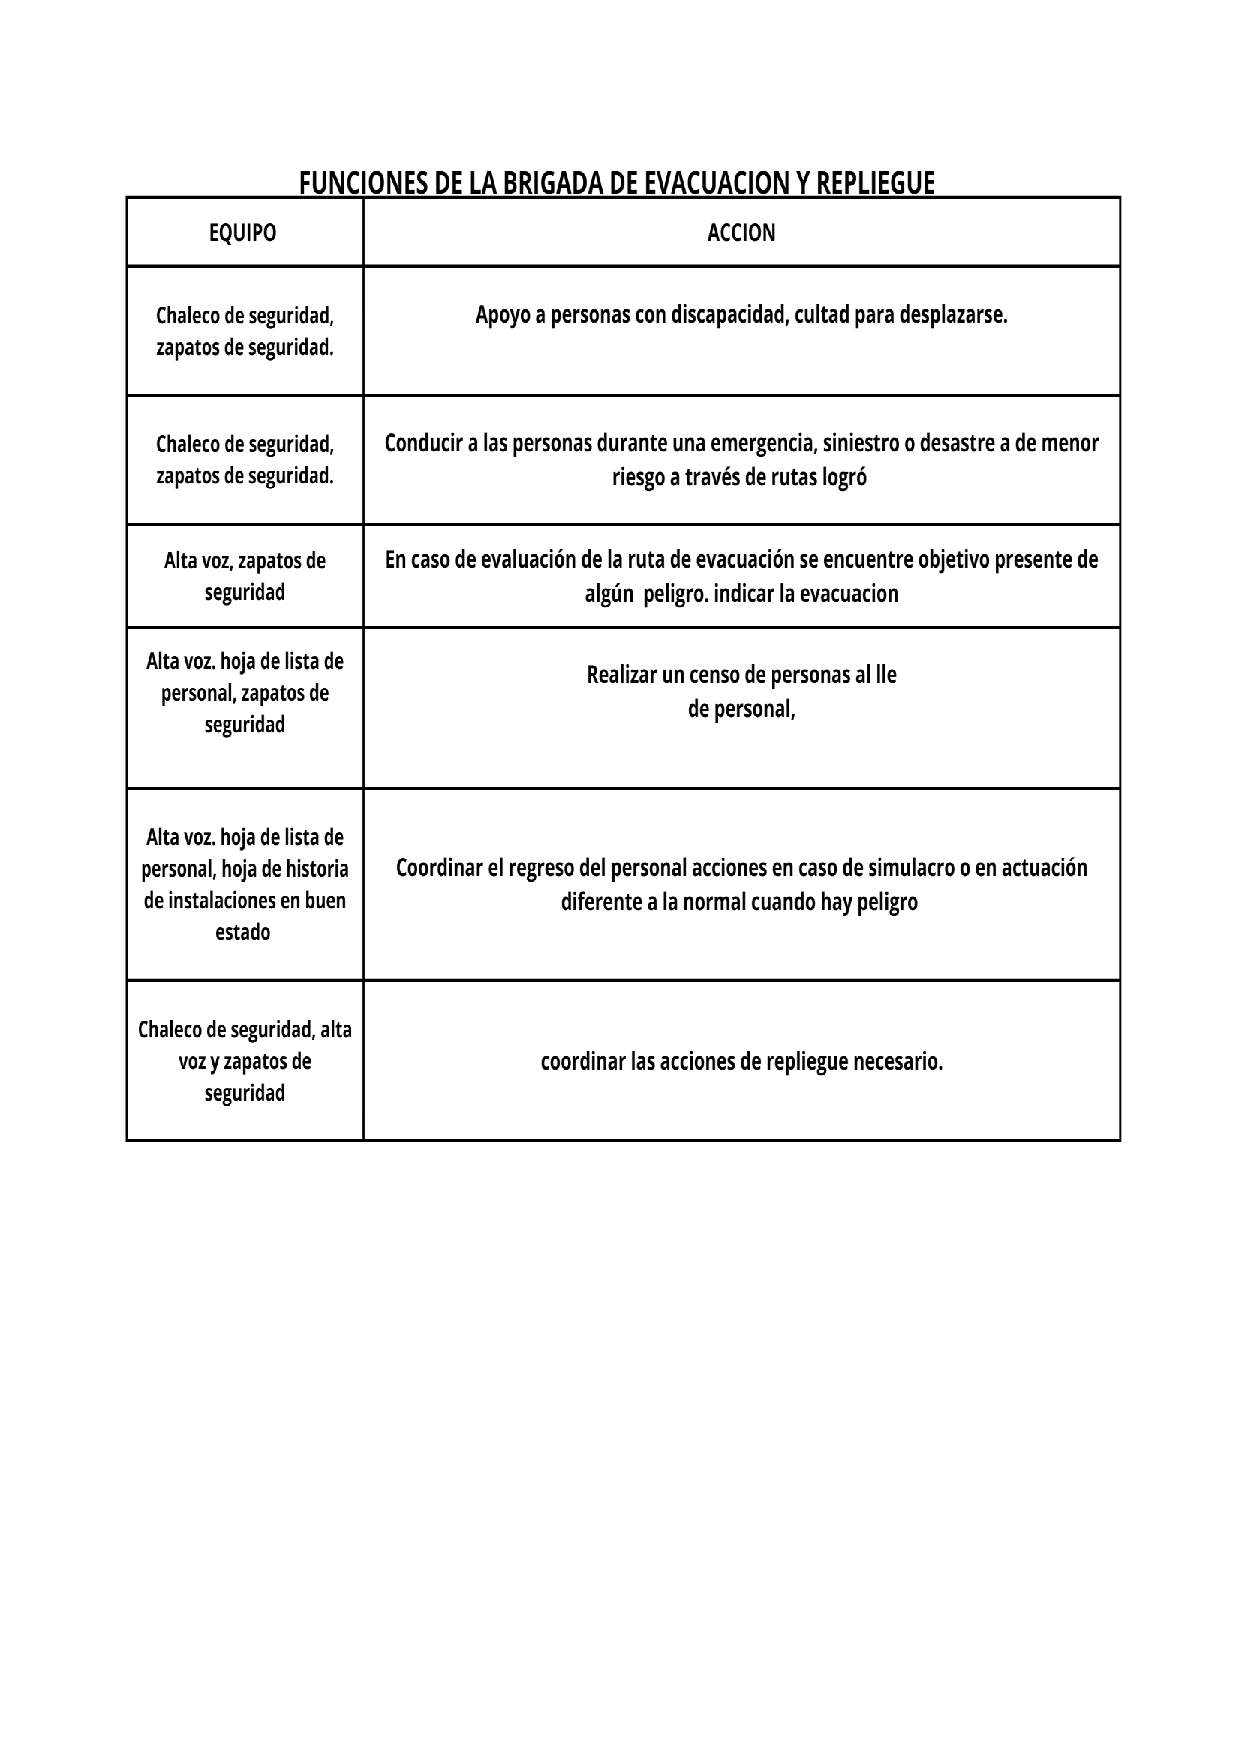
\includegraphics[trim = {15mm 35mm 20mm 45mm},clip,scale=0.5]{9/Img/brigadaEvacuacioon.pdf}
        \caption{Acciones asignadas a cada integrante del equipo de trabajo en caso de una evacuación de emergencia o repliegue.}
        \label{fig:brigada}
    \end{figure}
    %
    \subsubsection{Directorio de telefónicos de emergencia}
    % 
    El directorio telefónico de emergencia es una herramienta crucial para garantizar la seguridad y el bienestar de la comunidad en situaciones de crisis. Contar con los números de teléfono de servicios de emergencia como la policía, los bomberos, la ambulancia, entre otros, permite una respuesta rápida y eficaz ante cualquier situación de emergencia que pueda surgir.
    %
    
    \begin{figure}[H]
        \centering
        
\includegraphics[scale=0.25]{9/Img/emergencias.pdf}
        \caption{Números de emergencia de los bomberos más próximos a la ubicación el posible riesgo}
    \end{figure}
    % 
    % 
    \begin{figure}[H]
        \centering
        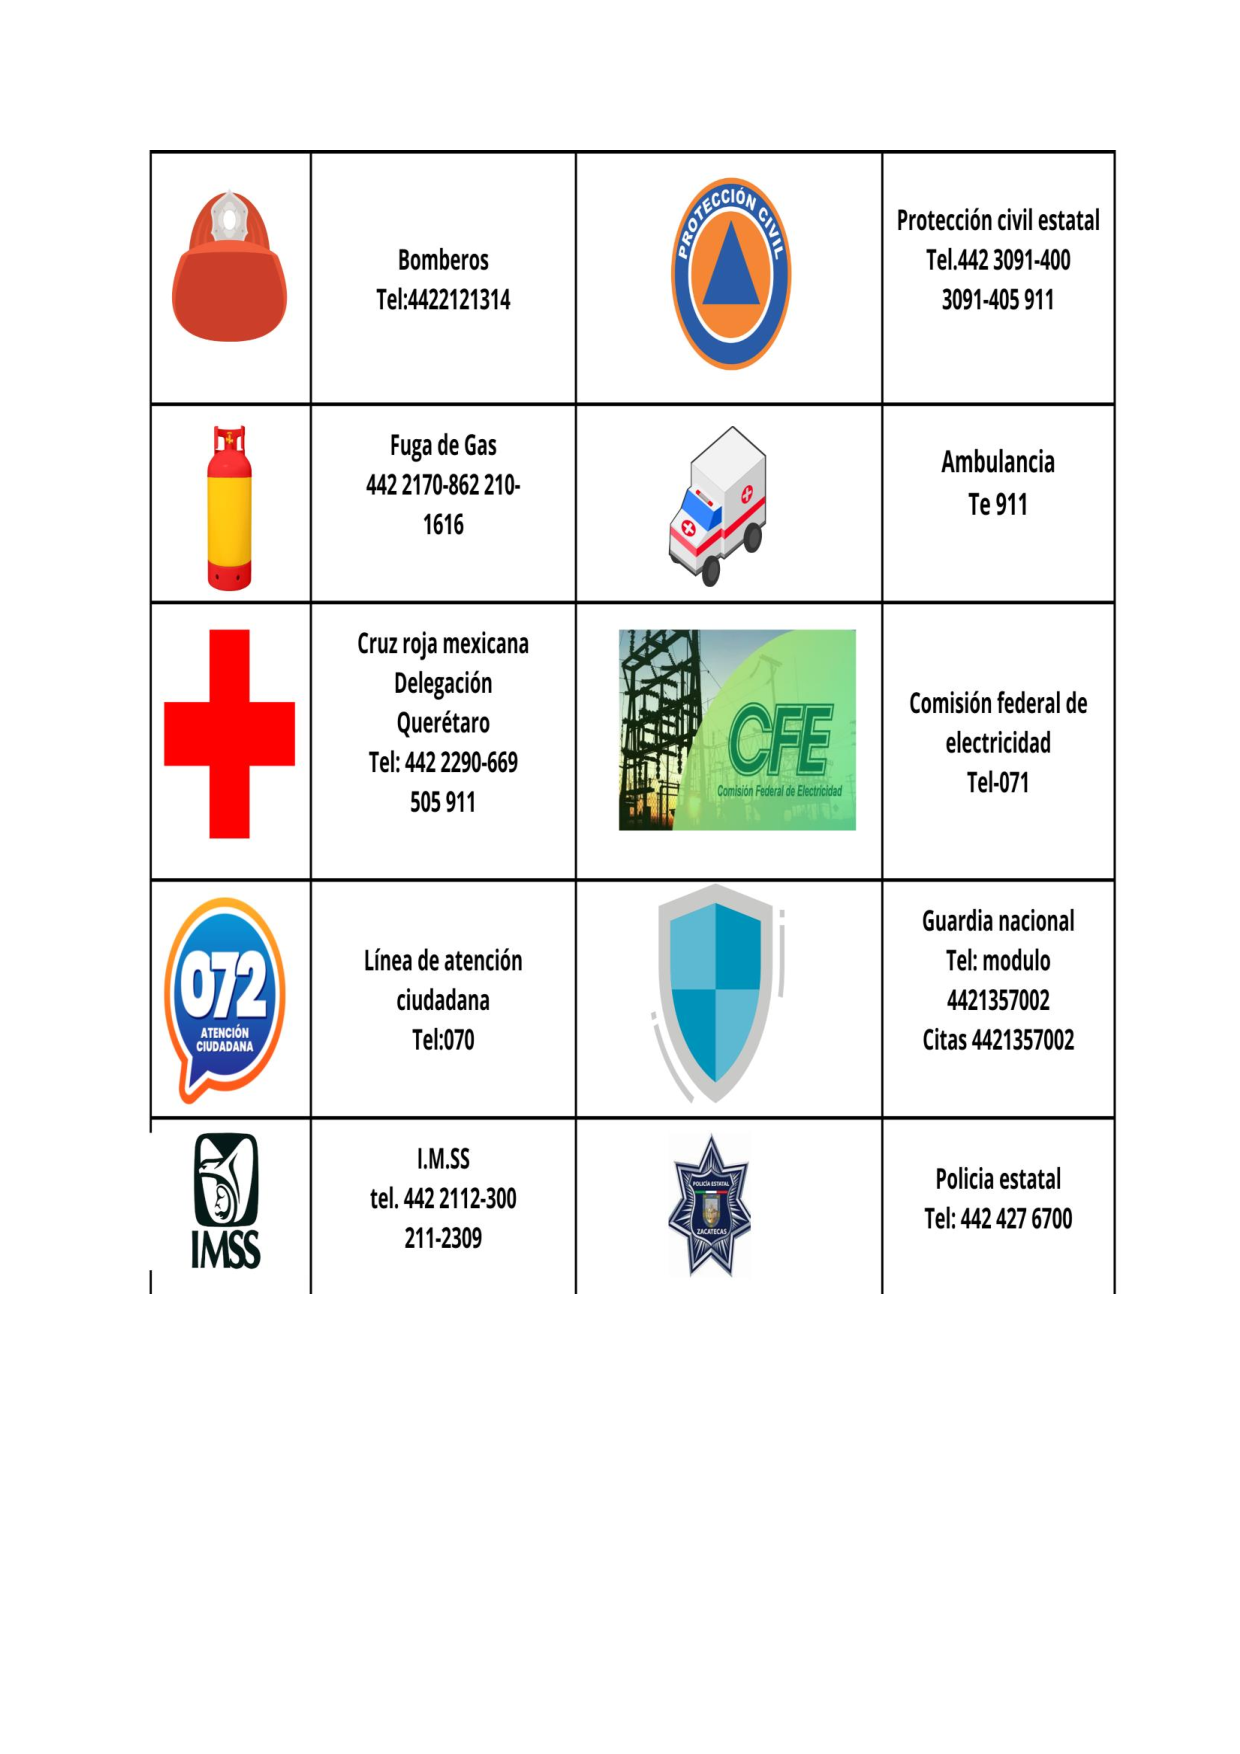
\includegraphics[scale=0.45]{9/Img/numeroEmergencia.pdf}
        \caption{Números de emergencia de los bomberos más próximos a la ubicación el posible riesgo}
    \end{figure}
    %
    
    Nombre Comercial: Instituto Tecnológico De Querétaro (ITQ) 
    
     Objetivo: Identificar y analizar los accidentes internos y externos que se realicen dentro del Tecnológico Nacional De Querétaro, capacitando el personal en un tiempo establecido.\\
    Datos Generales Del Establecimiento\\ 
    Ubicación: Avenida Tecnológico, esquina General Mariano Escobedo, Colona Centro 76000 Querétaro\\
    Institución: Instituto Tecnológico De México campus Querétaro.\\
    Representante Legal: Ing. Ramon Soto Arriola\\  
    Teléfono: 44-22-27-44-00\\ 
    Sitio Web: queretaro.tecnm.mx\\ 
    
    \begin{table}[h]
        \centering
        \caption{HORARIO DE ATENCION}
        \begin{tabular}{|c |c |}
        \hline
        \multicolumn{2}{c}{Horario}\\
        \hline
             LUNES& 7 a.m-10 p.m  \\
        \hline
             MARTES& 7 a.m - 10:30 pm\\
        \hline
             MIERCOLES& 7 a.m-10 p.m \\  
        \hline
             JUEVES& 7 a.m-10 p.m\\
        \hline
             VIERNESS& 7 a.m-10 p.m\\
        \hline
             SABADO& CERRADO\\
        \hline
             DOMINGO& CERRADO\\
        \hline     
        \end{tabular}
        \label{tab:riego}
    \end{table}
    %
    \subsection{Análisis de los métodos, materiales, herramientas e instalación utilizada en la ejecución del ensamble de un circuito electrónico}
    
    \subsubsection{Verificación}
    %
    Con base a las muestras realizadas por el analista y el operador, donde se fue realizando paso a paso con el apoyo de una guía el ensamble fue realizado con materiales y procesos de las nuevas técnicas de estudio, tomando en cuenta las Metodologías empleadas en este proyecto. Así se establece el final del circuito.
    %
    \begin{table}[h]
        \centering
        \caption{Riesgos con diferentes niveles y colores para distinguir la gravedad y acciones}
        \begin{tabular}{|c| c|}
        \hline
        \multicolumn{2}{c}{REFERENCIAS}\\
        \hline
             Nombre Operador & Collman Granados Joseph Iker  \\
        \hline
             Numero de control& 22140906  \\
        \hline
              Genero & Masculino \\
        \hline
             Nombre Analista& Fentanes Hernandez Ana Karen\\
        \hline
              Numero de control & 22140957\\
        \hline
            Genero & Femenino\\   
        \hline 
            Departamento & Industria\\
        \hline
            Maestro&  Luis Alberto Angeles\\
        \end{tabular}
        \label{tab:INFORMACION GENERAL}
    \end{table}
    %
    Al finalizar el proceso del ensamble el operador   hará un movimiento en el potenciómetro circularmente para verificar las lecturas,  posteriormente esto verificara que el manual funciono correctamente y concluir con el armado.  
    %
    \begin{figure}[H]
        \centering
        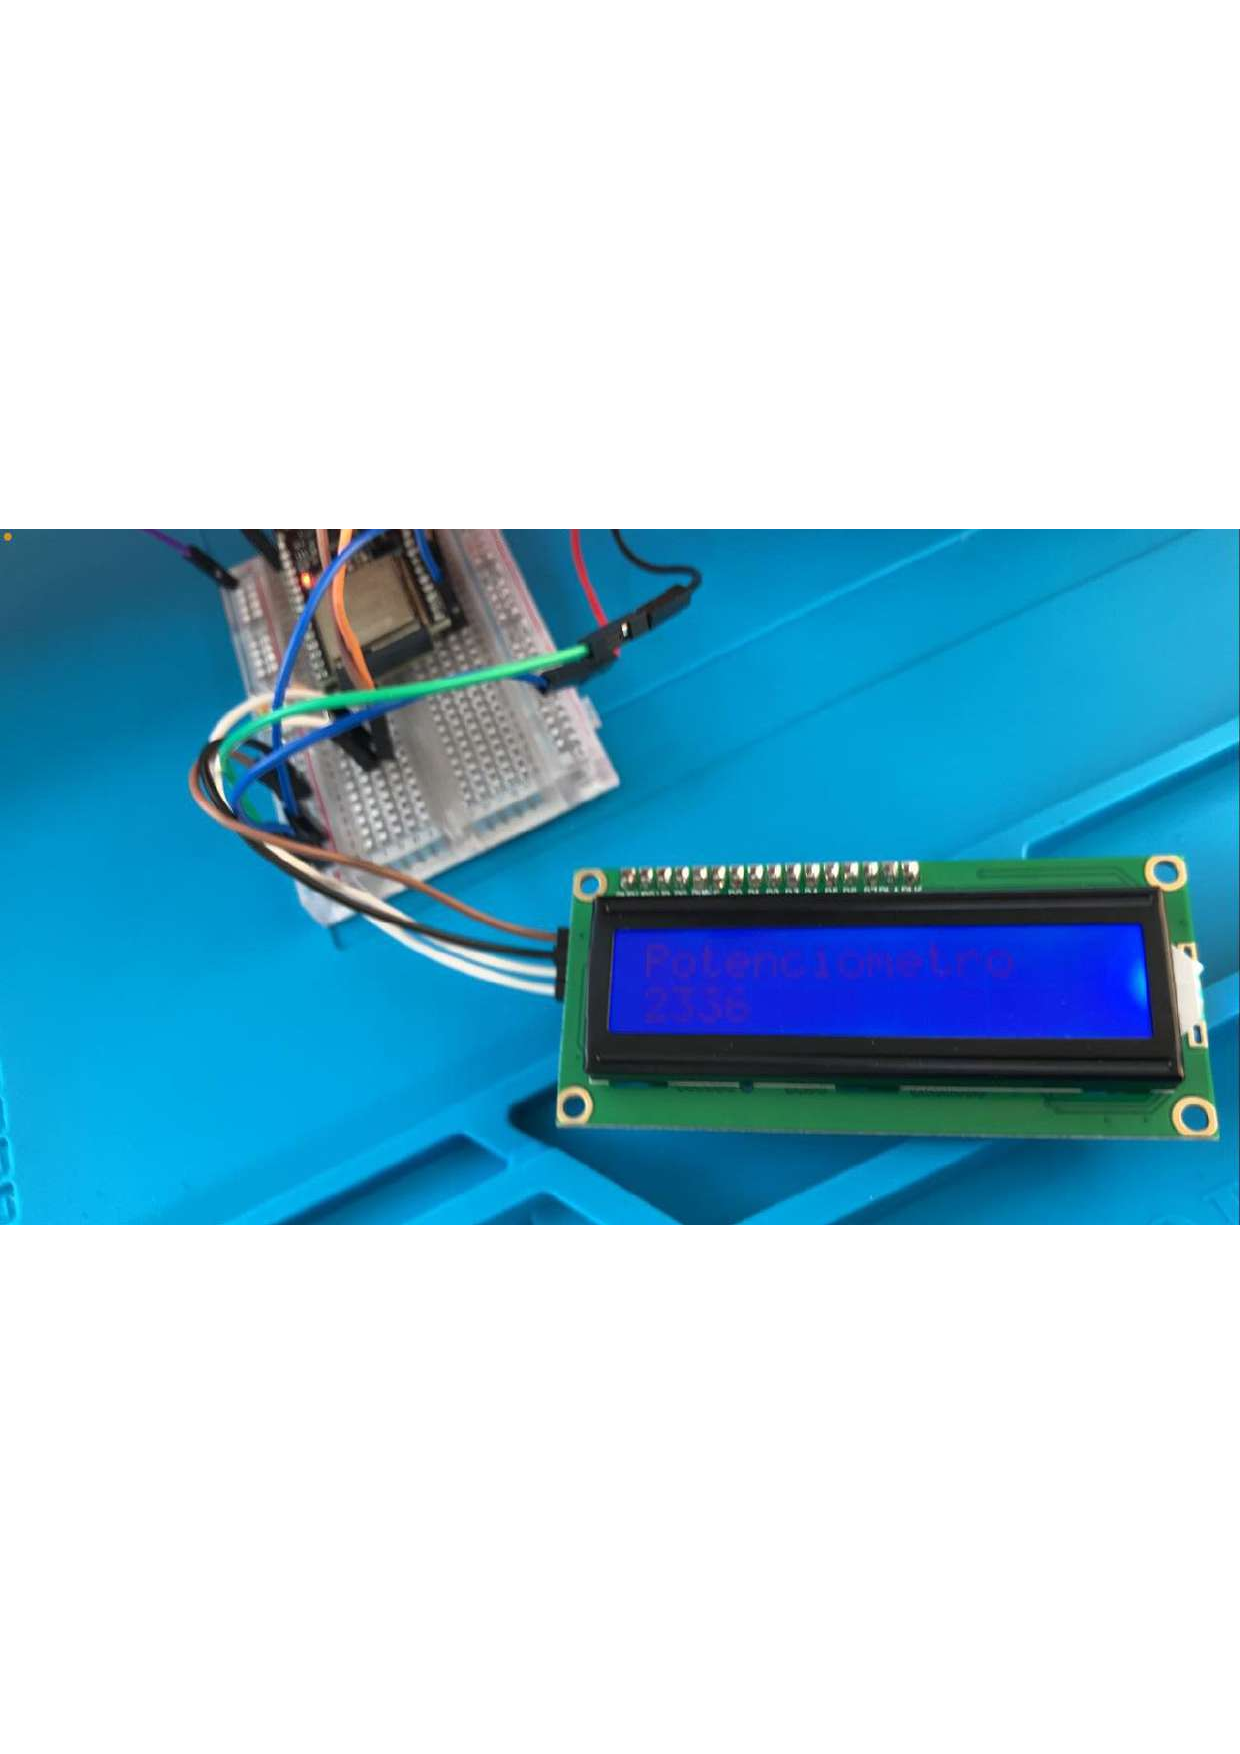
\includegraphics[scale=0.3]{9/Img/lectura.pdf}
        \caption{Números de emergencia de los bomberos más próximos a la ubicación el posible riesgo}
    \end{figure}
    % 
    \subsubsection{Desarrollo del sistema de tiempos predeterminado}
    % 
    \begin{figure}[H]
        \centering
        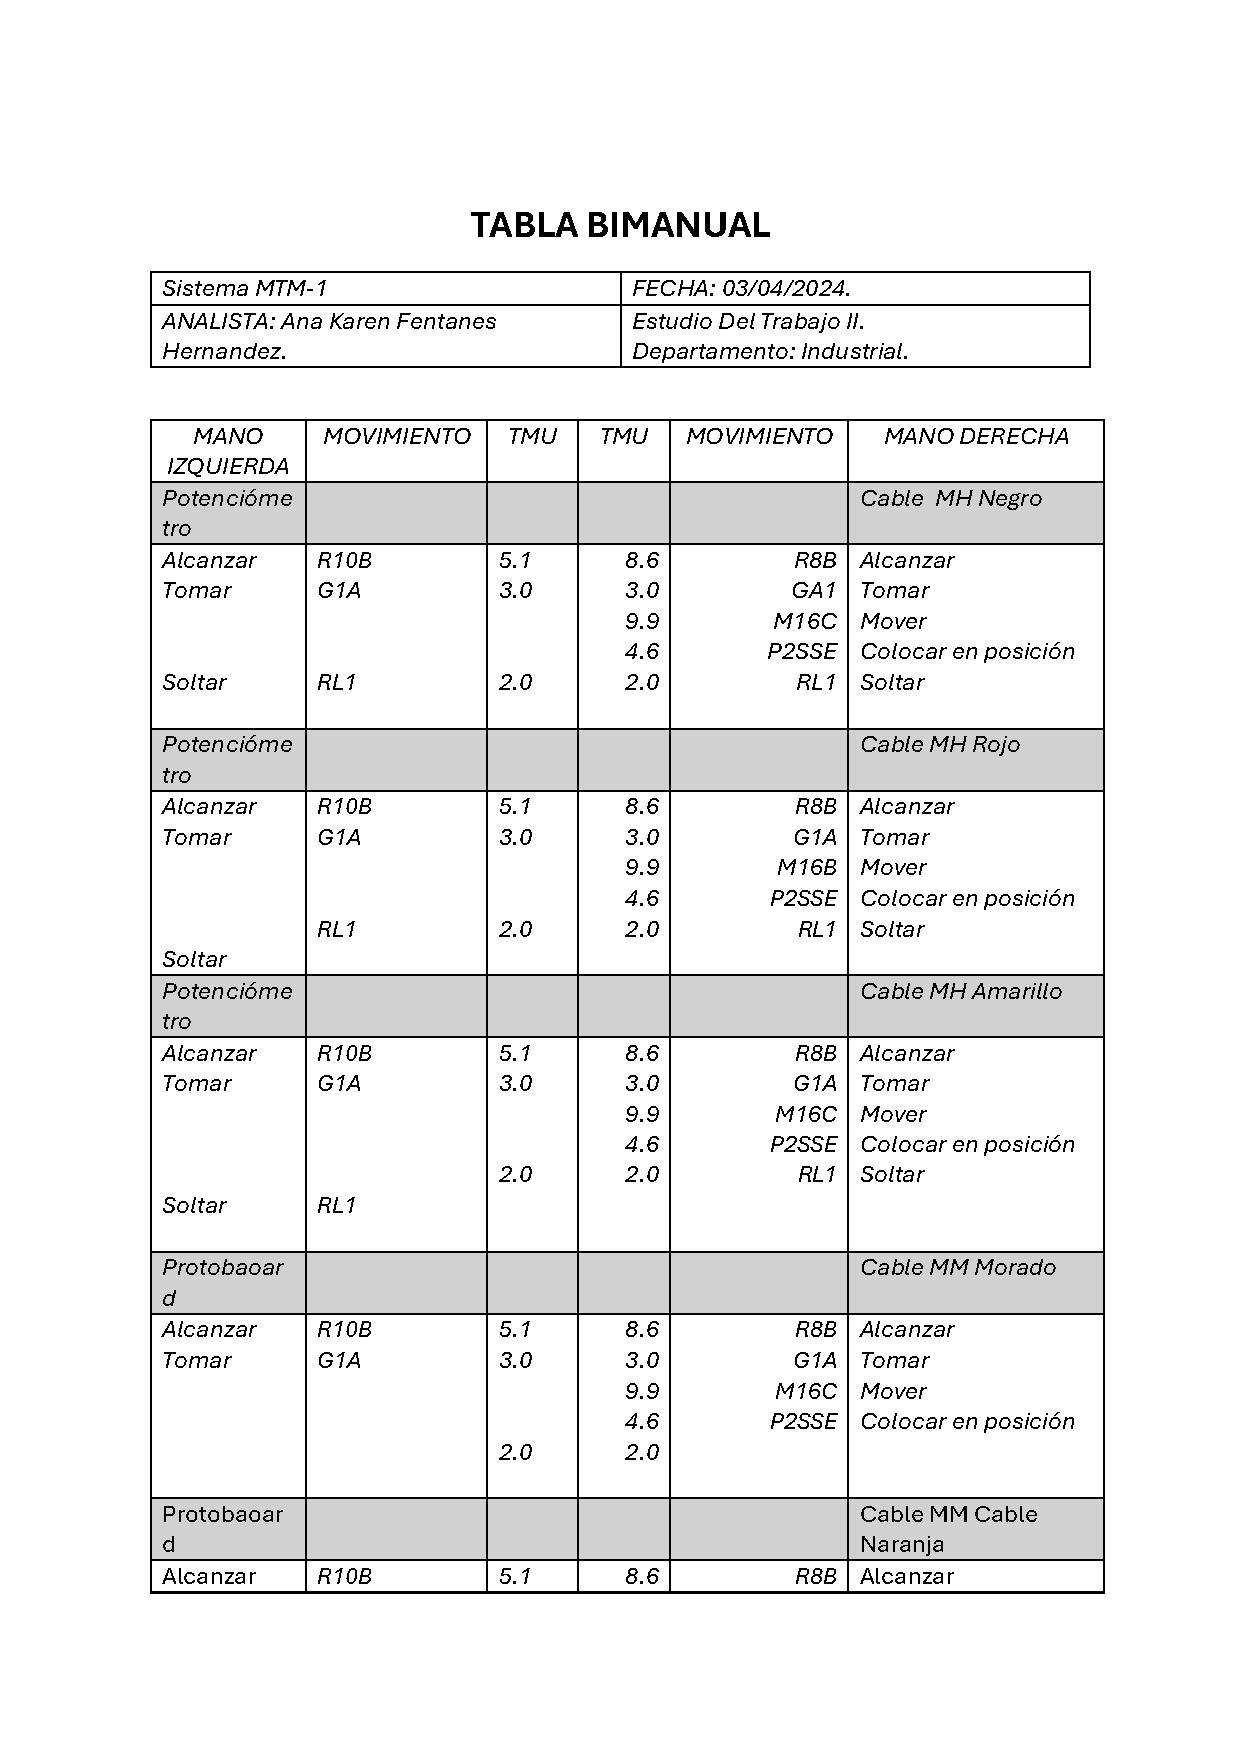
\includegraphics[trim = {40mm 60mm 20mm 21mm},clip,scale=0.35]{9/Img/tablaMtmUno.pdf}
        \label{fig:Mtm}
    \end{figure}
    %
    \begin{figure}[H]
        \centering
        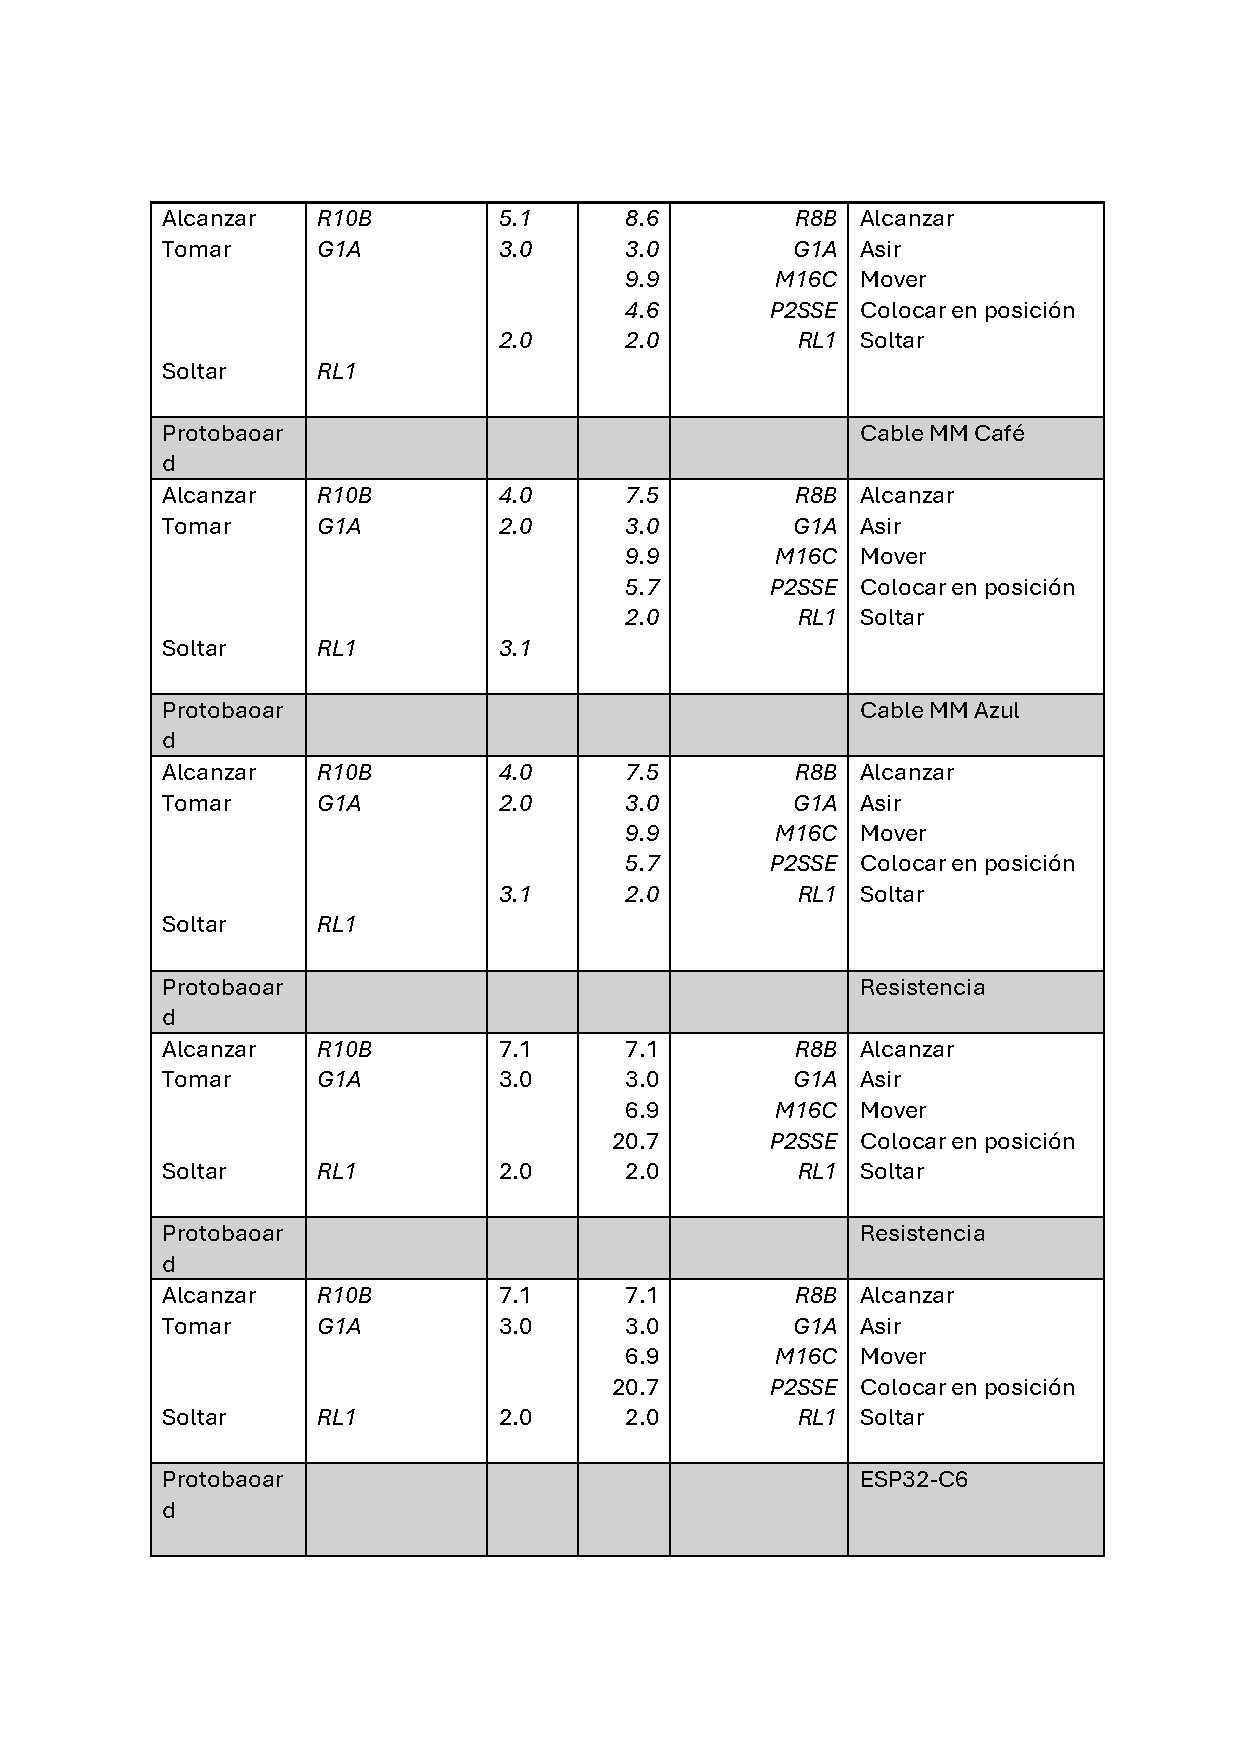
\includegraphics[trim = {40mm 60mm 20mm 21mm},clip,scale=0.35]{9/Img/tablaMtmDos.pdf}
        \label{fig:MtmDos}
    \end{figure}
    %
    \begin{figure}[H]
        \centering
        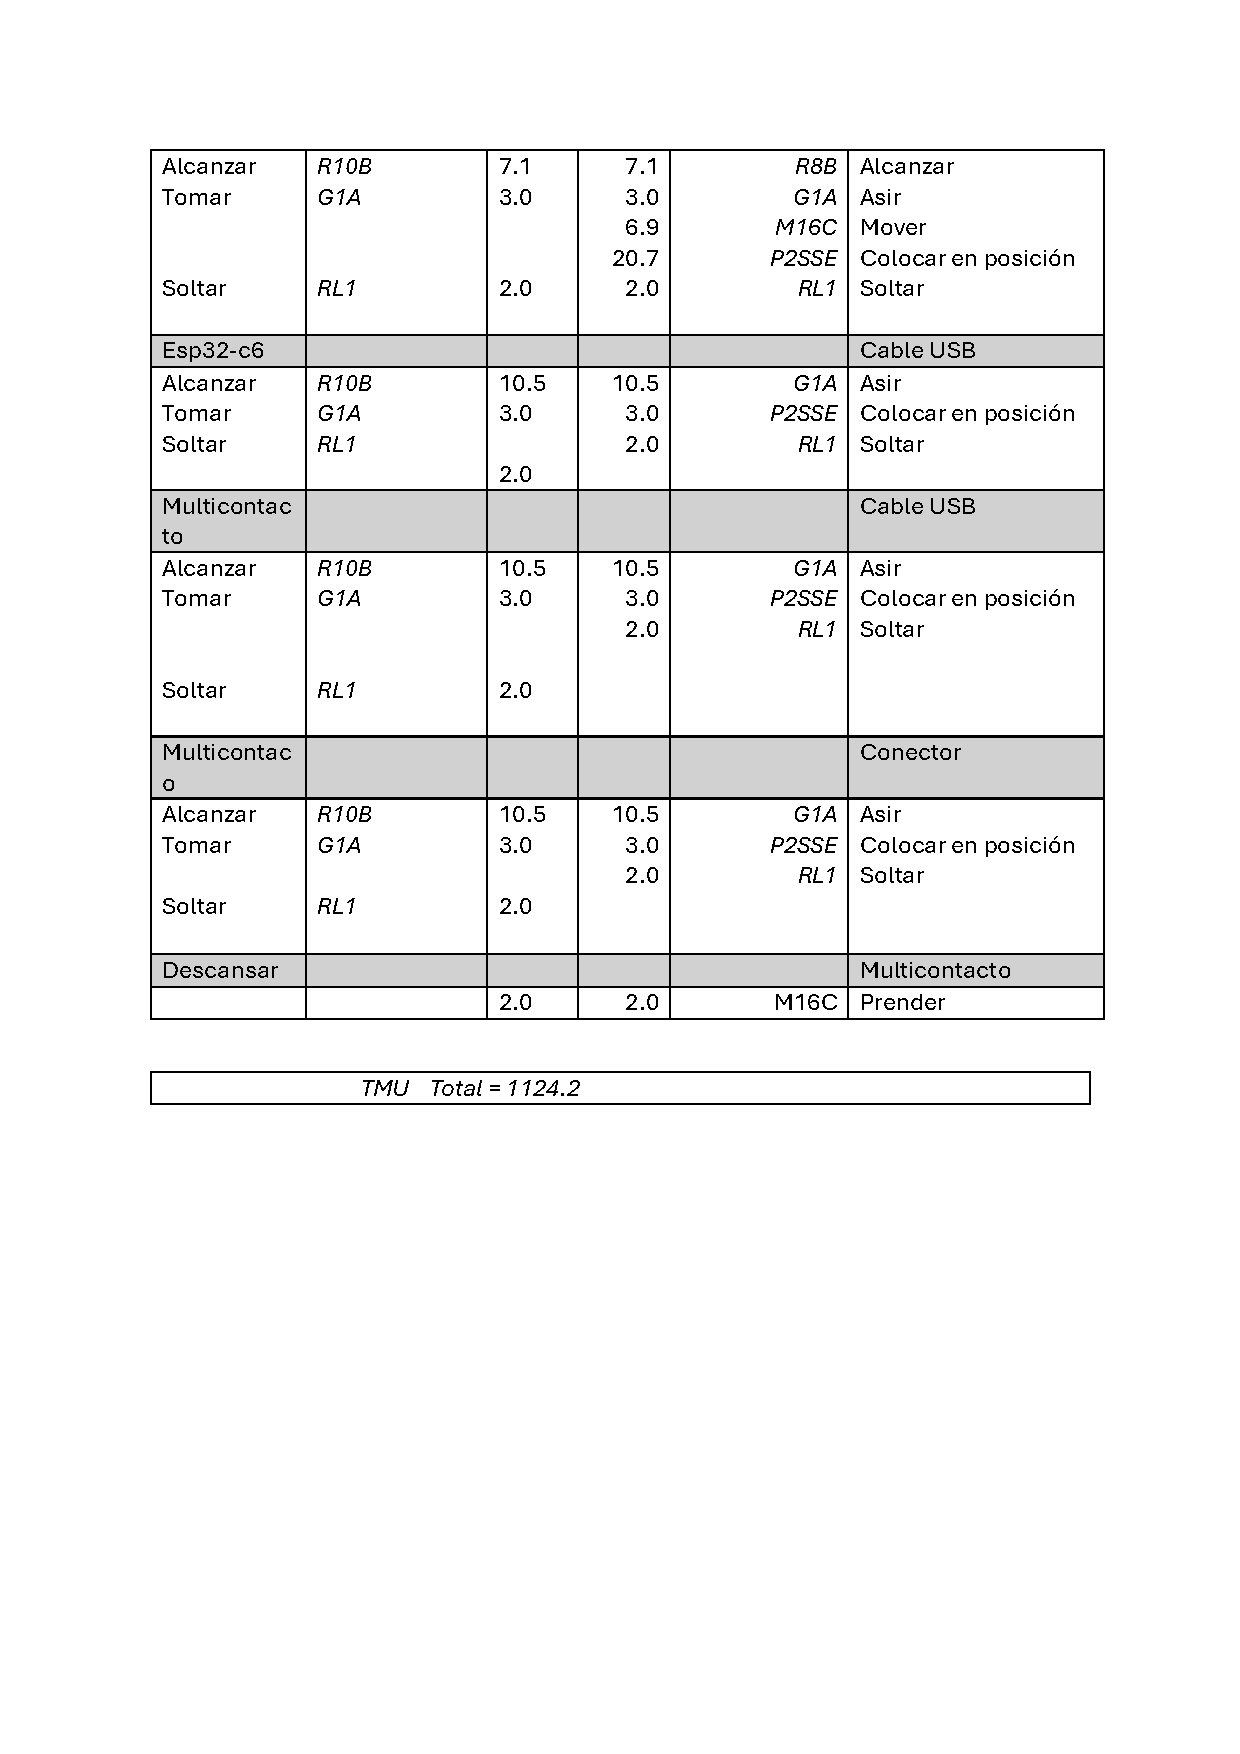
\includegraphics[trim = {40mm 60mm 20mm 21mm},clip,scale=0.35]{9/Img/tablaMtmTres.pdf}
        \label{fig:MtmTres}
    \end{figure}
    \subsubsection{Desarrollo del muestreo del trabajo}
    %
    \begin{figure}[H]
        \centering
        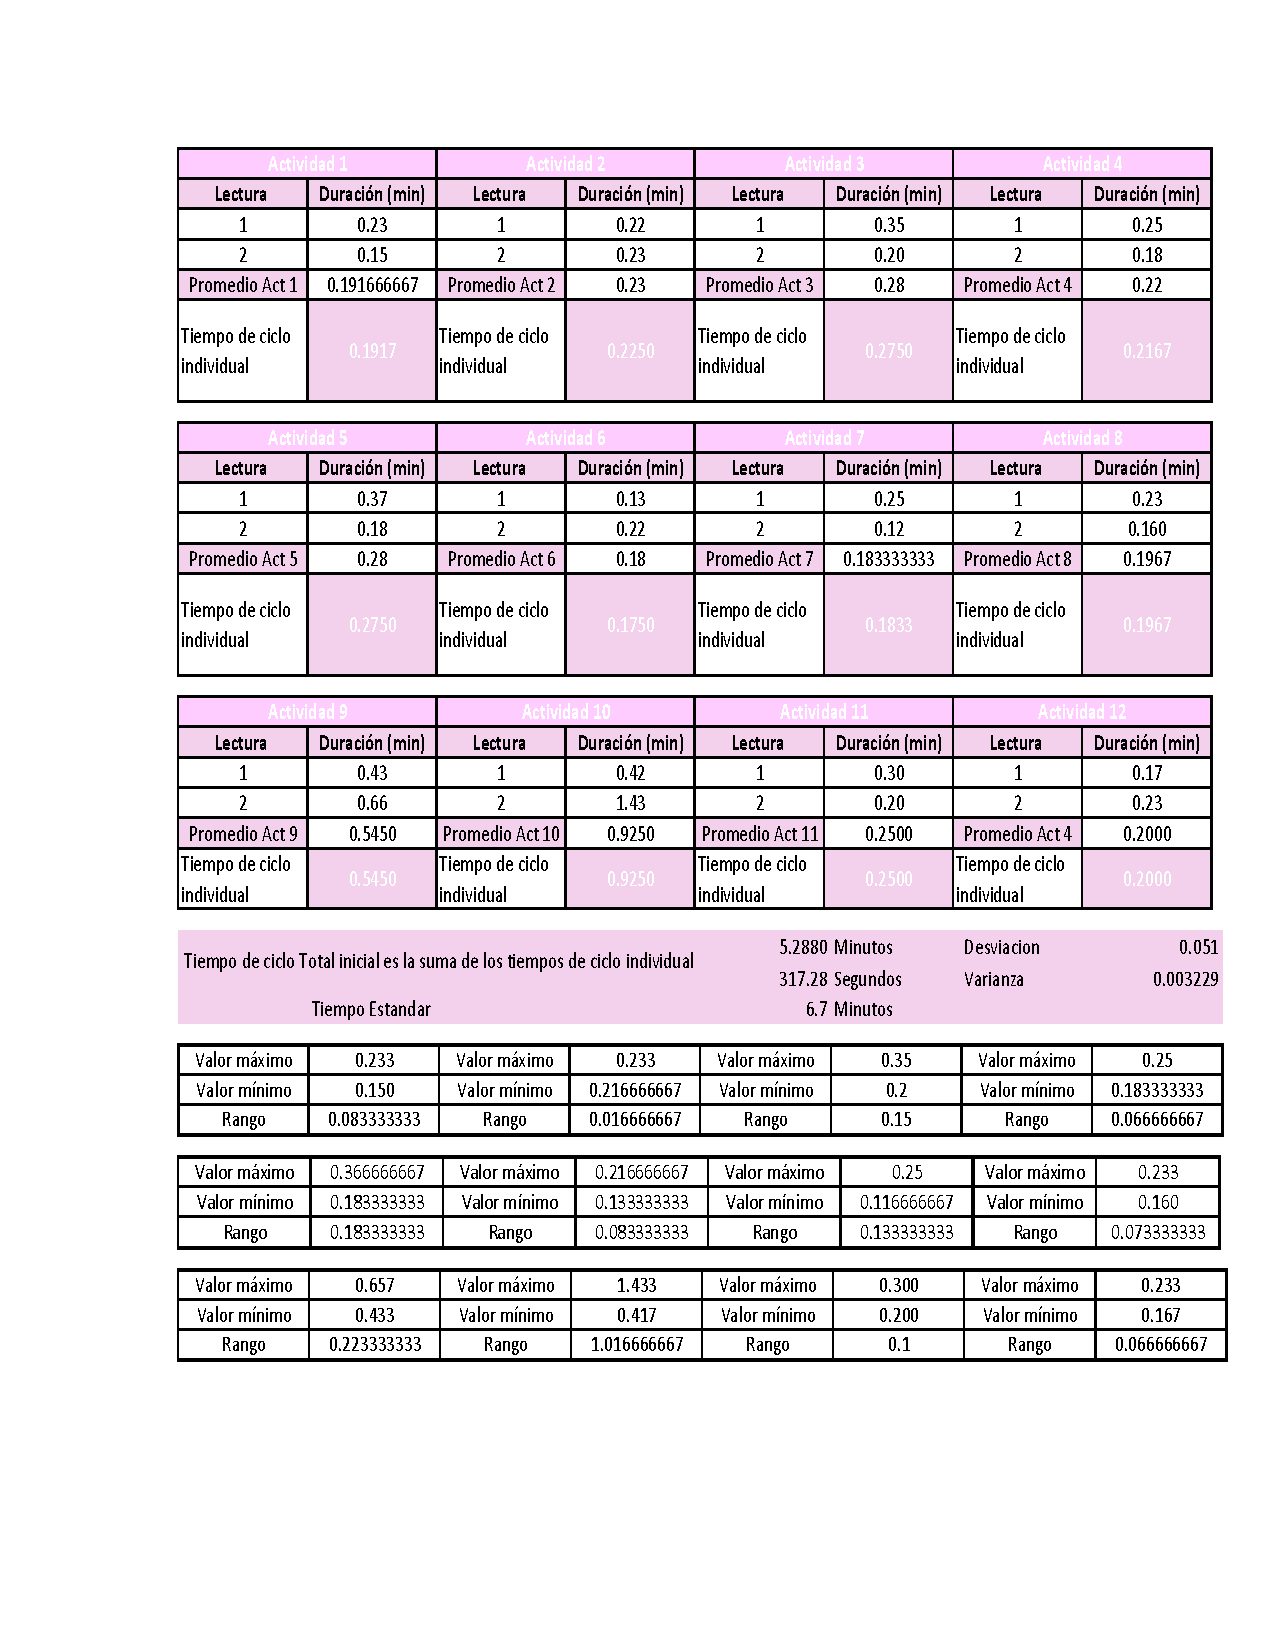
\includegraphics[scale=0.3]{9/Img/tiempoCiclo.pdf}
        \caption{Tiempo Ciclo}
        \label{fig:tiempo Ciclo}
    \end{figure}
    %
    \begin{figure}[H]
        \centering
        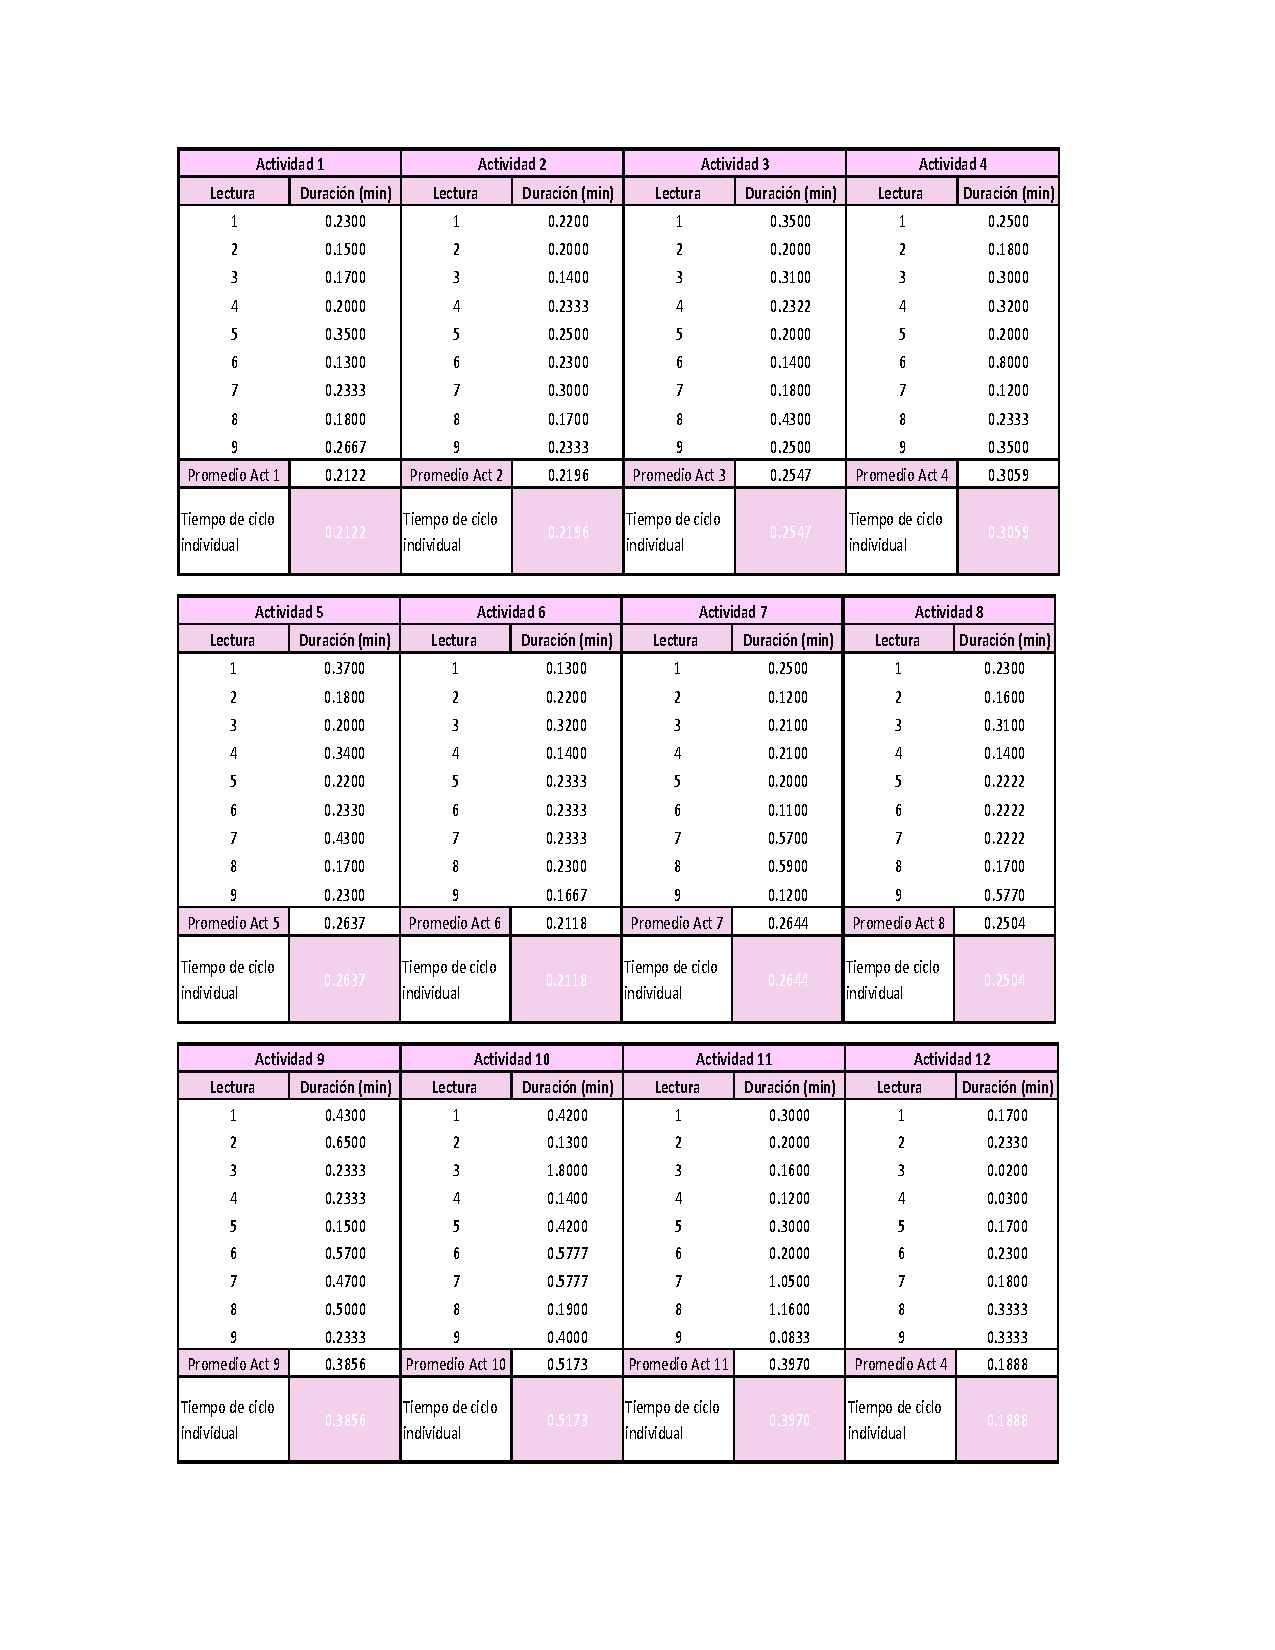
\includegraphics[scale=0.3]{9/Img/muestreo.pdf}
        \caption{Muestreo}
        \label{fig:muestreo}
    \end{figure}
    %
    \begin{figure}[H]
        \centering
        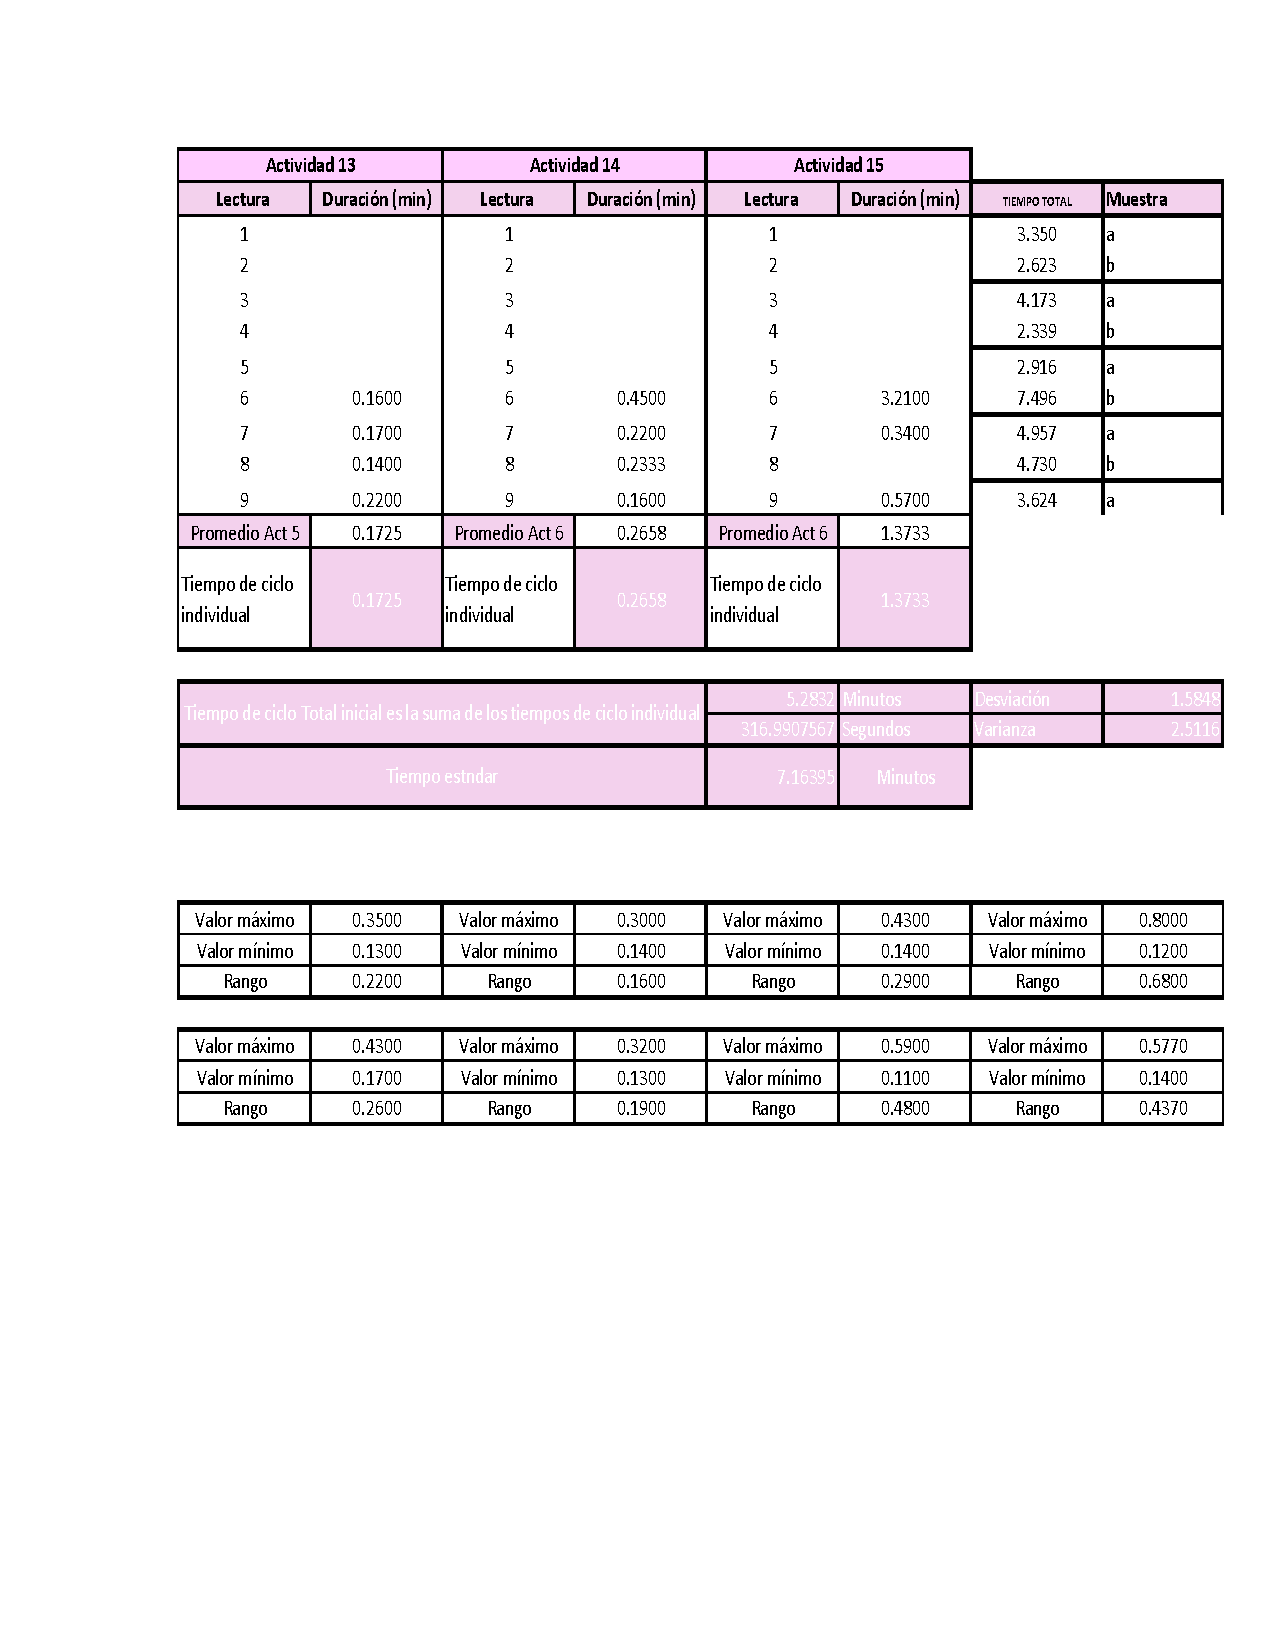
\includegraphics[scale=0.3]{9/Img/muestreoUno.pdf}
        \caption{Muestreo}
        \label{fig:muestreo}
    \end{figure}
    %
    \subsubsection{Corrección por balanceo de procesos}
    %
    Para garantizar un buen manejo de tareas sera fundamental el uso del balanceo de lineas. Se lograra un flujo de Producción constante para optimizar los costos al igual que mejorar la calidad.
    En resumen, el balanceo de líneas es una práctica fundamental en la gestión de la producción que busca mejorar la productividad, reducir los tiempos de espera y aumentar la calidad de los productos fabricados.
    %
    \subsubsection{Datos estándar continuos y discretos}
    
    %
    \subsection{Diseño de la forma más económica de realizar el trabajo}
    
    %
    \subsection{Normalización de los métodos, materiales, herramientas e instalaciones}
    %
    \subsection{Determinación del tiempo estándar para que una persona competente realice el trabajo con marcha normal}
    %
    
    \section{Conclusiones}
    %
    Al desarrollar el proyecto integrador logramos desarrollar nuevos Métodos, procesos y herramientas empleadas en la materia Estudio Del Trabajo II, así mismo se logro incrementar varios puntos importantes como el plan de emergencia, la Localización,  identificación de apoyos externos en caso de necesidad eh Identificación de riesgos.   
    %
    Al finalizar las 2 muestras las cuales se muestra en la siguiente tabla\ref{fig:tiempo Ciclo} podemos obtener un tiempo ciclo de 5.28 minutos Con el muestreo realizado logramos obtener distintas muestras las cuales podemos ver en las siguientes\ref{fig:muestreo} estas nos sirvieron de ayuda para determinar nuestro tiempo estándar el cual fue de 7.16 minutos posteriormente se realizo un balance de líneas y poder reducir nuestros tiempos con ayuda de los therblings obteniendo una producción balanceada y con un costo de producción bajo con esto cumplimos la etapa del estudio de movimientos y tiempos. Se logro establecer un tiempo estándar de 6.7 minutos para el ensamble aplicando los STP y el uso de probabilidades. 
    %
    Comparando los resultados mostrados por los diferentes métodos debo de concluir por aquel que sea mas conveniente, el mas conveniente es el tiempo estándar de 6.7 minutos, ya que tiene un tiempo adecuado para el proceso del ensamble a diferencia del otro método realizado. 
    %
    Podemos concluir que este proyecto nos dejo varias herramientas de apoyo como fueron Overleaf, Github, las cuales  serán de gran utilidad en todo nuestro proceso universitario.
    Fue fundamental la dedicación, el compromiso y la colaboración de todos los miembros para alcanzar el éxito en la ejecución del trabajo.
    %
    
    \section{Agradecimientos}
    
    Es importante darles su debido reconocimiento a los laboratorios, instituciones, organizaciones, entre otros que han sido participes para la culminación de este trabajo. También es importante mencionar, fondos, proyectos, becas, entre otros que se le han otorgado al o los autores para realizar el trabajo de investigación. Ejemplo: “Los autores agradecen al Concejo Nacional de Ciencia y Tecnología por los recursos otorgados…”
    
    \section*{Referencias}
    
    
    
    
    
    % Otros ejemplos \cite{LAAngeles2021}, \cite{LAAngelesConni}. 
    %Véase el link \cite{prueba}.
    
    
    
    % Ejemplo
    %  @Article{article,
    % 	author = "Author1 LastName1 and Author2 LastName2 and Author3 LastName3",
    % 	title = "Article Title",
    % 	volume = "30",
    % 	number = "30",
    % 	pages = "10127-10134",
    % 	year = "2013",
    % 	doi = "10.3389/fnins.2013.12345",
    % 	URL = "http://www.frontiersin.org/Journal/10.3389/fnins.2013.12345/abstract",
    % 	journal = "Frontiers in Neuroscience"
    % }
    
    % @book{book,
    %   author    = {Author Name}, 
    %   title     = {The title of the work},
    %   publisher = {The name of the publisher},
    %   address   = {The city},
    %   year      = 1993,
    % }
    
    % @incollection{chapter,
    %   author       = {Bauthor Surname}, 
    %   title        = {The title of the work},
    %   editor       = {Editor Name},
    %   booktitle    = {The title of the book},
    %   publisher    = {The name of the publisher},
    %   address      = {The city},
    %   year         = 2002,
    %   pages        = {201-213},
    % }
    
    % @InProceedings{conference,
    %   author = {Cauthor Name and Dauthor Surname and Fauthor LastName},
    %   title = {The title of the work},
    %   booktitle = {The title of the conference proceedings},
    %   year = 1996,
    %   publisher = {The name of the publisher},
    %   editor = {Editor Name1 and Editor Name2},
    %   pages = {41-50},
    % }
    
    % @book{cho,
    %   author       = {Gauthor Name1}, 
    %   title        = {The title of the work},
    %   publisher = {Country code and patent number},
    %   address      = {Patent Country},
    %   year = 2013
    % }
    
    % @book{patent,
    %   author    = {Hauthor Surname1}, 
    %   title     = {The title of the work},
    %   publisher = {Patent number},
    %   address   = {Patent country},
    %   year      = 2010,
    % }
    
    % % please use misc for datasets
    % @misc{dataset, 
    % 	author = "Author1 LastName1 and Author2 LastName2 and Author3 LastName3",
    % 	title = "Data Title",
    % 	year = "2011",
    % 	doi = "10.000/55555",
    % 	URL = "http://www.frontiersin.org/",
    % }
    
    \bibliographystyle{ieeetr}
    \bibliography{9/referencias}
    % 
    % 
    %%%%%%%%%%%%%%%%%%%%%%%%%%%%%%%%%%
    \appendix
    %%%%%%c%%%%%%%%%%%%%%%%%%%%%%%%%%%%
    % 
    
    %%%%%%%%%%%%%%%%%%%%%%%%%%%%%%%%%%%%%%%%